%% 
%% Copyright 2019-2020 Elsevier Ltd
%% 
%% This file is part of the 'CAS Bundle'.
%% --------------------------------------
%% 
%% It may be distributed under the conditions of the LaTeX Project Public
%% License, either version 1.2 of this license or (at your option) any
%% later version.  The latest version of this license is in
%%    http://www.latex-project.org/lppl.txt
%% and version 1.2 or later is part of all distributions of LaTeX
%% version 1999/12/01 or later.
%% 
%% The list of all files belonging to the 'CAS Bundle' is
%% given in the file `manifest.txt'.
%% 
%% Template article for cas-sc documentclass for 
%% double column output.

%\documentclass[a4paper,fleqn,longmktitle]{cas-sc}
\documentclass[a4paper,fleqn]{cas-sc}

% \usepackage[numbers]{natbib}
\usepackage[authoryear]{natbib}
% \usepackage[authoryear,longnamesfirst]{natbib}

%%%Author definitions
\def\tsc#1{\csdef{#1}{\textsc{\lowercase{#1}}\xspace}}
\tsc{WGM}
\tsc{QE}
\tsc{EP}
\tsc{PMS}
\tsc{BEC}
\tsc{DE}
%%%

% Uncomment and use as if needed
%\newtheorem{theorem}{Theorem}
%\newtheorem{lemma}[theorem]{Lemma}
%\newdefinition{rmk}{Remark}
%\newproof{pf}{Proof}
%\newproof{pot}{Proof of Theorem \ref{thm}}

\begin{document}
\let\WriteBookmarks\relax
\def\floatpagepagefraction{1}
\def\textpagefraction{.001}


% Short author
\shortauthors{Hao Wang et~al.}
\shorttitle{}

% Main title of the paper
\title [mode = title]{Cooperative Adaptive Cruise Platoon Controller Design Considering Head-to-tail String Stability and Control Switching}
% Title footnote mark
% eg: \tnotemark[1]
% \tnotemark[1,2]

% Title footnote 1.
% eg: \tnotetext[1]{Title footnote text}
% \tnotetext[<tnote number>]{<tnote text>} 
% \tnotetext[1]{This document is the results of the research
%    project funded by the National Science Foundation.}

% \tnotetext[2]{The second title footnote which is a longer text matter
%    to fill through the whole text width and overflow into
%    another line in the footnotes area of the first page.}


% First author
%
% Options: Use if required
% eg: \author[1,3]{Author Name}[type=editor,
%       style=chinese,
%       auid=000,
%       bioid=1,
%       prefix=Sir,
%       orcid=0000-0000-0000-0000,
%       facebook=<facebook id>,
%       twitter=<twitter id>,
%       linkedin=<linkedin id>,
%       gplus=<gplus id>]
\author[1,2,3]{Hao Wang}[style=chinese]
% Corresponding author indication
\cormark[1]

% % Footnote of the first author
% \fnmark[1]

% Email id of the first author
\ead{haowang@seu.edu.cn}

% % URL of the first author
% \ead[url]{www.cvr.cc, cvr@sayahna.org}

%  Credit authorship
\credit{Conceptualization of this study, Formal analysis,Funding acquisition,Supervision,Writing - review \& editing}

% Address/affiliation
\affiliation[1]{organization={Jiangsu Key Laboratory of Urban ITS, Southeast University},
  addressline={2 Si Pai Lou},
  city={Nanjing},
  % citysep={}, % Uncomment if no comma needed between city and postcode
  postcode={210096},
  % state={},
  country={P.R. China}}

\affiliation[2]{organization={Jiangsu Province Collaborative Innovation Center of Modern Urban Traffic Technologies},
  addressline={2 Si Pai Lou},
  city={Nanjing},
  % citysep={}, % Uncomment if no comma needed between city and postcode
  postcode={210096},
  % state={},
  country={P.R. China}}
\affiliation[3]{organization={School of Transportation, Southeast University},
  addressline={2 Si Pai Lou},
  city={Nanjing},
  % citysep={}, % Uncomment if no comma needed between city and postcode
  postcode={210096},
  % state={},
  country={P.R. China}}
% Second author
\author[1,2,3]{Tiancheng Ruan}[style=chinese]
\ead{ruantiancheng@seu.edu.cn}
\credit{ Methodology,Writing - Original draft preparation,Resources, Software}

% Third author
\author[1,2,3]{Linjie Zhou}[style=chinese]
% \fnmark[2]
\ead{220193107@seu.edu.cn}
% \ead[URL]{www.sayahna.org}
\credit{Data curation,Investigation}


\author[1,2,3]{YuXuan Hou}[style=chinese]
\ead{NOTEVENWRONG@outlook.com}
\credit{Formal analysis,Writing - Original draft preparation}



% Fourth author
\author%
[4]
{Rui Jiang}
\cormark[1]
% \fnmark[1,3]
\ead{jiangrui@bjtu.edu.cn}
\credit{ Data curation,Writing - review \& editing}

\affiliation[4]{organization={Key Laboratory of Transport Industry of Big Data Application Technologies for Comprehensive Transport, Ministry of Transport, Beijing Jiaotong University},
  city={Beijing},
  % citysep={}, % Uncomment if no comma needed between city and postcode
  postcode={100044},
  % state={},
  country={P.R. China}}

% \affiliation[4]{organization={MOE Key Laboratory for UrbanTransportation Complex Systems Theory and Technology, Beijing Jiaotong University},
%     city={Beijing},
%     % citysep={}, % Uncomment if no comma needed between city and postcode
%     postcode={100044}, 
%     % state={},
%     country={P.R. China}}
% \affiliation[5]{organizati on={State Key Laboratory of Fire Science and School of Engineering Science, University of Science and Technology of China},
%     city={Hefei},
%     % citysep={}, % Uncomment if no comma needed between city and postcode
%     postcode={230026}, 
%     % state={},
%     country={P.R. China}}



% Corresponding author text
\cortext[cor1]{Corresponding author}

% Footnote text
% \fntext[fn1]{This is the first author footnote. but is common to third
%   author as well.}
% \fntext[fn2]{Another author footnote, this is a very long footnote and
%   it should be a really long footnote. But this footnote is not yet
%   sufficiently long enough to make two lines of footnote text.}

% For a title note without a number/mark
% \nonumnote{This note has no numbers. In this work we demonstrate $a_b$
%   the formation Y\_1 of a new type of polariton on the interface
%   between a cuprous oxide slab and a polystyrene micro-sphere placed
%   on the slab.
%   }

% Here goes the abstract
\begin{abstract}
  % With the development of Cooperative adaptive cruise control (CACC) technology,  CACC Market Penetration Rate (MPR) is expected to increase rapidly in the near future, which will result in more CACC platoons. Controller design seeking strict string stability is unable to take full advantage of CACC platoons which can maintain head-to-tail stability with a smaller desired time gap. This paper first proposed a novel CACC controller design mode— Cooperative Adaptive Cruise Platoon Control (CACPC)—that takes the CACC platoon as the control object to further use CACC technology. Secondly, an online-switching method, Youla-Kučera (YK) parameterization, was adopted to ensure stability while switching the two control modes under different platoon sizes. Finally, numerical analyses and simulations were conducted to explore the effectiveness of CACPC on dynamic performance and traffic capacity. It is found that YK parameterization can significantly suppress the perturbation caused by the switching of control mode and maintain stability during the switching. Besides, CACPC can gain traffic capacity, which is 1.52 times the case without CACPC and 3.02 times the case of pure MV when CACC MPR is 100\%.
  With the development of Cooperative Adaptive Cruise Control (CACC) technology, CACC Market Penetration Rate (MPR) is expected to increase rapidly in the near future, which will result in more CACC platoons. Controller design seeking strict string stability is unable to take full advantage of CACC platoons which can maintain head-to-tail stability with a smaller desired time gap. This paper first proposed a novel CACC controller design mode— Cooperative Adaptive Cruise Platoon Control (CACPC)—that takes the CACC platoon as the control object to further use CACC technology. Secondly, an control switching method, Youla-Kučera (YK) parameterization, was adopted to ensure stability while switching the two control modes under different platoon sizes. Finally, numerical analyses and simulations were conducted to explore the effectiveness of CACPC on dynamic performance. It is found that YK parameterization can significantly suppress the perturbation caused by the switching of control mode and maintain stability during the switching.
\end{abstract}

% Use if graphical abstract is present
% \begin{graphicalabstract}
% 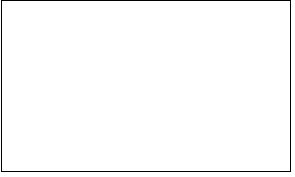
\includegraphics{figs/grabs.pdf}
% \end{graphicalabstract}

% Research highlights
\begin{highlights}
  \item Adopted head-to-tail string stability analyses for controller design.
  \item Proposed a CACC platoon control which is adaptable for any platoon size.
  \item Applied YK parameterization to ensure stable interpolation between controllers.
  \item Parameters of the lower control level of vehicle is calibrated by field tests.
  \item Explored a gain-scheduling scheme of CACC platoon to make it stable and effective.
\end{highlights}

% Keywords
% Each keyword is seperated by \sep
\begin{keywords}
  Cooperative adaptive cruise control \sep Platoon control \sep Head-to-tail string stability \sep Switching control
\end{keywords}


\maketitle

\section{Introduction}
\label{Section 1}
To maintain safety, mobility, and environmental sustainability as transportation systems develop rapidly, Connected Autonomous Vehicle (CAV) technology has burgeoned and attracted considerable attention in the past decade. The connectivity and automation of the vehicle have been significantly improved. Vehicle-to-Infrastructure (V2I) communication technology guarantees partial or full automation with the help of in-vehicle sensors, and Vehicle-to-Vehicle (V2V) communication technology enables communication and cooperation between vehicles \citep{wang2019survey,ploeg2011design,zhou2021impact}.

The most typical application of V2V communication is Cooperative Adaptive Cruise Control (CACC). A vehicle controlled by this type of system automatically follows the preceding vehicles. Simulation results and field experiments reveal that, compared with traditional vehicles, cooperatively controlled CAVs can maintain a shorter time headway between vehicles. Therefore, consecutively connected vehicles can form a platoon-based driving mode through Cellular vehicle-to-everything (C-V2X) communication to improve traffic efficiency \citep{gong2018cooperative,wang2020cooperative}.

According to the literature \citep{qin2018stability,ruan2021stability}, standard car-following models should guarantee local stability, which means perturbations will gradually disappear over time. Furthermore, most CACC controllers are designed for maintaining the strict string stability of CACC platoon \citep{wang2018infrastructure,sun2018stability,ploeg2013lp} which will inevitably lead to much redundancy hence the need for optimization.

Moreover, it will take a long time for CACC MPR to grow due to the immaturity of CACC technology, as the CACC MPR is projected to be only 24.8\% in 2045, according to the latest research \citep{Bansal2017}. Moreover, since a small amount of CACCs cannot guarantee that communication functions properly, most CACCs will degrade into Adaptive Cruise Controls (ACCs) \citep{ruan2021stability,qin2018stability}. Therefore, the performance of short CACC platoon is still worth studying.

In order to the leverage the benefit of CACCs, this paper proposed a new decentralized control mode named Cooperative Adaptive Cruise Platoon Control (CACPC) that has taken the CACC platoon as the control object instead of a single vehicle. Firstly, we explored the combination of margin stable desired time gap under different platoon sizes using string stability analyses. Secondly, Youla-Kučera (YK) parameterization was adopted to guarantee smoothness and stability in the switching of control mode. Thirdly, a tuning function was proposed to ensure the application under different platoon sizes. Finally, the effectiveness of CACPC on dynamic performance was explored.

The rest of this paper is organized as follows. Section~\ref{Section 2} introduces the CACC system setup, control objectives, and control structure studied in this paper. Section~\ref{Section 3} proposes the primary methodology includes string stability analyses and YK parameterization. The theoretical results are presented in Section~\ref{Section 4}. Section~\ref{Section 5} validates the theoretical results and explores the impact of CACPC. The conclusion is summarized in Section~\ref{Section 6}.

\section{Problem Formulation}
\label{Section 2}
This section mainly introduces the background knowledge of the problems studied in this paper from three perspectives: CACC system setup, control objectives, and control structure.

\subsection{CACC System Setup}
\label{Section 2.1}

\begin{figure}
  \centering
  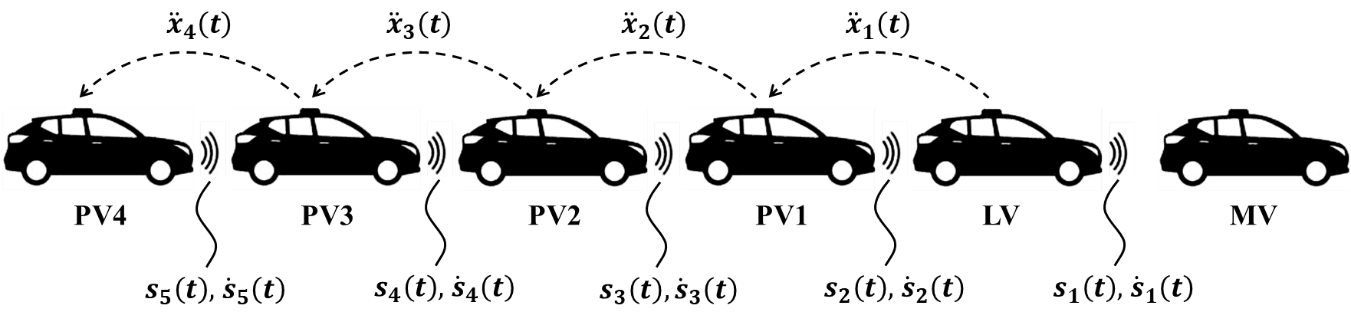
\includegraphics[width=14cm]{figs/fig1.png}
  \caption{~Schematic of CACC platoon.}
  \label{fig1}
\end{figure}

Fig.~\ref{fig1} shows a schematic of the CACC platoon, where $s_i (t)$,$\dot{s}_{i} (t)$ indicate the relative gap and relative velocity that CACC obtained through the onboard sensor, and $\ddot{x}_{i-1} (t)$ is the acceleration of the predecessor vehicle obtained through V2V communication.

The CACC design is based on a standard ACC system equipped with a communication module. A CACC platoon can be divided into an Leader Vehicle (LV) and S-1 Platoon vehicles (PV)s based on the communication ability of the predecessor vehicle, where S denotes the maximum size of a CACC platoon. Notice that we think the CACC platoon can not be infinitely long due to the limitation of unreliable communication environment and we assume the maximum platoon size is the platoon size which can keep communication function well. The LVs degrades to ACCs functionally because the predecessor vehicle is ACC or MV and cannot communicate, while the communication module of PVs is functioning \citep{dey2015review,navas2019mixing}.

Considering the feasibility of implementation, the controller used in this paper is a decentralized controller instead of a centralized one. The specific information flow topology (IFT) is predecessor following (PF) which means CACCs only communicate with the nearest predecessor to gain further information in advance. As for spacing policy, Constant Time Gap (CTG), including a constant part and a velocity-dependent part, is applied due to its widespread use.

\subsection{String stability}
\label{Section 2.2}

We have considered the nuances in different definitions of string stability in the literature. In this paper, the "head-to-tail" string stability is adopted. Namely, the perturbation will not be amplified during upstream propagation \citep{qin2021analytical,montanino2021homogeneous,jin2014dynamics,zhou2020stabilizing,wang2018infrastructure}, i.e., from vehicle LV to vehicle PV4 (see Fig.~\ref{fig1}). As for specific spacing policy, the error $e_i (t)$ between the desired and actual inter-vehicle gap is frequently considered in CTG to prevent collisions.

In this paper, the head-to-tail string stability of the CACC platoon is studied as a whole instead of analyzing each CACC in the platoon. To facilitate the analysis and focus on the amplification of perturbation, a frequency-domain approach is adopted to obtain a necessary and sufficient condition for the head-to-tail string stability of the CACC platoon, which will provide support for designing CACPC.

\subsection{Control Structure}
\label{Section 2.3}
The CACC design is based on a standard ACC system and applies the most commonly used CTG policy. In this subsection, the control structures of the ACC and CACC system are discussed respectively in order to study the subsequent design of CACPC.

It is assumed that each CACC is equipped with i) an on-board radar responsible for collision detection via measuring the gap distance between any two consecutive vehicles, ii) a built-in GPS sensor for measuring the vehicular longitudinal position information, iii) a wireless on-board unit for communicating information of interest with its proximal vehicles via the C-V2X communication, iv) an upper-level controller for calculating the desired longitudinal acceleration based on the parameters obtained, and v) a lower-level controller for determining the throttle and brake actuator inputs so as to track the desired acceleration. Such an assumption is reasonable as the sensing, communication, and actuation units requested above are available in modern CAVs, and thus do not require specific changes in the existing vehicle configuration. Note that the on-board radar only functions when the CACC degrade to the ACC if communication is unavailable or malfunctioning since more accurate information can be obtained faster via communication.

Moreover, we remark that this paper only focus on the homogeneous CACCs where CACCs have same control structure and controller parameters.


\subsubsection{ACC Control Structure}
\label{Section 2.3.1}
The primary control object of the ACC system is to maintain the desired gap from the preceding vehicle $s_{d, i}(t)=r_{i}+L_{i}+h_{i} \dot{x}_{i}(t)$, including a velocity-dependent part and a constant part, where $L_i$ represents the vehicle length, $r_i$ is the standstill distance and $h_i$ is the desired time gap of vehicle i. Using the onboard sensor, the relative gap $s_{i}(t)=x_{i-1}(t)-x_{i}(t)$ and relative velocity $\dot{s}_{i} (t)$ are measured. In a standard ACC system, the feedback controller controls the error $e_{i}(t)=s_{i}(t)-s_{d, i}(t)$ between the desire gap and relative gap.

The ACC control structure is schematically depicted in Fig.~\ref{fig2} (a).

\begin{figure}
  \centering
  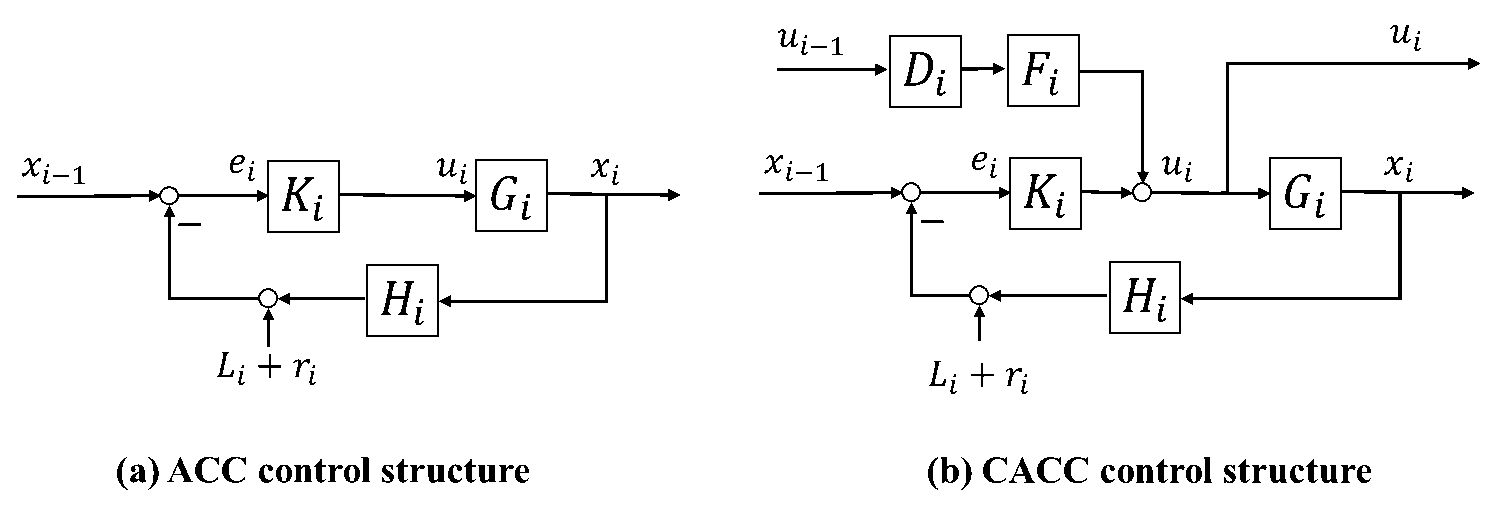
\includegraphics[width=14cm]{figs/fig2.png}
  \caption{~Control structure of ACC and CACC: (a) ACC; (b) CACC.}
  \label{fig2}
\end{figure}

As shown in Fig.~\ref{fig2} (a), the ACC control structure is represented as a system construction drawing with vehicle position as input and output. The model $K_i (s)$ is the ACC feedback gain, which can be given as:
\begin{equation}
  K_{i}(s)=k_{p}+k_{d} s,
\end{equation}
where $k_p$ is error gain and $k_d$ is error speed gain, the specific parameter setting is based on previous research \citep{milanes2014modeling,milanes2013cooperative}.

The model $G_i (s)$ represents a lower level controller longitudinal vehicle dynamics, where the input $u_i (t)$ of $G_i (s)$ is the desired acceleration derived from $K_i (s)$ and the output $x_i (t)$ is the output position based on the control loop to track desired acceleration through actuation of the throttle and brake system. The linear transfer function of $G_i (s)$ can be represented by \citep{ploeg2013lp}:
\begin{equation}
  G_{i}(s)=\frac{k_{G}}{s^{2}\left(\tau_{i} s+1\right)} e^{-\phi_{i} s},
\end{equation}
where $\tau_{i}^{-1}=\omega_{b w, l, i}$ is the closed-loop bandwidth, $k_G$ is the model gain and $\phi_{i}$ is the time delay of vehicle actuator and communication, the specific parameter setting is shown in Table.~\ref{table1}.

Model $H_i (s)$ is the ACC feedback gain, which can be given as:
\begin{equation}
  H_{i}(s)=1+h_{i} s,
\end{equation}
where $h_i$ is the desired time gap of vehicle i.

The closed-loop transfer function of ACC system in the frequency domain is as follows:
\begin{equation}
  \mathcal{J}_{i, A C C}(s)=\frac{X_{i}(s)}{X_{i-1}(s)}=\frac{G_{i}(s) K_{i}(s)}{1+H_{i}(s) G_{i}(s) K_{i}(s)},
\end{equation}
where $X_i (s)$ is the Laplace transform of $x_i (t)$.

\subsubsection{CACC Control Structure}
\label{Section 2.3.2}

As discussed above, the CACC controller is equipped with a communication module that extended the standard ACC feedback controller. The specific control structure is schematically depicted in Fig.~\ref{fig2} (b).

For simplicity, the definitions of model $H_i(s)$,$G_i(s)$,$K_i(s)$ in system construction drawing are omitted because they are the same as those in Section~\ref{Section 2.3.1}. The acceleration $\ddot{x}_{i-1}(t)$ of predecessor vehicle obtained through V2V communication is used as a feedforward control signal through the feedforward filter $F_i(s)$ and the communication delay model $D_i(s)$.

The model $D_i(s)$ is directly related to the constant communication delay $\theta_i$, which can be expressed as:
\begin{equation}
  D_{i}(s)=e^{-\theta_{i} s},
\end{equation}
where $\theta_i$ represents the constant communication delay. The specific parameter setting is according to previous researches \citep{navas2016using,zhang2020control}.

The model $F_i(s)$ is the communication feedforward filter which can be given as:
\begin{equation}
  F_{i}(s)=\left(H_{i}(s) G_{i}(s)\right)^{-1}.
\end{equation}

The closed-loop transfer function of CACC system in the frequency domain is as follows:
\begin{equation}
  \mathcal{J}_{i, C A C C}(s)=\frac{X_{i}(s)}{X_{i-1}(s)}=\frac{\left(K_{i}(s)+D_{i}(s) F_{i}(s)\right) G_{i}(s)}{1+H_{i}(s) G_{i}(s) K_{i}(s)}.
\end{equation}

\subsubsection{CACPC structure}
\label{Section 2.3.3}

\begin{figure}
  \centering
  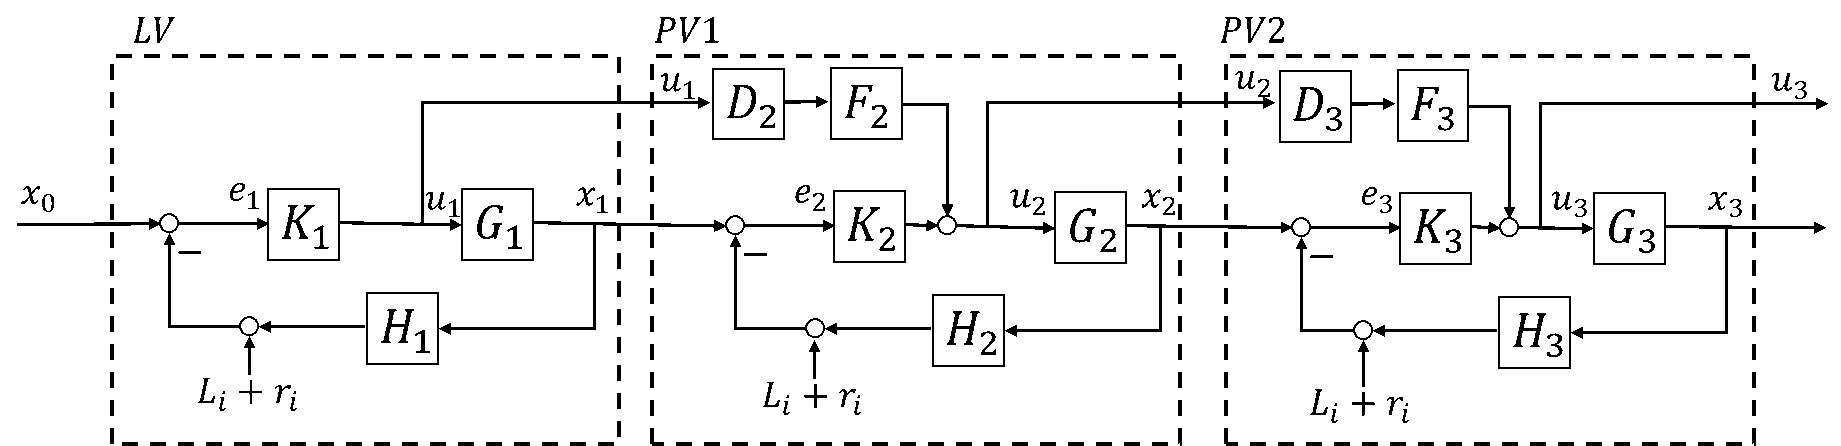
\includegraphics[width=14cm]{figs/fig3.png}
  \caption{~CACPC structure.}
  \label{fig3}
\end{figure}

As the control system for the controller design in this paper, the CACC platoon is designated as the primary control unit for string stability analyses. We can couple the control structure of ACC and CACC by merging the inner and outer signals, thus establishing the structure of CACPC. The specific structure of the CACPC is schematically depicted in Fig.~\ref{fig3}.

For simplicity, the definitions of model $H_i(s)$,$G_i(s)$, $K_i(s)$ and $D_i(s)$ in system construction drawing are omitted because they are the same as those in Section~\ref{Section 2.3.1} and ~\ref{Section 2.3.2}.

The closed-loop transfer function of CACPC system in the frequency domain is as follows:
\begin{equation}
  \mathcal{J}_{\text {platoon }}(s)=\frac{X_{n}(s)}{X_{0}(s)}=\frac{X_{n}(s)}{X_{n-1}(s)} \frac{X_{n-1}(s)}{X_{n-2}(s)} \ldots \frac{X_{1}(s)}{X_{0}(s)}=\mathcal{J}_{1, A C C}(s) \prod_{i=2}^{n} \mathcal{J}_{i, C A C C}(s),
  \label{Eq8}
\end{equation}
where n denotes the platoon size.

\section{Methodology}
\label{Section 3}
In this section, the primary methodology applied in this paper is introduced, including the transfer function method for string stability analyses and the YK parameterization for controller switching.

\subsection{String stability analyses}
\label{Section 3.1}

Laplace transform is a classic method to explore string stability in a direct and precise manner. Moreover, it has been adopted in several researches \citep{orosz2011delayed,montanino2021string,feng2019string}. Therefore, the head-to-tail string stability analyses of this paper are conducted based on the Laplace transform. The relationship of the perturbation propagating through CACC platoon in the frequency domain is:
\begin{equation}
  \mathcal{J}_{\text {platoon }}(s)=\frac{X_{n}(s)}{X_{0}(s)}.
\end{equation}

According to the definition of string stability, a sufficient and necessary conservative condition for string stability can be derived according to the $\mathcal{L}_{\infty}$ norm:
\begin{equation}
  \left\|x_{n}(t)\right\|_{\mathcal{L}_{\infty}} \leq \left\|x_{0}(t)\right\|_{\mathcal{L}_{\infty}}
  % \left\|\mathcal{J}_{\text {platoon }}(s)\right\|_{\mathcal{H}_{\infty}} \leq 1.
  \label{Eql_inf}
\end{equation}
where $x_{n}(t)$ and $x_{0}(t)$ are the inverse Laplace transformation of $X_{n}(s)$ and $X_{0}(s)$, respectively; $\|.\|_{\mathcal{L}_{\infty}}$ is the $\mathcal{L}_{\infty}$ norm, which deals with the deal with the peak of perturbations.

Moreover, according to the relationship $\|g\|_{1}=\sup _{x \in L_{\infty}} \frac{\|y\|_{\mathcal{L}_{\infty}}}{\|x\|_{\mathcal{L}_{\infty}}}$ Equation(\ref{Eql_inf}) can be replaced as:
\begin{equation}
  \|j\left(t\right)\|_{1}\leq 1
  \label{Eql_inf2}
\end{equation}
where $j\left(t\right)$ denotes the impulse response of $\mathcal{J}_{\text {platoon }}(s)$.

Furthermore, the Equation(\ref{Eql_inf2}) can be replaced by the following two conditions \citep{Swaroop1994}:
\begin{equation}
  \|\mathcal{J}_{\text {platoon }}(s)\|_{\infty} \leq 1 \& \quad j\left(t\right)>0
  \label{Eql_inf3}
\end{equation}

We remark that we adopt $\mathcal{L}_{\infty}$ norms of the string stability instead of $\mathcal{L}_{2}$ norms. Although $\mathcal{L}_{2}$ norms can provide clearer derivation, it only deals with the energy dissipation in the upstream direction and not the peak of perturbations \citep{Darbha2003}. In addition, the head-to-tail string stability, also named weakly single final string stability, is adopted in this paper for string stability analyses since it can deal with the relationship between peaks of perturbation before and after it spread over the platoon. So that the string stability indicates the perturbation is not amplified by the CACC platoon \citep{Studli2017}.
% Meanwhile, if $s=j\omega$, according to the definition of Laplace transform, we have:
% \begin{equation}
%   \left\|\mathcal{J}_{\text {platoon }}(j \omega)\right\|_{\mathcal{H}_{\infty}} \leq 1.
% \end{equation}

% Based on the transfer function of CACPC Equation(\ref{Eq8}), the following relation can be derived from linear system theory:
% \begin{equation}
%   \left\|\mathcal{J}_{\text {platoon }}(j \omega)\right\|_{\mathcal{H}_{\infty}}=\left\|\mathcal{J}_{1, A C C}(j \omega) \prod_{i=2}^{n} \mathcal{J}_{i, C A C C}(j \omega)\right\|_{\mathcal{H}_{\infty}}=\max _{x_{0} \neq 0} \frac{\left\|x_{n}(t)\right\|_{\mathcal{L}_{2}}}{\left\|x_{0}(t)\right\|_{\mathcal{L}_{2}}} \leq 1,
%   \label{Eq12}
% \end{equation}
% where $\mathcal{J}_{platoon}(j\omega)$ is the transfer function of CACC platoon evaluated on imaginary axis, $\|.\|_{\mathcal{H}_{\infty}}$ is the $\mathcal{H}_{\infty}$ norm, which means the supremum of $\mathcal{J}_{platoon}(j\omega)$ for all $\omega$, and$\|. \|_{\mathcal{L}_{2}}$ is the $\mathcal{L}_{2}$ norm.

% This condition can be interpreted as requiring energy dissipation in the upstream direction. This follows from the fact that, according to Equation(\ref{Eq12}), the $\mathcal{H}_{\infty}$ norm is induced by the $\mathcal{L}_{2}$ norms of input and output, which, in turn, are measures for energy. We remark that we adopt $\mathcal{L}_{2}$ norms of the string stability instead of $\mathcal{L}_{\infty}$ norms. Although

\subsection{Controller switching method: Youla-Kucera parametrization}
\label{Section 3.2}

Although the controllers are designed to maintain string stability of platoon under different platoon size, the switching of the controller will cause perturbations inevitably, which will cause safety hazards in the traffic flow. Therefore, a parameterization method for smooth switching between different controllers is needed to ensure the feasibility of the above CACC controller design.

Youla-Kucera (YK) parametrization is a method to stabilize the class of a given plant that contains all stablizing controllers \citep{dasgupta1996parametrization,navas2017youla}. One of the advantages of this method is that the performance transfer function is tuned with a special parameter, which means that the stability of unstable open-loop controllers can be maintained while switching between controllers.

\subsubsection{Fundamentals on YK parametrization}
\label{Section 3.2.1}

The basis of YK parametrization is described in detail below, which includes doubly coprime factorization and YK parameterization of all stabilizing controllers.

Basic notations are introduced below. $\mathbb{R} H_{\infty}$ is the real stable transfer function space; $G$ and $K_i$ maintain the same definitions as in Section~\ref{Section 3}.

For applying YK parametrization, internal dynamics of the vehicles G need to be presented as state-space representation:
\begin{equation}
  \begin{gathered}
    \dot{m}(t)=A m(t)+B u(t) \\
    x(t)=C m(t)+D u(t)
  \end{gathered}, G(s)=\left[\begin{array}{ll}
      A & B \\
      C & D
    \end{array}\right],
\end{equation}
where $t$ indicates time, $m(t)$ is the state vector, $\dot{m}(t)$ is the evolution of the state vector over time, $x(t)$ is the output vector, and $u(t)$ is the control vector. $A$, $B$, $C$, $D$ are the constant coefficients matrices of state-space matrices of $G$.

Any appropriate controller $K_i$ could stabilize this system, which is represented as:
\begin{equation}
  \begin{gathered}
    \dot{n}(t)=A_{i}^{c} n(t)+B_{i}^{c} e(t) \\
    u(t)=C_{i}^{c} n(t)+D_{i}^{c} e(t)
  \end{gathered}, K_{i}(s)=\left[\begin{array}{ll}
      A_{i}^{c} & B_{i}^{c} \\
      C_{i}^{c} & D_{i}^{c}
    \end{array}\right],
\end{equation}
where $n(t)$ is the state vector, and $A_i^c$,$B_i^c$,$C_i^c$ and $D_i^c$ are the constant coefficients matrices of state-space matrices of $K_i$. It should be noted that $K_0$ represents the initial controller and $K_1$ represents the controller after a complete switch, thanks to YK parametrization.

\subsubsection{Doubly coprime factorization}
\label{Section 3.2.2}

Factorization means the plant and controllers are represented as the products of two transfer functions. coprimeness refers to absence of common zeros in the right half-plane, and double coprimeness excludes unstable pole/zero cancellations, and refers to the idea of being right and left coprime.

The coprime factors of $G$ and $K_i$ can be expressed as:
\begin{equation}
  G=N M^{-1}=\tilde{M}^{-1} \tilde{N}, K_{i}=U_{i} V_{i}^{-1}=\tilde{V}_{i}^{-1} \tilde{U}_{i},
\end{equation}
where coprime factors $N, M, \tilde{M}, \tilde{N}, U_{i}, V_{i}, \tilde{U}_{i}, \tilde{V}_{i} \in \mathbb{R} H_{\infty}$ satisfy double Bezout's identity \citep{pommaret1998generalized}:
\begin{equation}
  \left[\begin{array}{cc}
      \tilde{V}_{i} & -\tilde{U}_{i} \\
      -\tilde{N}    & \tilde{M}
    \end{array}\right]\left[\begin{array}{cc}
      M & U_{i} \\
      N & V_{i}
    \end{array}\right]=\left[\begin{array}{cc}
      M & U_{i} \\
      N & V_{i}
    \end{array}\right]\left[\begin{array}{cc}
      \tilde{V}_{i} & -\tilde{U}_{i} \\
      -\tilde{N}    & \tilde{M}
    \end{array}\right]=\left[\begin{array}{cc}
      I & 0 \\
      0 & I
    \end{array}\right].
  \label{Eq16}
\end{equation}
Using the relationship of state-space representation and transfer function $G(s)=C(sI-A)^{-1} B$ and $K_i (s)=C_i^c (sI-A_i^c)^{-1} B_i^c+D_i^c$, coprime factors can be derived by:
\begin{equation}
  \left[\begin{array}{cc}
      M & U_{i} \\
      N & V_{i}
    \end{array}\right]=\left[\begin{array}{cc|cc}
      A+B F     & 0                             & -B & 0         \\
      0         & A_{i}^{c}+B_{i}^{c} F_{i}^{c} & 0  & B_{i}^{c} \\
      \hline -F & C_{i}^{c}+D_{i}^{c} F_{i}^{c} & I  & D_{i}^{c} \\
      -C        & F_{i}^{c}                     & 0  & I
    \end{array}\right],
  \label{Eq17}
\end{equation}
\begin{equation}
  \left[\begin{array}{cc}
      \tilde{V}_{i} & -\tilde{U}_{i} \\
      -\tilde{N}    & \tilde{M}
    \end{array}\right]=\left[\begin{array}{cc|cc}
      A+B  D_{i}^{c} C          & B  C_{i}^{c} & -B & B  D_{i}^{c} \\
      B_{i}^{c} C               & A_{i}^{c}    & 0  & B_{i}^{c}    \\
      \hline F_{i}- D_{i}^{c} C & -C_{i}^{c}   & I  & -D_{i}^{c}   \\
      C                         & -F_{i}^{c}   & 0  & I            \\
    \end{array}\right],
  \label{Eq18}
\end{equation}
where $F$ and $F_i^c$ should be chosen such that $A+BF$,$A_i^c+B_i^c F_i^c\in \mathbb{R} H_{\infty}$. Straight lines indicate the elements of the matrix that belong to each factor, respectively. The proof of the Equation (\ref{Eq17}-\ref{Eq18}) detailed in Appendix B.

During the process of controller switching, only the vehicle decision controller $K_i$ from $K_0$ switches to $K_1$ and internal dynamics of the vehicles G remain unchanged, which means $M$ and $N$ remain unchanged while $U_0$,$V_0$ are converted to $U_1$,$V_1$.

\subsubsection{YK parameterization of all stabilizing controllers}
\label{Section 3.2.3}

The fundamental of YK parametrization is the initial interpolation controller with a parameter $Q$ to obtain all controllers $K$ that can stabilize a given plant $G$. The expression of $K(Q)$ and $Q$ is described as:
\begin{equation}
  K(Q)=\left(U_{0}+M \gamma Q\right)\left(V_{0}+N \gamma Q\right)^{-1}=\left(\tilde{V}_{0}+\gamma Q \tilde{N}\right)^{-1}\left(\tilde{U}_{0}+\gamma Q \tilde{M}\right), Q \in \mathbb{R} H_{\infty}^{p x m},
\end{equation}
\begin{equation}
  Q=\tilde{U}_{1}-\tilde{V}_{1} \tilde{V}_{0}^{-1} \tilde{U}_{0},
  \label{Eq20}
\end{equation}
where $\gamma \in [0,1]$ is a scalar factor playing a pivotal role as a switching signal in controller interpolation, indicating the level of interconnection of the two controllers \citep{niemann1999architecture}. When $\gamma=0$, the controller is completely taken over by $K_0$, while $K_1$ is fully controlled when $\gamma=1$.

\textbf{Proof:} First check the matrix of closed-loop feedback control system.
\begin{equation}
  \begin{aligned}
    \left[\begin{array}{cc}
        I  & -K(Q) \\
        -G & I
      \end{array}\right]^{-1} & =\left[\begin{array}{cc}
        I                         & -(\tilde{V}_{0}+\gamma Q \tilde{N})^{-1} (\tilde{U}_{0}+\gamma Q \tilde{M}) \\
        -\tilde{M}^{-1} \tilde{N} & I
      \end{array}\right]^{-1}                                                                                                                                                 \\
                                                 & =\left\{\left[\begin{array}{cc}
        (\tilde{V}_{0}+\gamma Q \tilde{N})^{-1} & 0              \\
        0                                       & \tilde{M}^{-1}
      \end{array}\right]\left[\begin{array}{cc}
        \tilde{V}_{0}+\gamma Q \tilde{N} & -(\tilde{U}_{0}+\gamma Q \tilde{M}) \\
        -\tilde{N}                       & \tilde{M}
      \end{array}\right]\right\}^{-1}                                                                                           \\
                                                 & =\left[\begin{array}{cc}
        M & U_{0}+M \gamma Q \\
        N & V_{0}+N \gamma Q
      \end{array}\right]\left[\begin{array}{cc}
        \tilde{V}_{0}+\gamma Q \tilde{N} & 0         \\
        0                                & \tilde{M}
      \end{array}\right]                                                                                                               \\
                                                 & =\left\{\left[\begin{array}{ll}
        M & U \\
        N & V
      \end{array}\right]+\left[\begin{array}{ll}
        0 & M Q \\
        0 & N Q
      \end{array}\right]\right\}\left\{\left[\begin{array}{cc}
        \tilde{V} & 0         \\
        0         & \tilde{M}
      \end{array}\right]+\left[\begin{array}{cc}
        Q \tilde{N} & 0 \\
        0           & 0
      \end{array}\right]\right\} \\
                                                 & =\left[\begin{array}{cc}
        M & U \\
        N & V
      \end{array}\right]\left[\begin{array}{cc}
        \tilde{V} & 0         \\
        0         & \tilde{M}
      \end{array}\right]+\left[\begin{array}{cc}
        M Q \tilde{N} & 0 \\
        N Q \tilde{N} & 0
      \end{array}\right]+\left[\begin{array}{cc}
        0 & M Q \tilde{M} \\
        0 & N Q \tilde{M}
      \end{array}\right]                               \\
                                                 & =\left[\begin{array}{cc}
        \tilde{V}  & -\tilde{U} \\
        -\tilde{N} & \tilde{M}
      \end{array}\right]^{-1}\left[\begin{array}{cc}
        \tilde{V}^{-1} & 0              \\
        0              & \tilde{M}^{-1}
      \end{array}\right]^{-1}+\left[\begin{array}{cc}
        M Q \tilde{N} & M Q \tilde{M} \\
        N Q \tilde{N} & N Q \tilde{M}
      \end{array}\right]                                                             \\
                                                 & =\left[\begin{array}{cc}M & U \\ N & V\end{array}\right]\left[\begin{array}{cc}\tilde{V} & 0 \\ 0 & \tilde{M}\end{array}\right]+\left[\begin{array}{c}M \\ N\end{array}\right] Q\left[\begin{array}{cc}\tilde{N} & \tilde{M}\end{array}\right]                              \\
                                                 & =\left[\begin{array}{cc}
        I  & -K \\
        -G & I
      \end{array}\right]^{-1}+\left[\begin{array}{c}
        M \\
        N
      \end{array}\right] Q\left[\begin{array}{cc}
        \tilde{N} & \tilde{M}
      \end{array}\right] \in \mathbb{R} H_{\infty}^{p x m}.
  \end{aligned}
  \label{Eq App C}
\end{equation}

From Equation (\ref{Eq App C}), it is clearly that any controller $K(Q)$ parameterized by $Q \in \mathbb{R} H_{\infty}^{p x m} $ stabilizes the plant G according to the Corollary 4.2 in references \citep{tay1998high,MAHTOUT202081}.

The closed-loop poles of the system during the switching process are the combination of $[G,K_0]$ and $[G,K_1]$, which can maintain the stability of the system under any combination of $Q$ and $\gamma$, thus ensuring the stable switch of the controllers independent of $\gamma$ \citep{niemann1999architecture}.


\section{Theoretical analyses}
\label{Section 4}
In this section, the detailed controller design process is carried out using the methodology proposed in Section~\ref{Section 3}. The process includes selecting the best desired time gap strategy for ACC and CACC in the case of CACC platoon, determining YK parameter in the controller switching of ACC and CACC, and deciding $\gamma$ function. In addition, to facilitate subsequent calculations and experiments, the above-defined controller coefficients selected in this paper are as follows which is set based on existing researches \citep{milanes2014modeling,milanes2013cooperative,navas2016using} and field experiments employed detailed in Appendix A. Moreover, the maximum platoon size S of CACC platoon is set to 5 in the paper which is absolutely feasible and effective for communication latency and packet loss rates in the perspective of the communication technology.
\begin{table}
  \centering
  \setlength{\abovecaptionskip}{0pt}
  \setlength{\belowcaptionskip}{10pt}%设置标题与表格的距离
  \caption{~Parameters chosen for ACC and CACC controller.}
  {\begin{tabular}{lcccccc} \toprule
      Parameter & $k_{p}$ & $k_{d}$ & $\tau_{i}$ & $k_{G}$ & $\phi_{i}$ & $\theta_{i}$ \\ \midrule Value & $0.45$ $ \mathrm{s}^{-2}$ & $0.25 $ $ \mathrm{s}^{-1}$ & $0.7862 \mathrm{~s} / \mathrm{rad}$ & $0.9403$ & $0.2 \mathrm{~s}.$ & $0.3 \mathrm{~s}$ \\ \bottomrule
      \label{table1}
    \end{tabular}}

\end{table}

\subsection{Analyses of string stability}
\label{Section 4.1}

When the CACC platoon is formed, taking the CACC platoon as the control object can maintain a smaller desired time gap without losing string stability. In order to explore the minimum desired time gap combination for the CACC platoon, the theoretical analyses regarding string stability are carried out using the method proposed in Section~\ref{Section 3.1}.

As for the desired time gap $h_i=h_{i,min}$, margin string stability criterion (\ref{Eql_inf3}) is met, and string stability can be guaranteed when $h_i\ge h_{i,min}$  \citep{naus2010string}. However, due to the complexity of the CACPC structure, the calculation of the minimum desired time gap $h_{i,min}$ is too complicated and cannot give an algebraic equation of $h_{acc}$ and $h_{cacc}$, so the derivation is not discussed here. A numerical approximation approach is adopted to explore the combination of $h_{min,acc}$ and $h_{min,cacc}$ as margin string stable. Moreover, since the perturbation faced in real traffic conditions is considered to be of infinite wavelength \citep{bian2019reducing,xiao2011practical}, we only focus on the magnitude of the transfer function under low frequency ($10^{-5} - 10^0$ Hz) \citep{Oncu2014}. Fig.~\ref{fig4} shows that $h_{min,cacc}$ changes with $h_{min,acc}$ over different frequencies where colored contour lines in Fig.~\ref{fig4} represent the stability demarcation lines of the combination of $h_{min,acc}$ and  $h_{min,cacc}$. Furthermore, the heatmap shows the margin stable $h_{min,cacc}$ under different $h_{min,acc}$ and perturbation frequency.

\begin{figure}
  \centering
  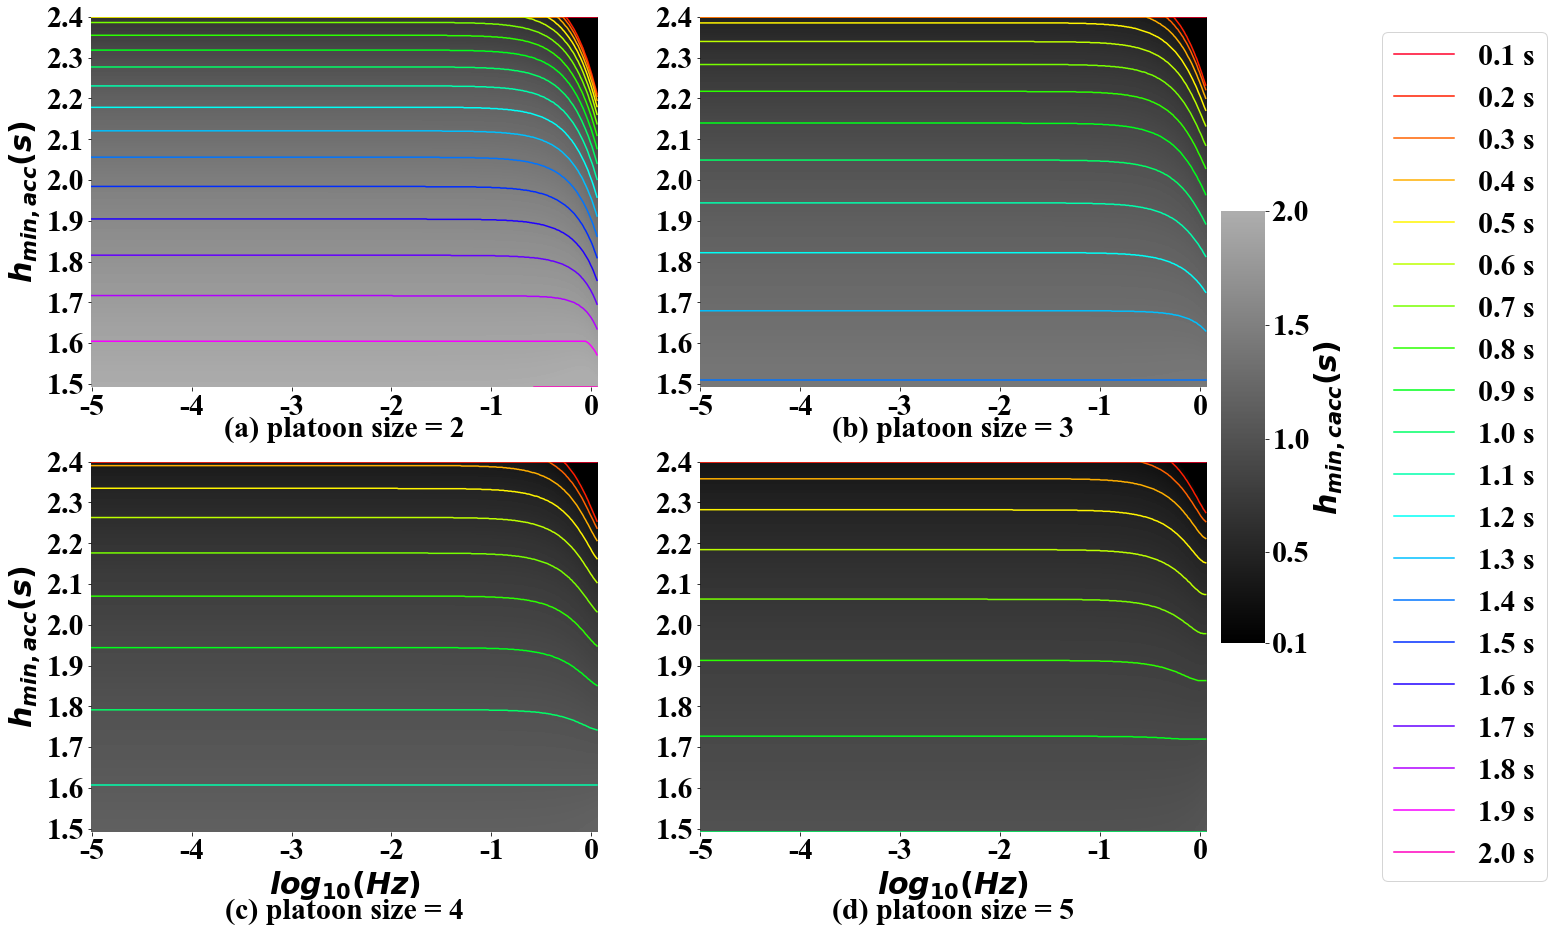
\includegraphics[width=14cm]{figs/fig4.png}
  \caption{~Contour plot of perturbation frequency versus $h_{min,acc}$, indicating the corresponding minimal value for $h_{min,cacc}$.}
  \label{fig4}
\end{figure}

It can be clearly found in Fig.~\ref{fig4}, CACC can maintain a smaller desired time gap with platoon size increasing. Moreover, $h_{min,cacc}$ can significantly decrease with $h_{min,acc}$ increasing, which means the feasibility of eliminating the redundancy within the CACC platoon through the appropriate deployment of the desired time gap. In addition, string stability can be significantly improved as the frequency of perturbation approaches $10^0$ Hz, which is represented as the arc under $10^{-0.5} - 10^0$ Hz in Figure.4. When we focus on the region of $10^{-5} - 10^{-0.5}$ Hz, an interesting phenomenon is discovered that $h_{min,cacc}$ stays the same as the frequency increases, which means the combination of $h_{min,cacc}$ and $h_{min,acc}$ to guarantee the string stability is determined for a specific platoon size.

Based on the conclusions obtained above, in order to maximize the capacity while ensuring string stability and safety, we choose $h_{1,acc}=2s$ and $h_{1,cacc}=0.4s$ for the case of $S=5$ while the desired time gap settings of ACC and CACC for the case of $S=2$ are $h_{0,acc}=2.108s$ and $h_{0,cacc}=0.747s$ in this paper.

\subsection{Analyses of controller switching}
\label{Section 4.2}

For the LV in a CACC platoon, since it cannot communicate with the predecessor vehicle, it loses the information gain from the communication module, so its control system is represented by standard ACC, as shown in Fig.~\ref{fig2} (a).

\subsubsection{Modify ACC controller}
\label{Section 4.2.1}

To incorporate the desired time gap into the controller, the ACC controller in Fig.~\ref{fig2} (a) is reconstructed so that the ACC controller can perform stable interpolation for the different desired time gap $h_i$. And the corresponding equivalent ACC control structure is shown in Fig.~\ref{fig5}. The transfer function of the extended controller is as follows:
\begin{equation}
  K_{e x t, a c c}^{i}(s)=\frac{K_{i}}{1+h_{i} G_{i} K_{i} s}.
\end{equation}
\begin{figure}
  \centering
  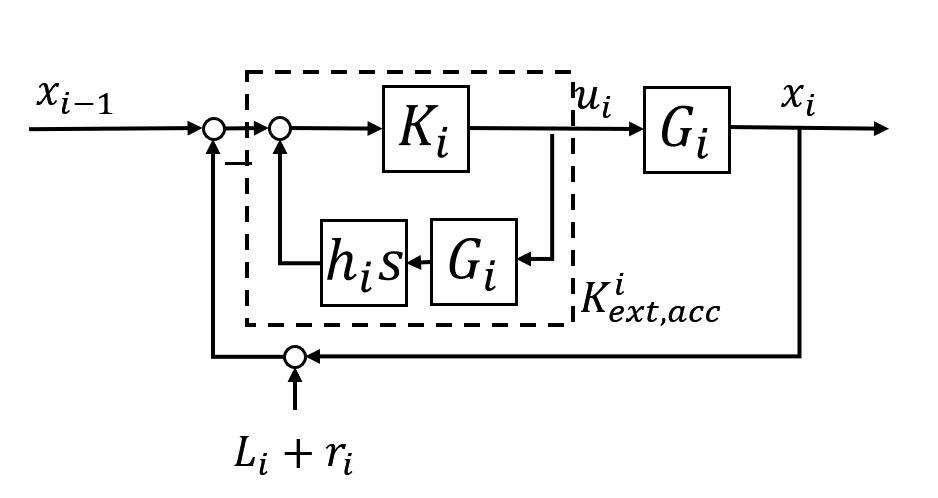
\includegraphics[width=10cm]{figs/fig5.png}
  \caption{~Equivalent ACC control structure.}
  \label{fig5}
\end{figure}

\subsubsection{YK parametrization for ACC controller}
\label{Section 4.2.2}

Based on the mathematical basis introduced in Section~\ref{Section 3.2}, the control structure applied to controller switching needs to be modified accordingly by introducing a dual coprime factor. The control structure for switching based on left coprime factors is shown in Fig.~\ref{fig6}:

\begin{figure}
  \centering
  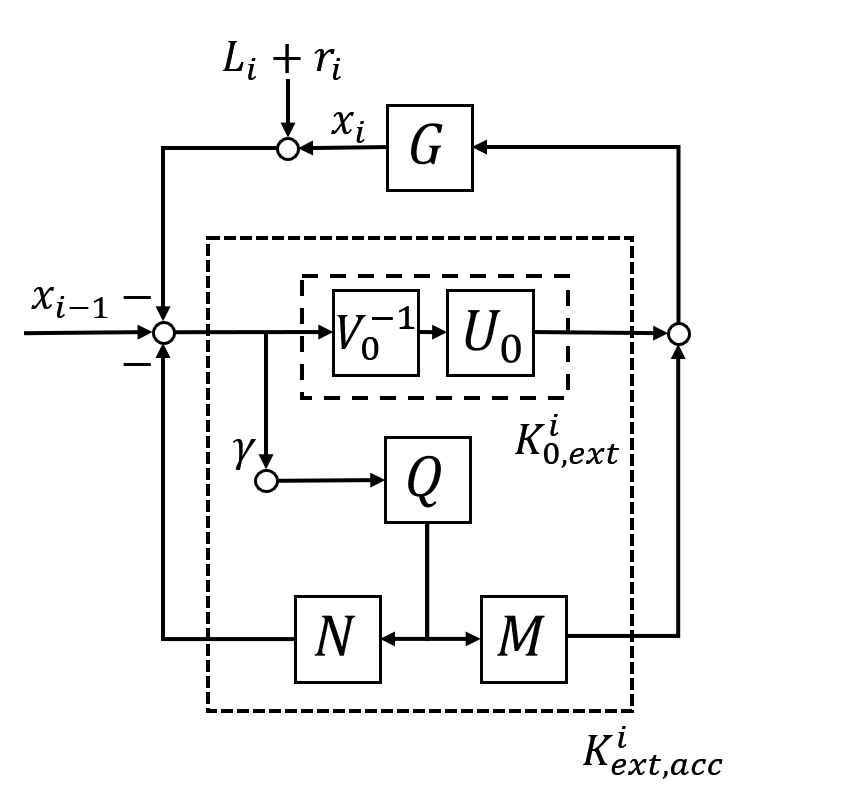
\includegraphics[width=7cm]{figs/fig6.png}
  \caption{~YK control structure for ACC controllers switching.}
  \label{fig6}
\end{figure}
For stable switching purposes, coprime factors need to meet double Bezout's identity as shown in Equation (\ref{Eq16}) based on the state-space matrix of transfer functions of $K_{0,acc}$,$K_{1,acc}$. The specific transfer functions of coprime factors are as follows:
\begin{equation}
  \begin{aligned}
     & U_{0}=\frac{-s(s+1.272)(s+1.8)}{(s+4.42)\left(s^{2}+1.836 s+1.027\right)},                 \\
     & V_{0}=\frac{-4\left(s^{2}+1.902 s+1.135\right)}{(s+4.42)\left(s^{2}+1.836 s+1.027\right)}, \\
     & U_{1}=\frac{-s(s+1.272)(s+1.8)}{(s+4.42)\left(s^{2}+1.808 s+0.9741\right)},                \\
     & V_{1}=\frac{-4\left(s^{2}+1.87 s+1.076\right)}{(s+4.42)\left(s^{2}+1.808 s+0.9741\right)}.
  \end{aligned}
\end{equation}
As for the YK parameter $Q_{acc}$, substitute coprime factors into Equation(\ref{Eq20}):

\begin{equation}
  Q_{a c c}=\frac{-0.1005(s+1.892)(s+4.38)(s+4.42)\left(s^{2}+1.82 s+0.9968\right)\left(s^{2}+1.969 s+1.238\right)}{(s+4.42)^{3}\left(s^{2}+1.808 s+0.9741\right)\left(s^{2}+1.836 s+1.027\right)^{2}}.
\end{equation}

\subsubsection{Modify CACC controller}
\label{Section 4.2.3}

Similar to the method adopted in Section~\ref{Section 4.2.1}, the system construction drawing of the CACC controller is in Figure.~\ref{fig3}, which is reconstructed to incorporate the desired time gap $h_i$ into the controller. And the corresponding equivalent CACC control structure is shown in Figure.~\ref{fig7}. The transfer function of the extended controller is as follows:

\begin{equation}
  K_{e x t, c a c c}^{i}(s)=\frac{K_{i}}{1+h_{i} G_{i} K_{i} s}.
\end{equation}

\begin{figure}
  \centering
  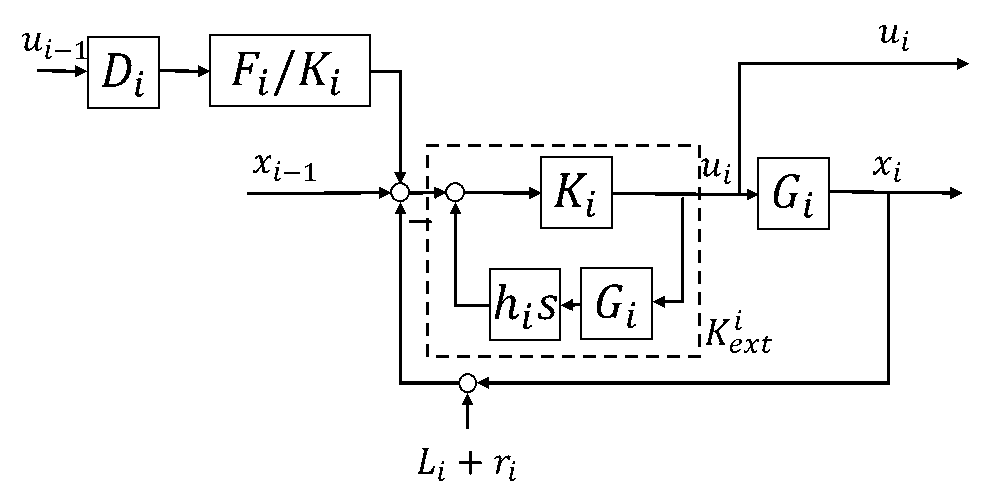
\includegraphics[width=10cm]{figs/fig7.png}
  \caption{~Equivalent CACC control structure.}
  \label{fig7}
\end{figure}

\subsubsection{YK parametrization for CACC controller}
\label{Section 4.2.4}

Similar to Section~\ref{Section 4.2.2}, the control structure applied to controller switching needs to be modified accordingly by introducing a dual coprime factor based on the mathematical basis presented in Section~\ref{Section 3.2}. The control structure for switching based on left coprime factors is shown in Figure.~\ref{fig8}:

\begin{figure}
  \centering
  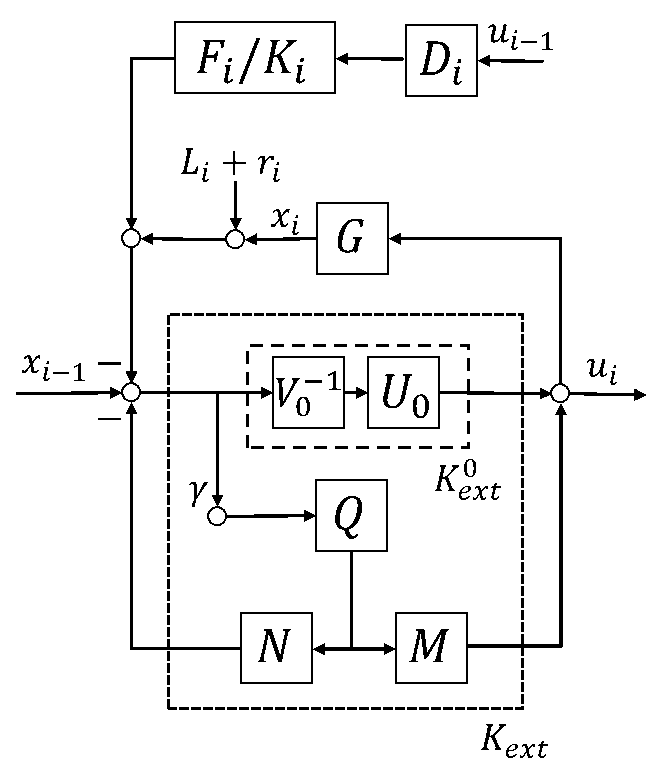
\includegraphics[width=7cm]{figs/fig8.png}
  \caption{~YK control structure for CACC controllers switching.}
  \label{fig8}
\end{figure}

Based on Equation (\ref{Eq17}-\ref{Eq18}), coprime factors which meet double Bezout's identity as shown in Equation (\ref{Eq16}) can be obtained easily. The specific transfer functions of coprime factors are as follows:
\begin{equation}
  \begin{aligned}
     & U_{3}=\frac{-s(s+1.272)(s+1.8)}{(s+4.406)(s+1.159)(s+0.3148)},    \\
     & V_{3}=\frac{-4(s+1.144)(s+0.3515)}{(s+4.406)(s+1.159)(s+0.3148)}, \\
     & U_{4}=\frac{-s(s+1.272)(s+1.8)}{(s+4.397)(s+1.226)(s+0.1438)},    \\
     & V_{4}=\frac{-4(s+1.221)(s+0.1587)}{(s+4.397)(s+1.226)(s+0.1438)}.
  \end{aligned}
\end{equation}
As for the YK parameter $Q_{cacc}$, substitute coprime factors into Equation(\ref{Eq20}):
\begin{small}
  \begin{equation}
    Q_{c a c c}=\frac{-0.4451(s+4.402)(s+3.51)(s+1.918)(s+1.8)(s+1.274)(s+1.219)(s+1.414)(s+0.3596)(s+0.1572)}{(s+4.397)(s+1.8)(s+1.272)(s+1.226)(s+0.1438)(s+4.406)^{2}(s+0.3148)^{2}\left(s^{2}+2.319 s+1.344\right)}.
  \end{equation}
\end{small}

\subsection{Tuning function $\gamma$ for CACC platoon}
\label{Section 4.3}

The theoretical results of Section~\ref{Section 4.1} point out that different CACC platoon sizes have different combinations of $h_{min,acc}$ and $h_{min,cacc}$ as string stability margin. To avoid being restricted by the platoon size, a corresponding tuning function $\gamma$ for the platoon size is required so that CACPC can be applied under different platoon sizes.

The theoretical results of Section~\ref{Section 4.1} indicate that different CACC platoon sizes have different combinations of $h_{min,acc}$ and $h_{min,cacc}$ as string stability margin. In order to avoid being restricted by the platoon size, the corresponding tuning function $\gamma$ about platoon size is required so that CACPC can be applied under different platoon sizes. Based on the reasons above, a numerical analysis is conducted to obtain the combination of $\gamma_{acc}$ and $\gamma_{cacc}$ which can maintain string stability of CACC platoon under different platoon sizes. The results are shown in Figure.~\ref{fig9}, where the transparent gray plane and the curve on it represent the string stability margin plane and the intersection of the string stability margin plane and the amplitude surface. It is worth noting that Figure.~\ref{fig9} is carried out at the frequency of $10^{-5}$ Hz and further exploration that covers a broader frequency domain is carried out in Section~\ref{Section 5.1}.

\begin{figure}
  \centering
  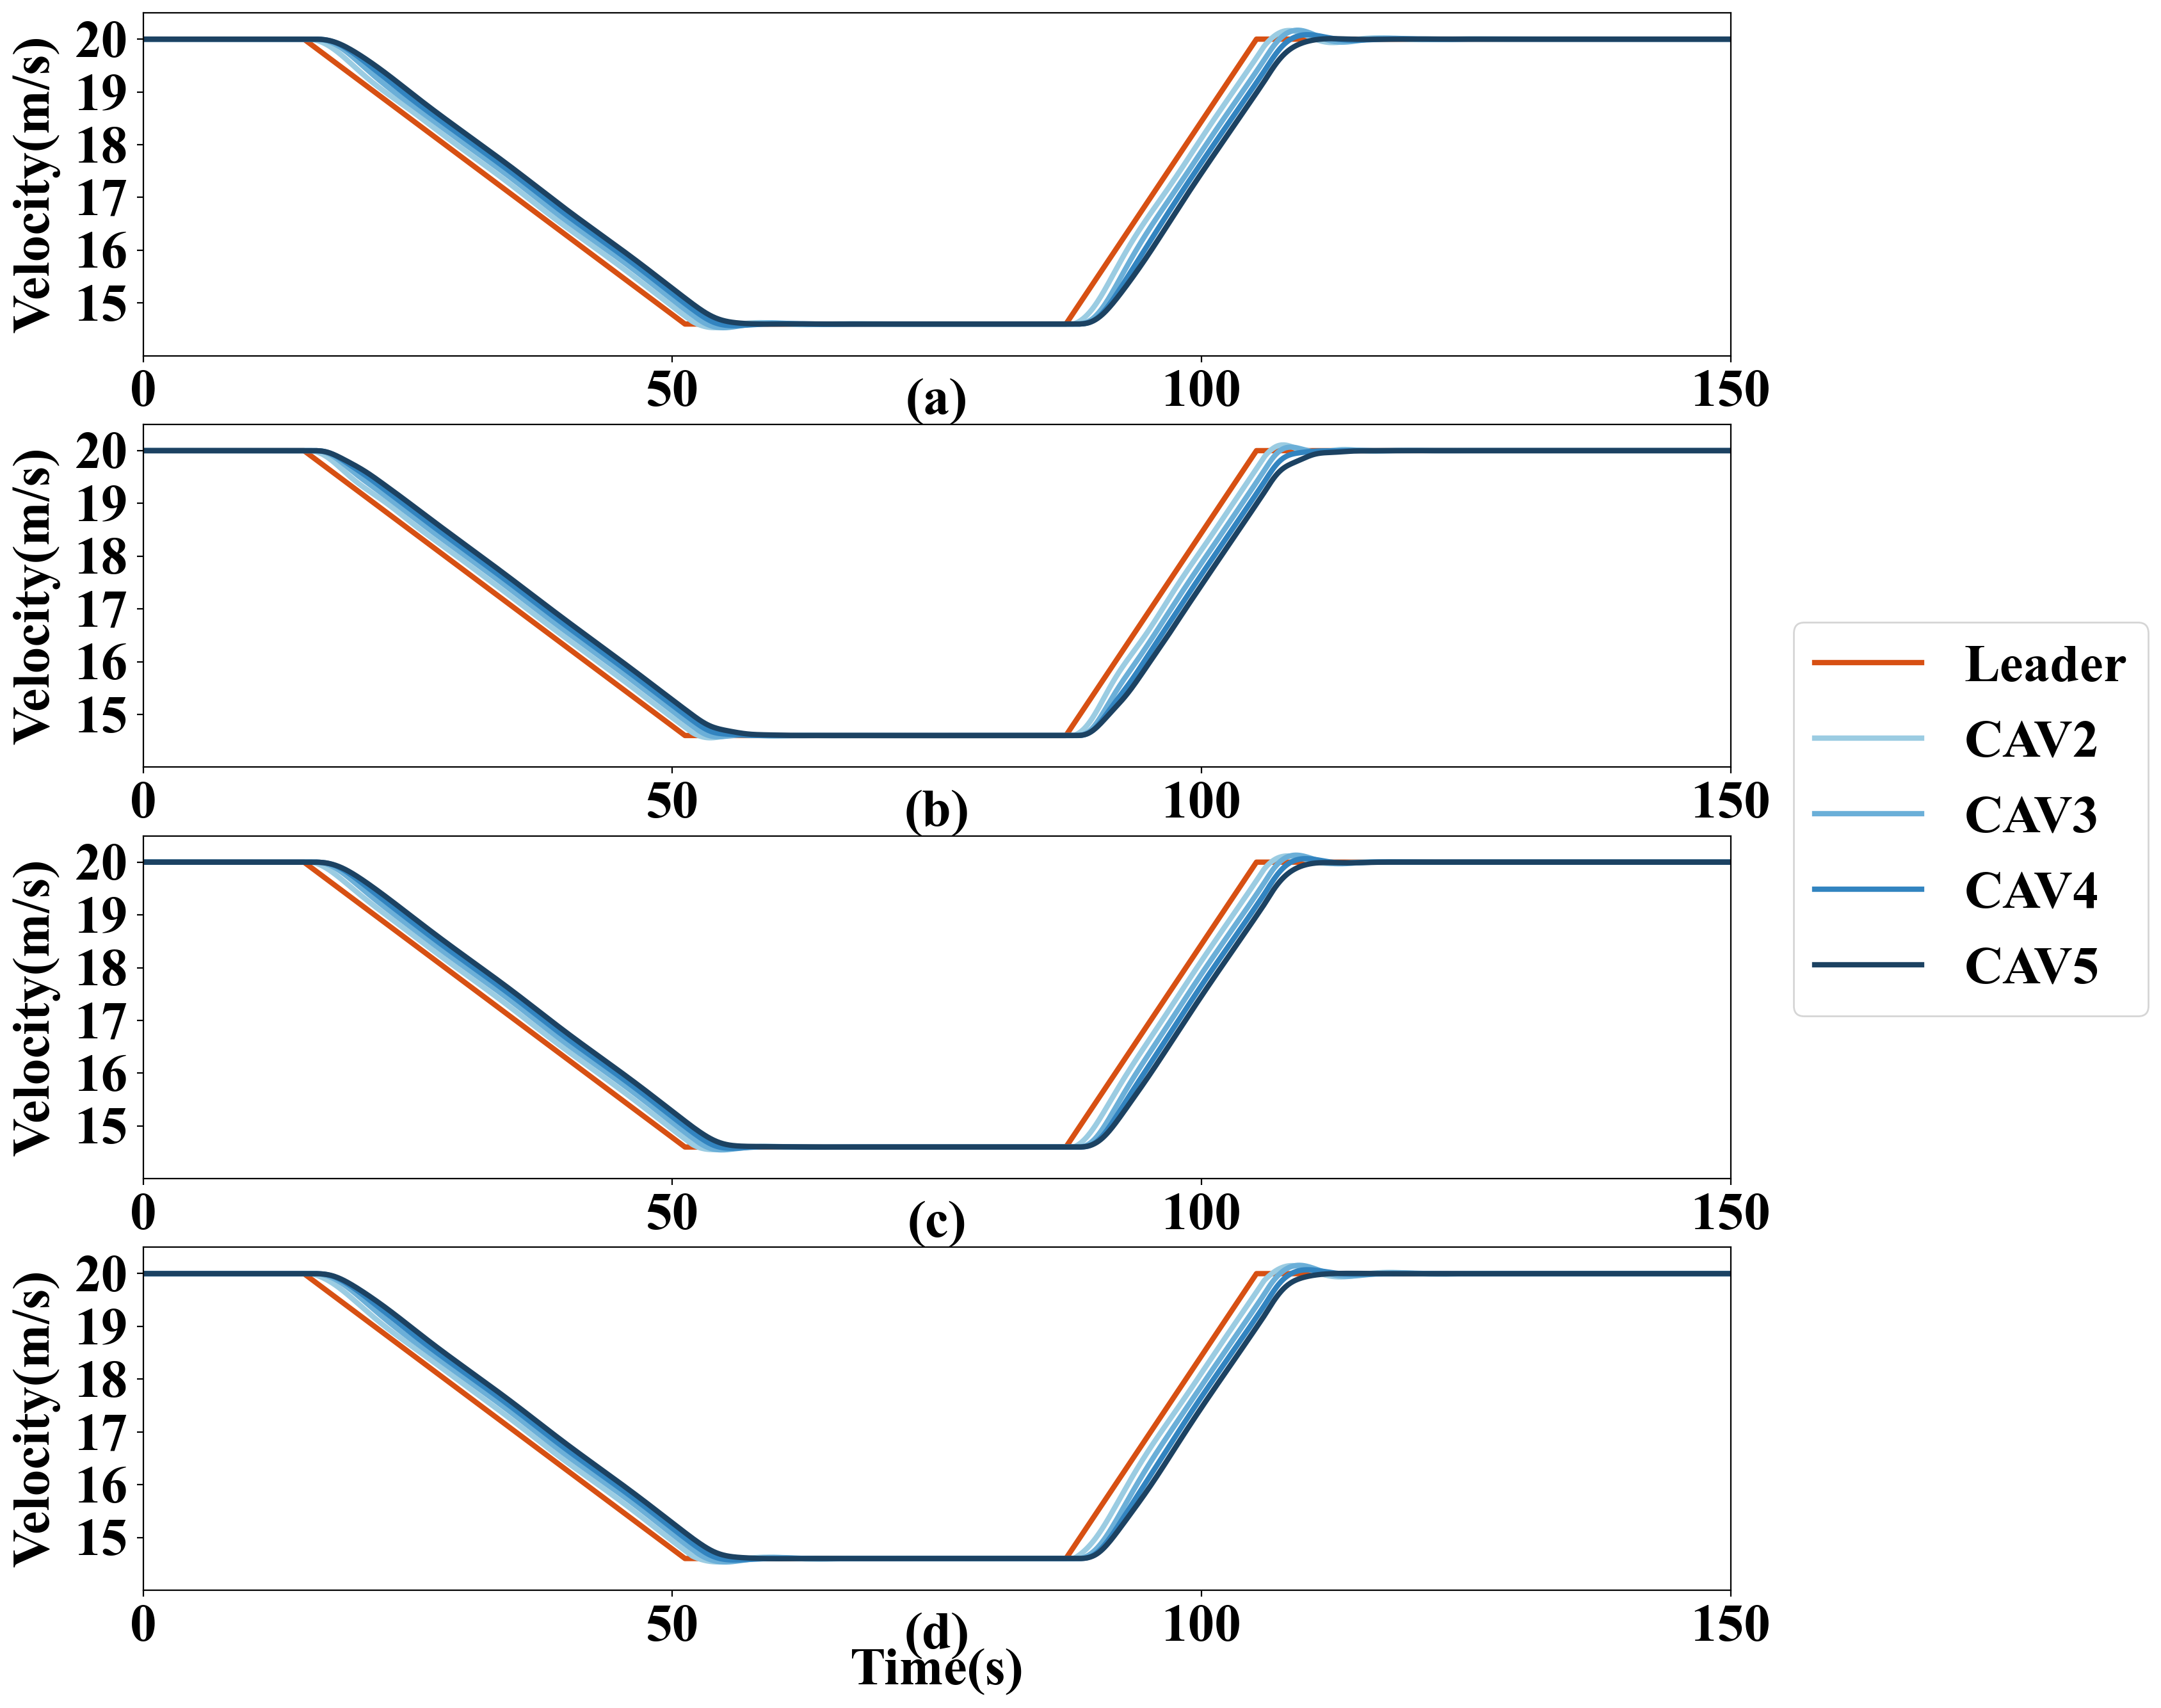
\includegraphics[width=14cm]{figs/fig9.png}
  \caption{~String stability's surface depending on YK $\gamma_{acc}$ and $\gamma_{cacc}$.}
  \label{fig9}
\end{figure}
We can conclude from Figure.~\ref{fig9} that the intersection of the transparent plane and string stability's surface is the basis for selecting $\gamma_{acc}$ and $\gamma_{cacc}$, which can ensure string stability and tap the advantages of CACPC as much as possible. Through the curve-fitting method, we can get the expression of the intersection as follows (since any $\gamma$ can meet the string stability at platoon size = 5, there is no corresponding expression.):
\begin{equation}
  \gamma_{c a c c}= \begin{cases}-0.0501 * \gamma_{a c c}+0.2221 ,& \text { if } n=2 \\ -0.0248 * \gamma_{a c c}+0.5815 ,& \text { if } n=3 \\ -0.0165 * \gamma_{a c c}+0.8995 ,& \text { if } n=4\end{cases}.
\end{equation}
Considering the gain-scheduling method, the appropriate tuning function $\gamma$ is derived based on the expression above:
\begin{equation}
  \gamma_{a c c}=\left\{\begin{array}{cc}
    0 ,   & \text { if } n=1 \\
    0.4 , & \text { if } n=2 \\
    0.7 , & \text { if } n=3 \\
    0.9 , & \text { if } n=4 \\
    1 ,   & \text { if } n=5
  \end{array}\right.,
\end{equation}
\begin{equation}
  \gamma_{c a c c}=\left\{\begin{array}{cc}
    0 ,   & \text { if } n=1 \\
    0.3 , & \text { if } n=2 \\
    0.6 , & \text { if } n=3 \\
    0.9 , & \text { if } n=4 \\
    1 ,   & \text { if } n=5
  \end{array}\right.,
\end{equation}
where, $n$ denotes platoon size.

\section{Numerical analyses}
\label{Section 5}

In this section, we first validate the string stability of CACPC based on the theoretical result derived in Section~\ref{Section 4} by numerical simulation. Then a series of simulation experiments are conducted to explore the impact of YK parameterization on dynamic performance.

\subsection{Validation of string stability}
\label{Section 5.1}

\begin{figure}
  \centering
  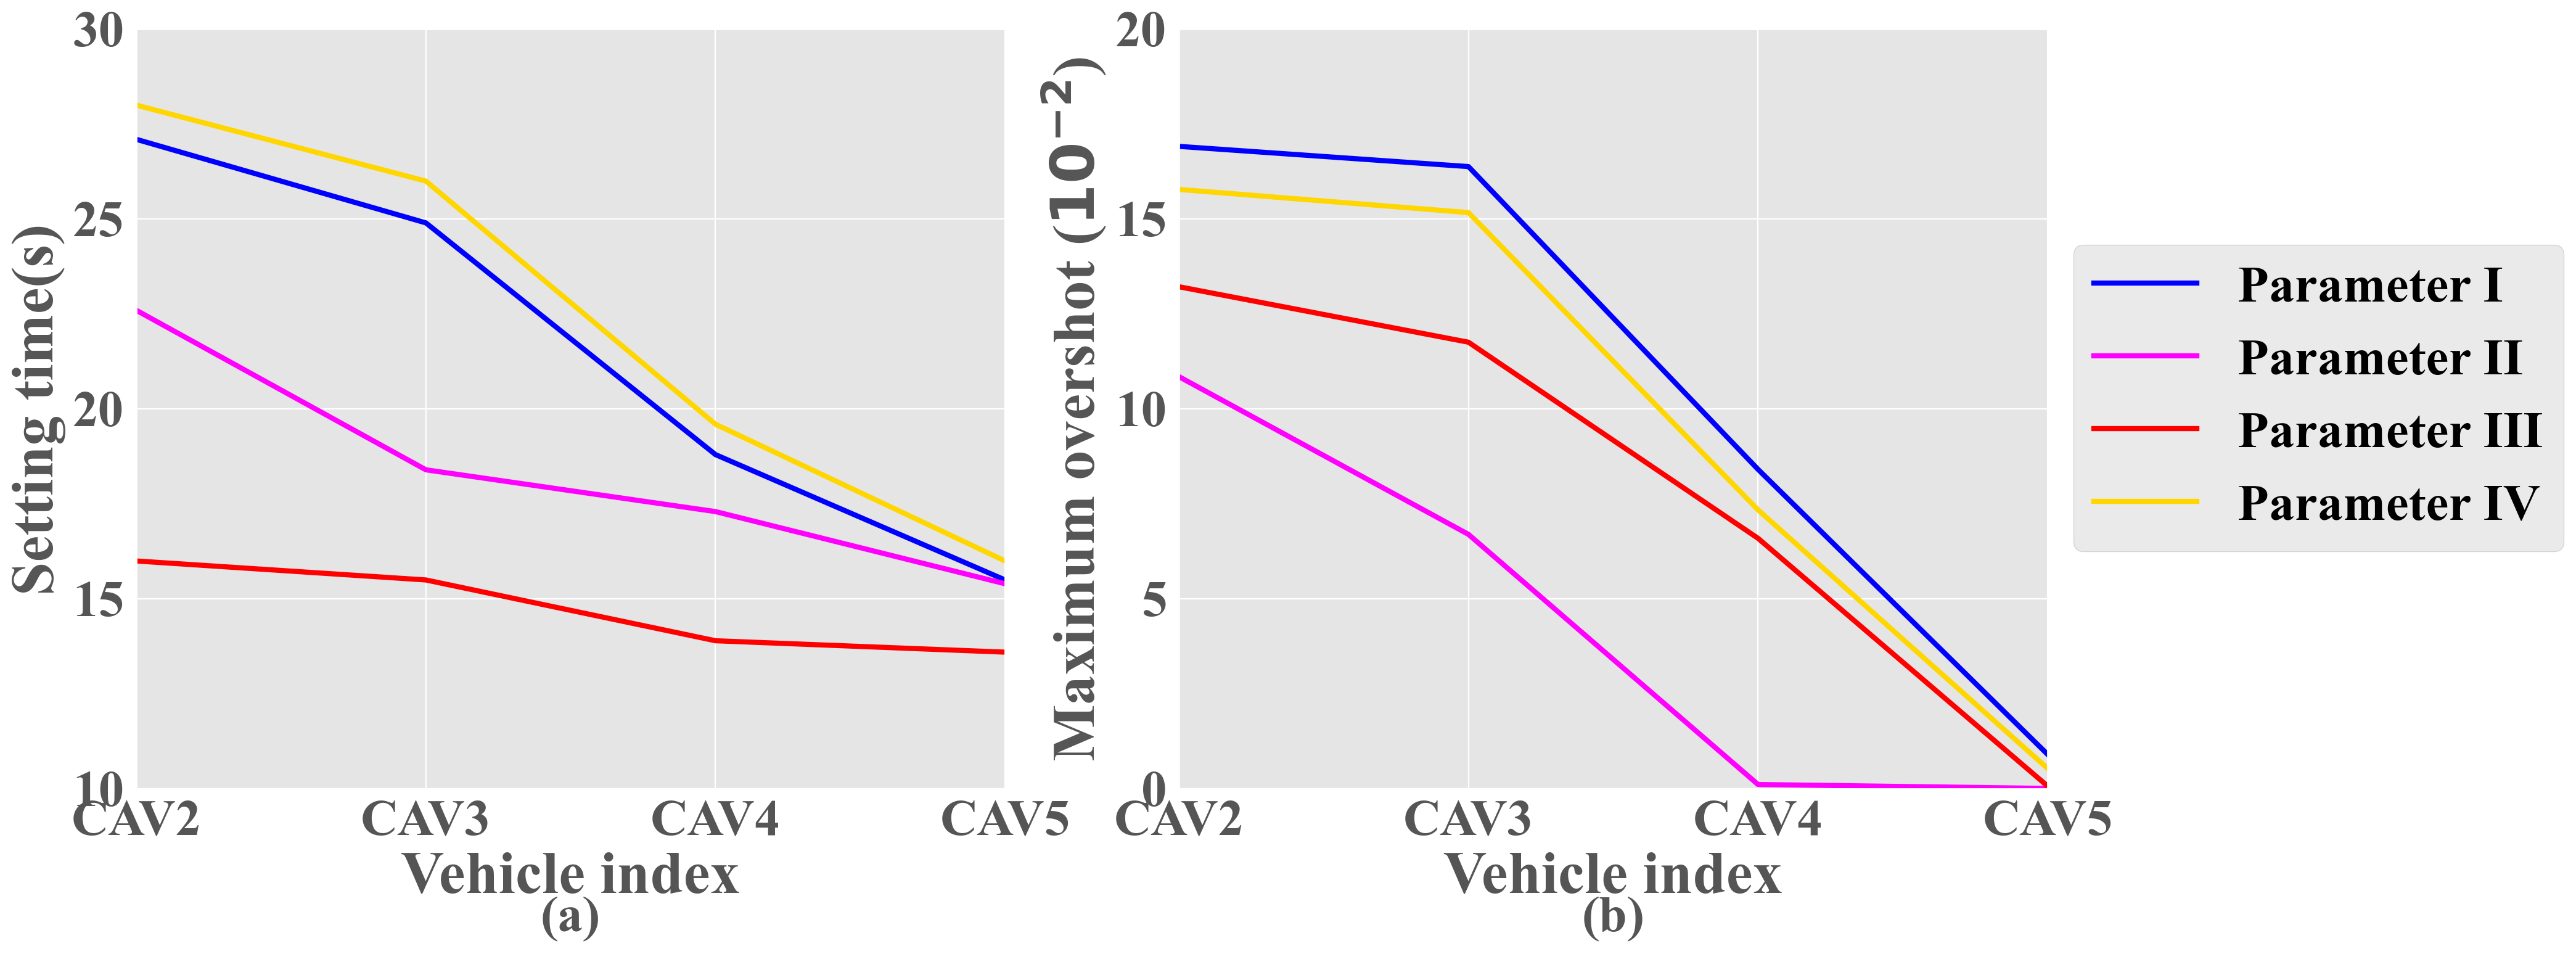
\includegraphics[width=14cm]{figs/fig10.png}
  \caption{~String stability's surface depending on platoon size.}
  \label{fig10}
\end{figure}

Based on the results in Section~\ref{Section 4.2} and ~\ref{Section 4.3}, we have obtained the amplitude of CACPC under different platoon sizes. It is necessary to keep the string stable to prevent the perturbation from being amplified during propagation. Therefore, a numerical experiment is conducted to explore the string stability of CACC platoon under low frequency ($10^{-5} - 10^0$ Hz). Figure.~\ref{fig10} shows the result where the curved surface represents the amplitude of the CACC platoon under low frequency ($10^{-5} - 10^0$ Hz) and different platoon sizes.

Figure.~\ref{fig10} indicates that the CACPC proposed above can avoid amplifying perturbation which means it can maintain string stability during the switching process.

\subsection{Simulation experiments of YK parameterization}
\label{Section 5.2}

Behaviors observed in simulation experiments are closer to those in the real traffic environment compared to theoretical analyses. In order to further explore the actual effect of the controller switching using the YK parameterization, a series of simulation experiments are carried out based on CACPC as a supplement to the theoretical analysis.

\subsubsection{Simulation experiments maintain a constant speed during the forming and splitting process}
\label{Section 5.2.1}

\textit{Simulation scenario:} The simulation scenario is set as: at first, a leader vehicle drives on an infinitely long road under a given speed and acceleration configuration(containing five same small perturbations that occurred at the simulation time of 300s, 1000s, 1700s, 2400s, and 3100s under different platoon size). There are four experiments conducted:
\begin{enumerate}
  \item \textit{Experiment one:} The forming process of the CACC platoon with YK parameterization where an ACC (which is a CACC but degraded to an ACC functionally) follows the leader at the beginning, and more CACCs join the CACC platoon one by one at the simulation time of 700s, 1400s, 2100s, and 2800s.
  \item \textit{Experiment two:} The forming process of the CACC platoon without YK parameterization where an ACC (which is a CACC but degraded to an ACC functionally) follows the leader at the beginning, and more CACCs join the CACC platoon one by one at the simulation time of 700s, 1400s, 2100s, and 2800s.
  \item \textit{Experiment three:} The splitting process of the CACC platoon with YK parameterization where an ACC (which is a CACC but degraded to an ACC functionally) follows the leader at the beginning, and more CACCs join the CACC platoon one by one at the simulation time of 700s, 1400s, 2100s, and 2800s.
  \item \textit{Experiment four:} The splitting process of the CACC platoon without YK parameterization where an ACC (which is a CACC but degraded to an ACC functionally) and four CACCs follow the leader at the beginning, and the last CACC in the platoon leaves one by one at the simulation time of 700s, 1400s, 2100s, and 2800s.
\end{enumerate}
The first pair of experiments is the forming process of the CACC platoon where an ACC (which is a CACC but degraded to an ACC functionally) follows the leader at the beginning, and more CACCs join the CACC platoon one by one at the simulation time of 700s, 1400s, 2100s, and 2800s. Moreover, periodic perturbations are applied to the leader to explore the string stability of the CACC platoon under different platoon size. Another pair of experiments are conducted simulating the splitting process of the CACC platoon. It should be noted that there are total four experiments conducted to analyze the impact of the YK parameterization under the platoon forming case and the platoon splitting case. Experiment one and three applies YK parameterization with tuning function $\gamma$ proposed above, while experiment two and four switches to CACPC mode directly only the platoon size reaches maximum platoon size $S=5$. Furthermore,

\begin{figure}
  \centering
  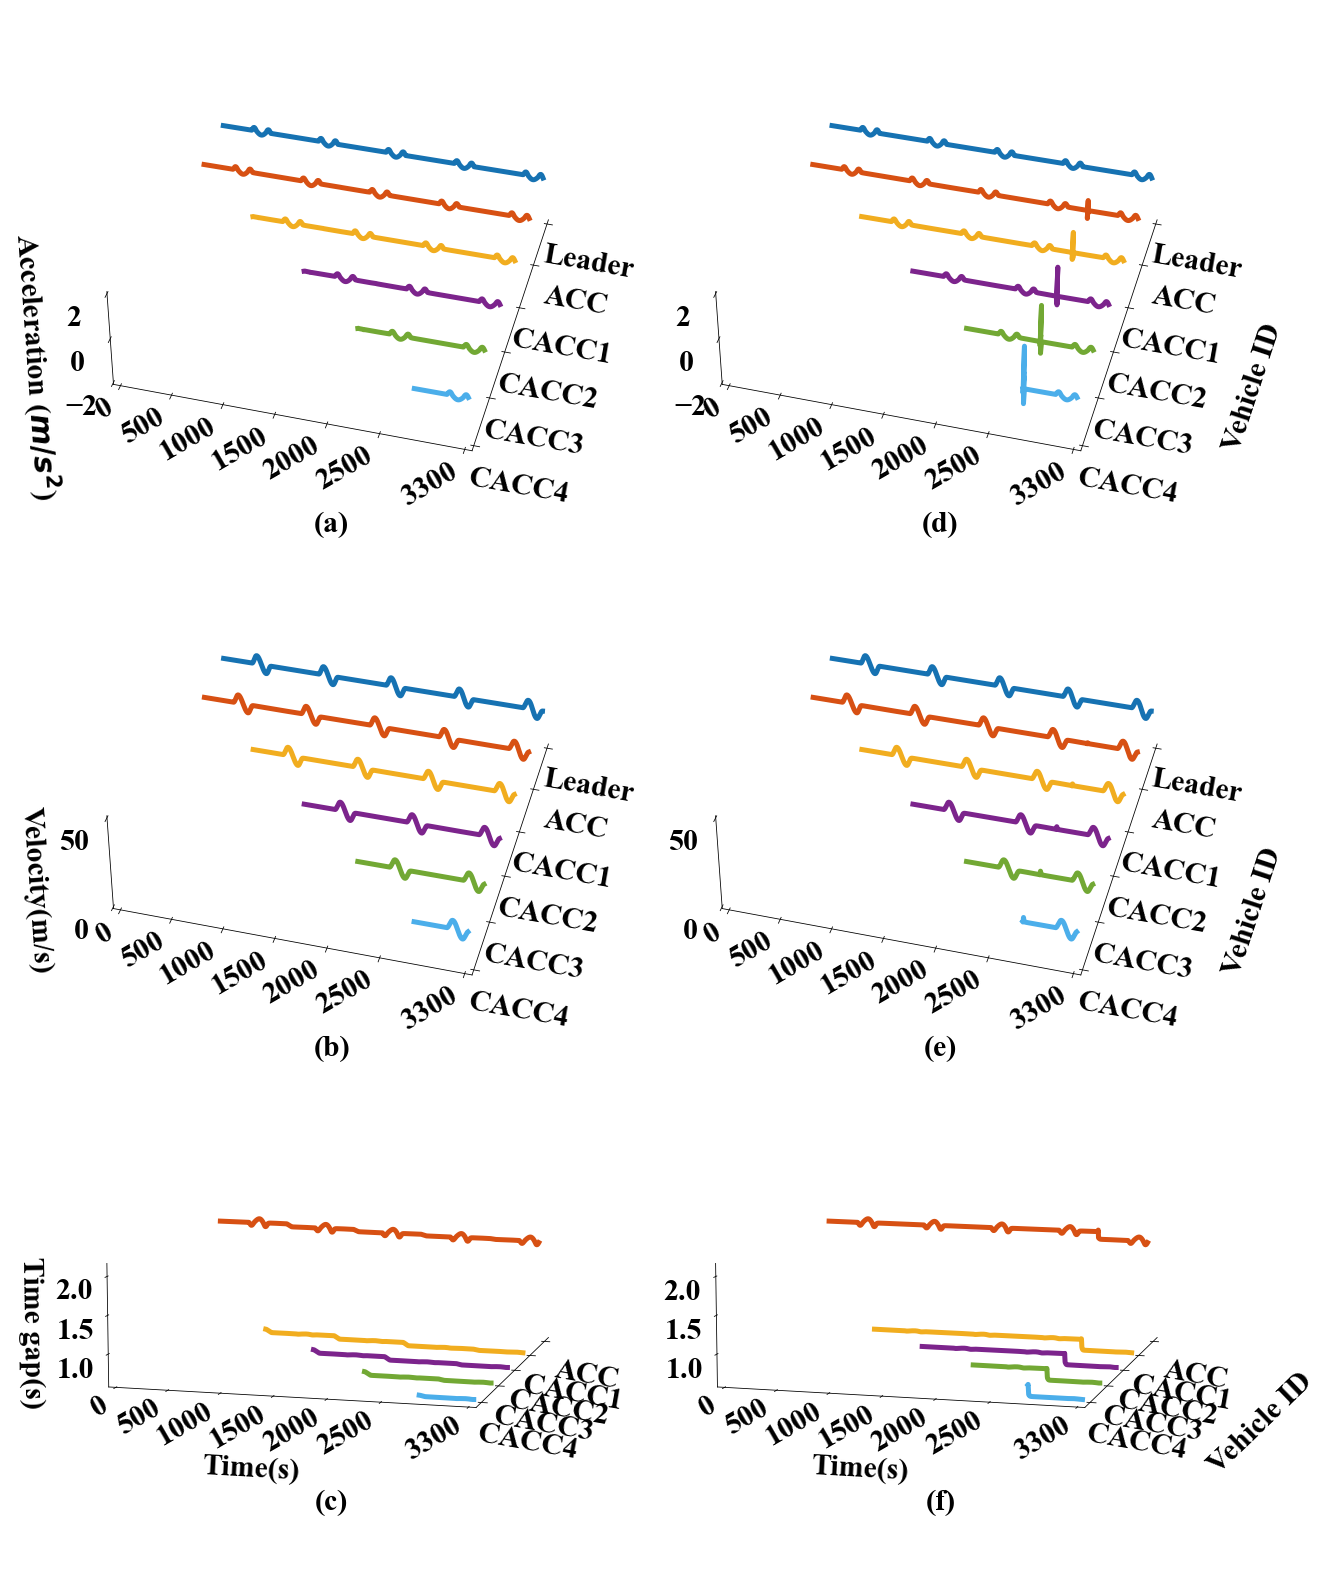
\includegraphics[width=14cm]{figs/c_form.png}
  \caption{~Simulation results of experiment one and two: CACPC with or without YK parameterization under the platoon forming case. (a)-(c) show the simulation results of experiment one and (d)-(f) show the simulation results of experiment two. (a),(d) Acceleration of simulation results; (b),(e) Velocity of simulation results; (c),(f) Time gap of simulation results.}
  \label{new1}
\end{figure}

\begin{figure}
  \centering
  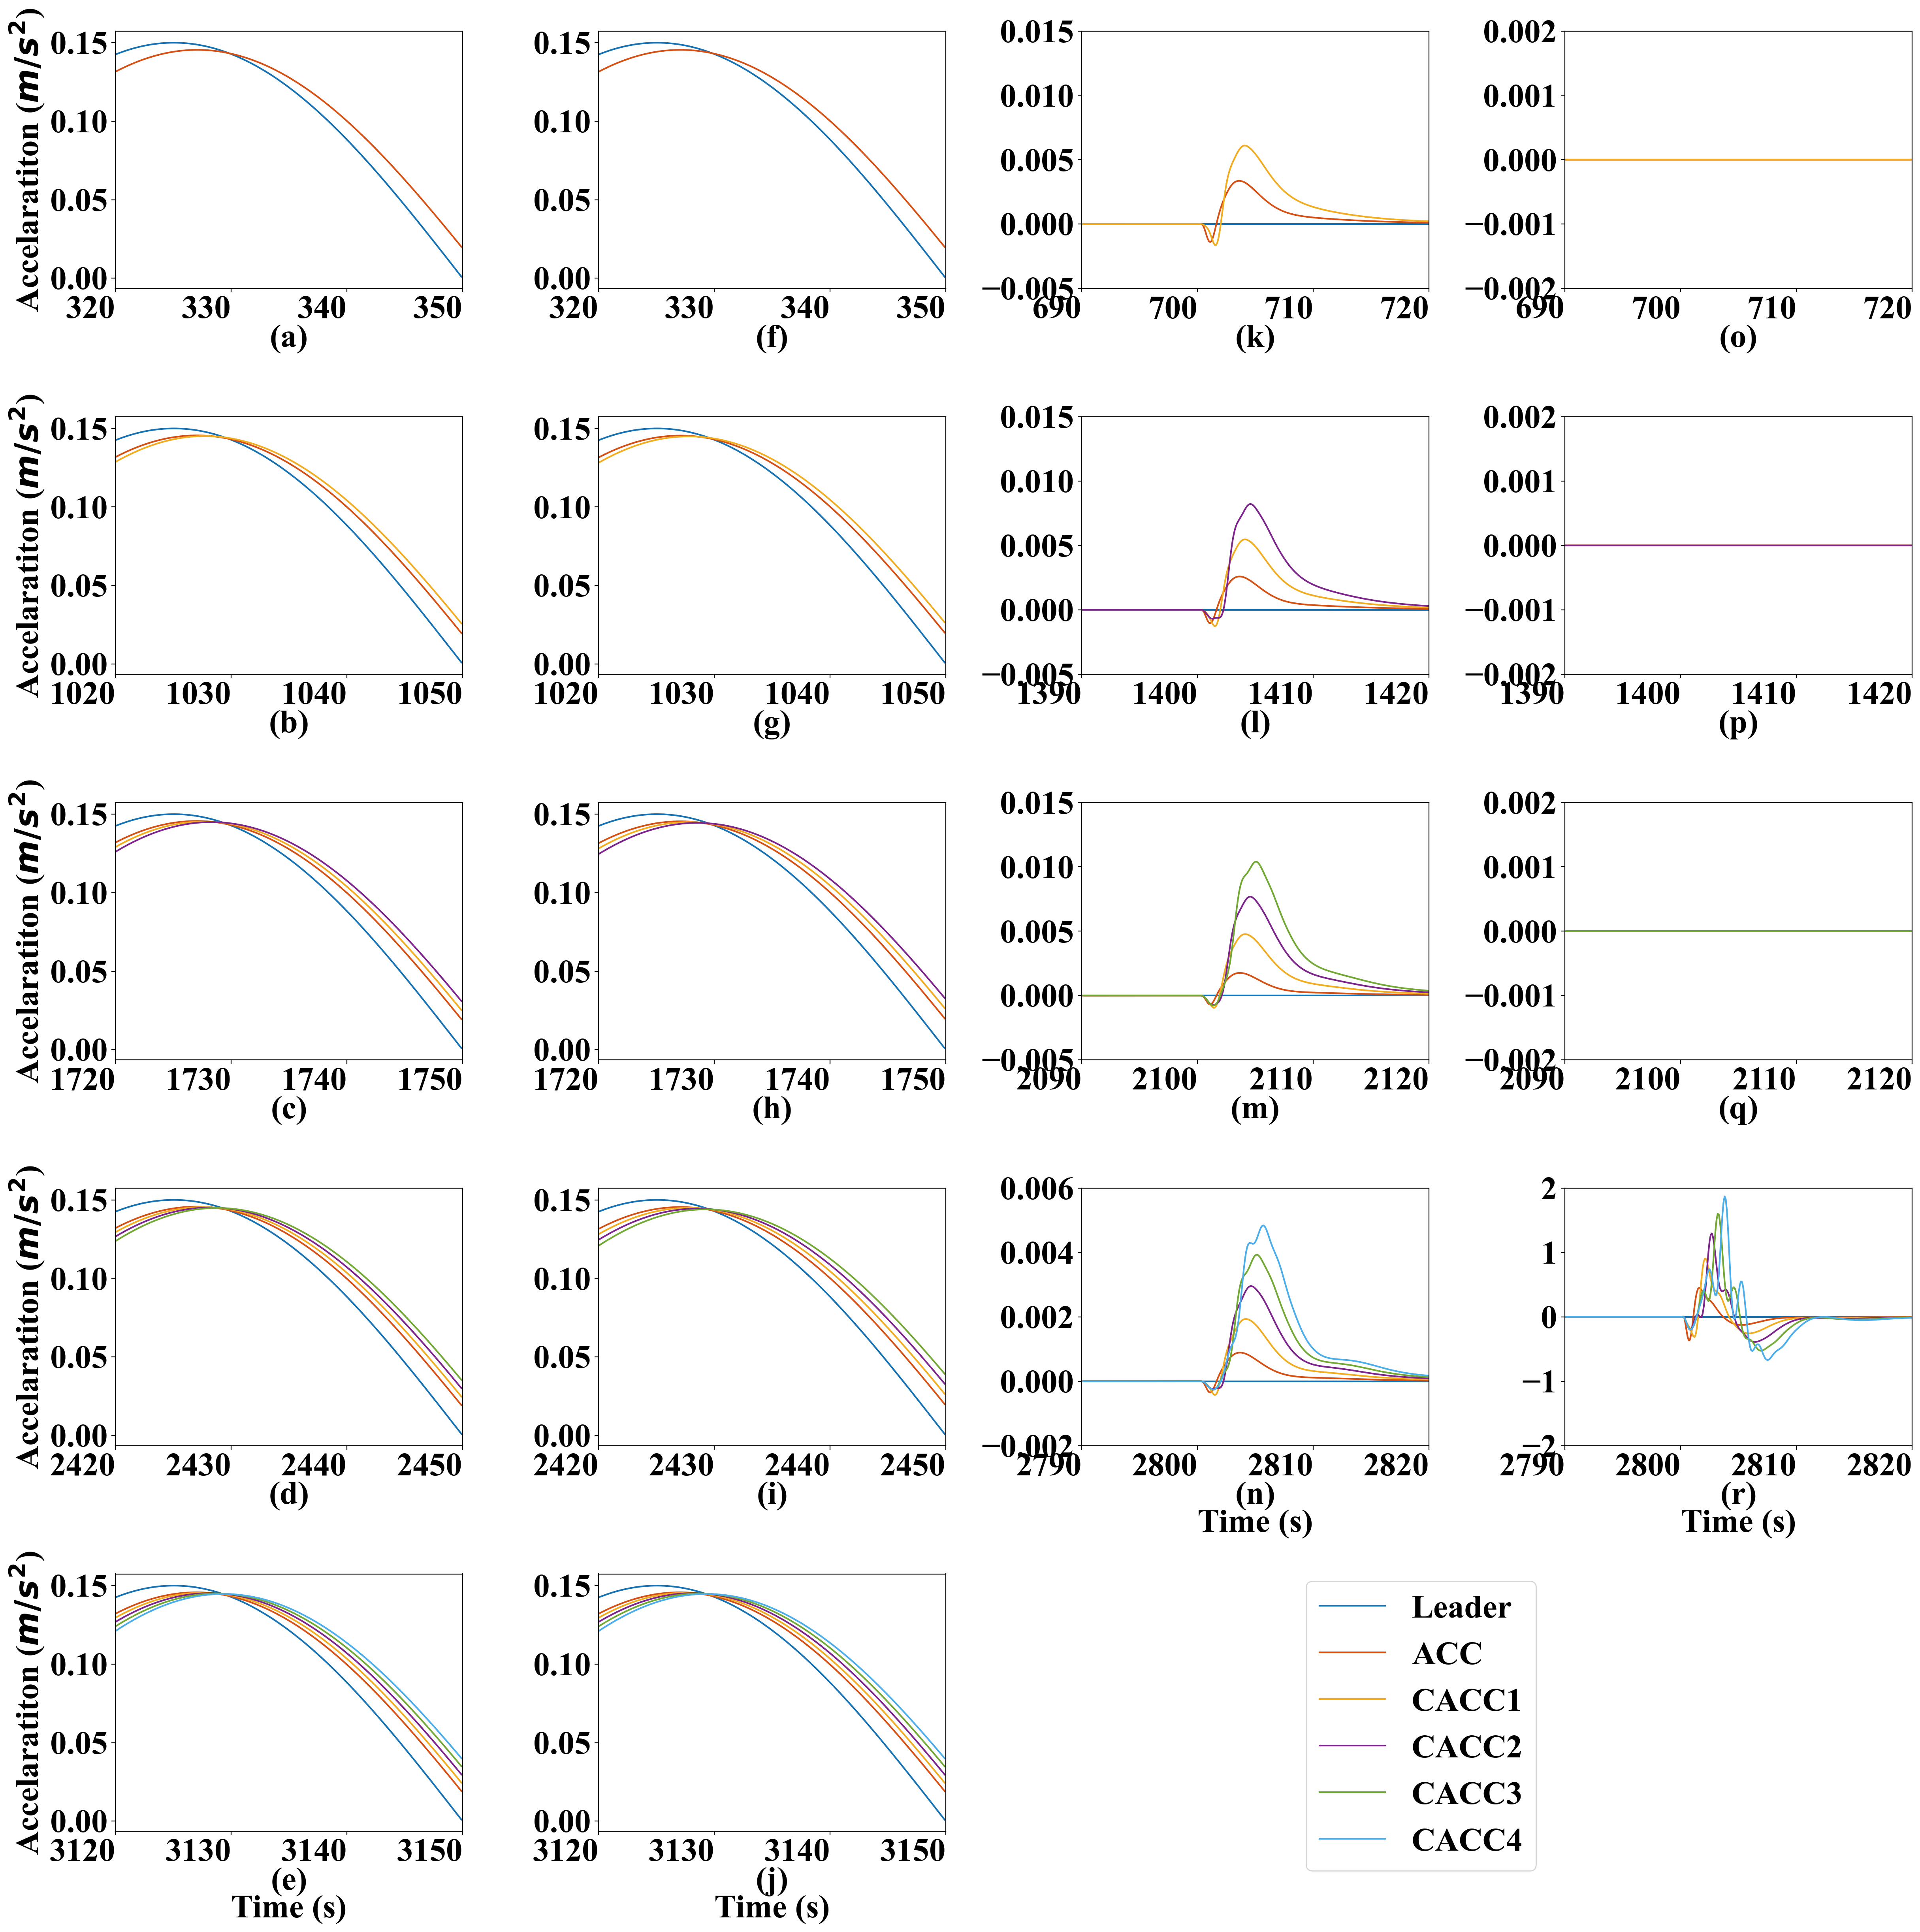
\includegraphics[width=14cm]{figs/form_detail.png}
  \caption{~Detailed perturbation simulation results of experiment one and two: CACPC with or without YK parameterization under the platoon forming case. For experiment one, (a)-(e) show the propagating processes of five applied perturbations and (k)-(n) show the four switching processes. For experiment two, (f)-(j) show the propagating processes of five applied perturbations and (o)-(r) show the four switching processes.}
  \label{new2}
\end{figure}

\begin{figure}
  \centering
  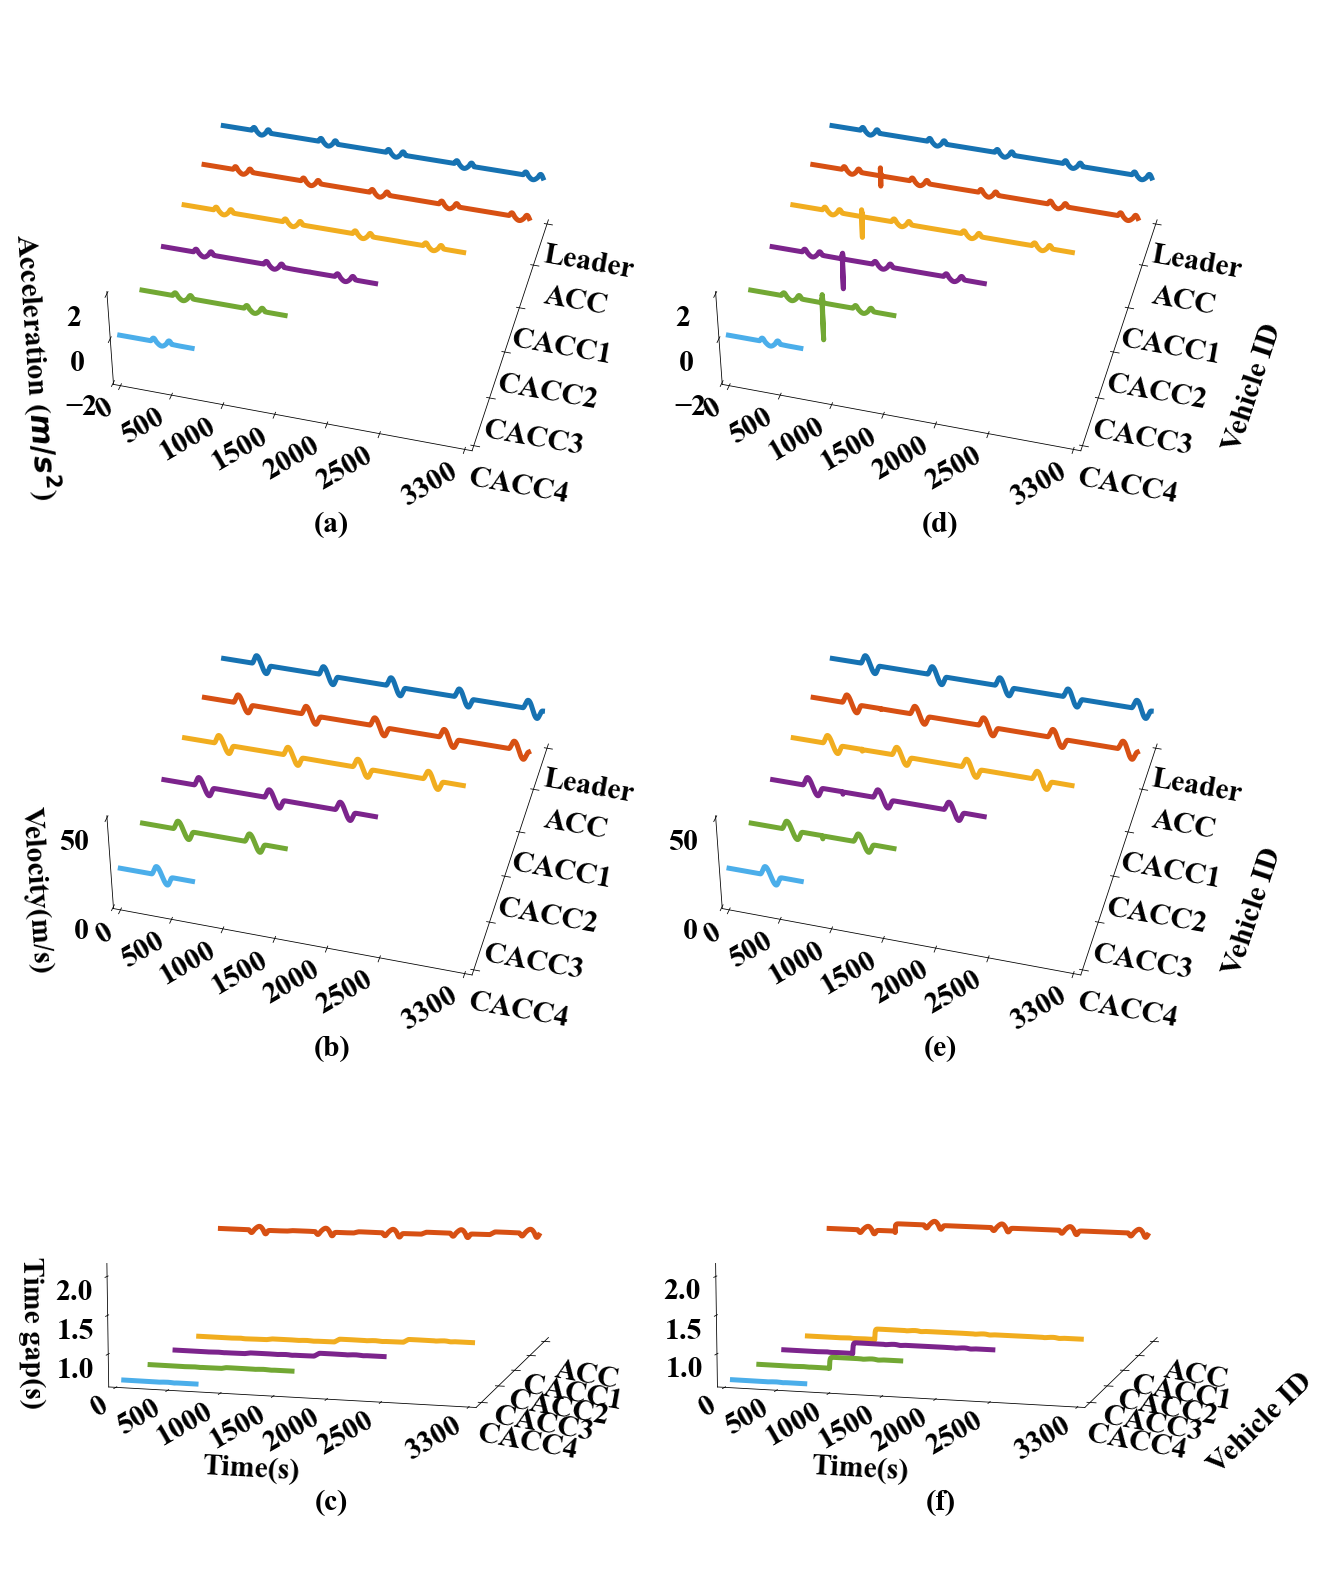
\includegraphics[width=14cm]{figs/c_split.png}
  \caption{~Simulation results of experiment three and four: CACPC with or without YK parameterization under the platoon splitting case. (a)-(c) show the simulation results of experiment three and (d)-(f) show the simulation results of experiment four. (a),(d) Acceleration of simulation results; (b),(e) Velocity of simulation results; (c),(f) Time gap of simulation results.}
  \label{new3}
\end{figure}

\begin{figure}
  \centering
  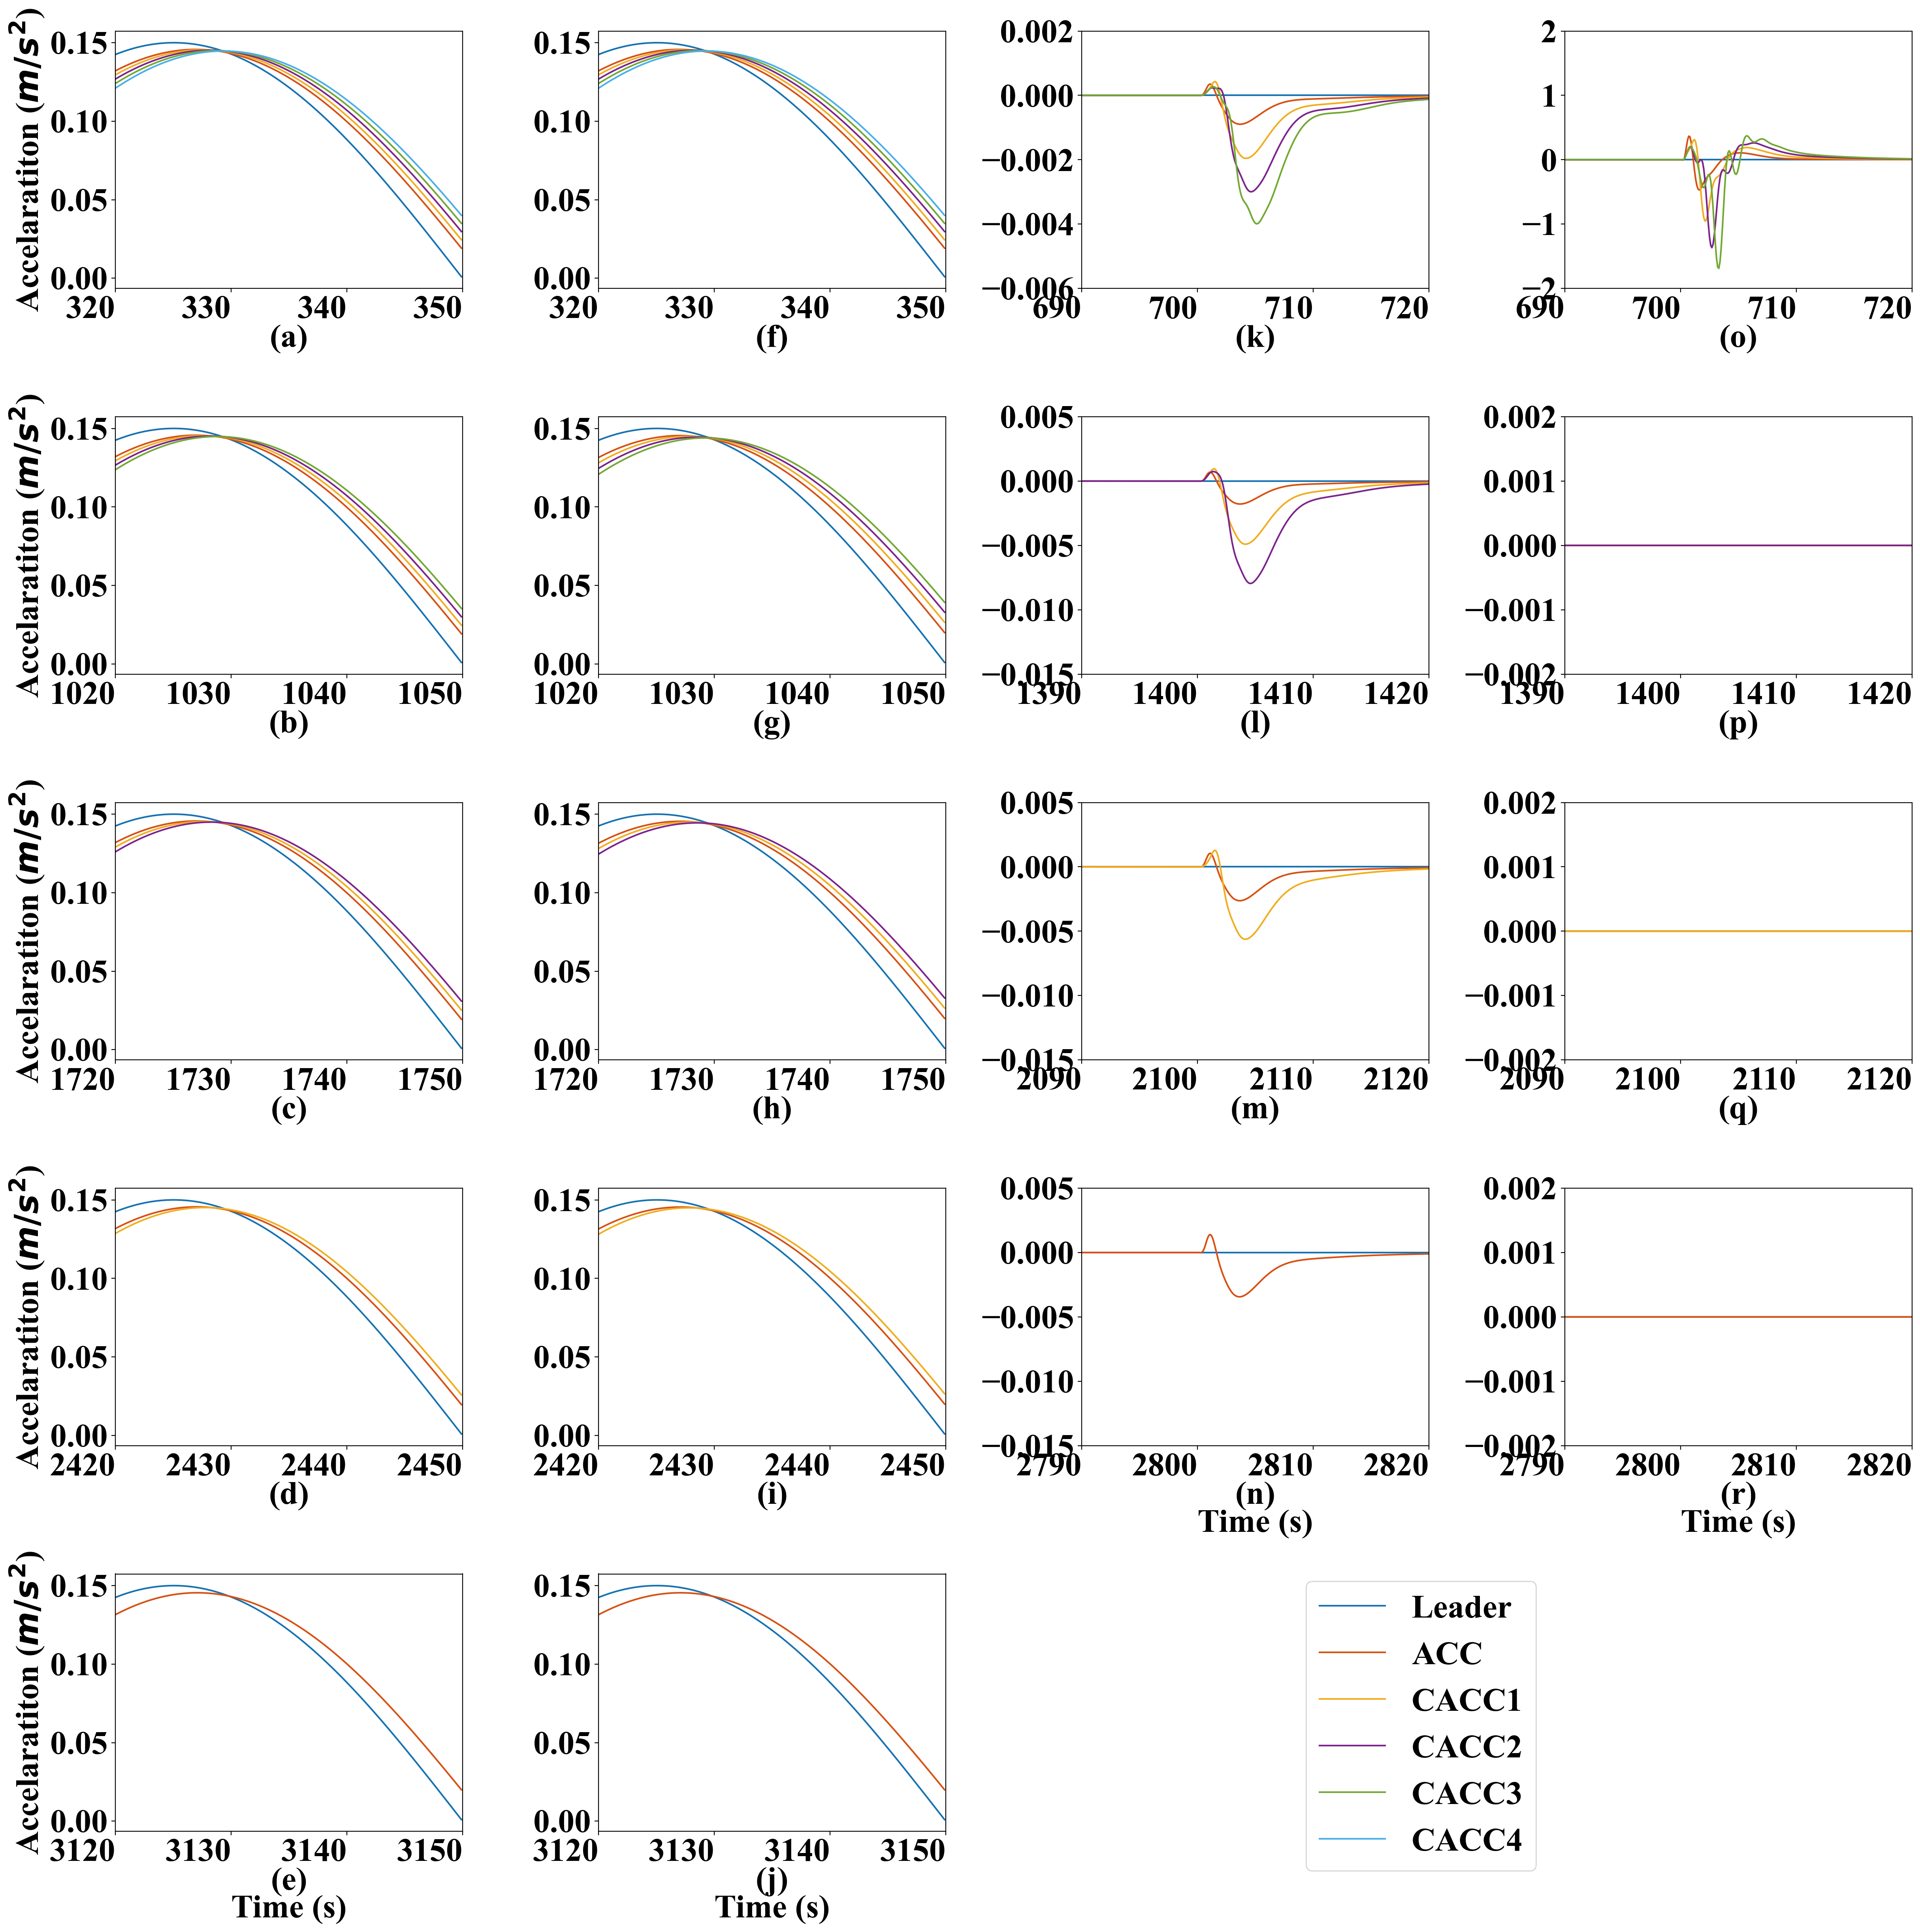
\includegraphics[width=14cm]{figs/split_detail.png}
  \caption{~Detailed perturbation simulation results of experiment three and four: CACPC with or without YK parameterization under the platoon splitting case. For experiment three, (a)-(e) show the propagating processes of five applied perturbations and (k)-(n) show the four switching processes. For experiment four, (f)-(j) show the propagating processes of five applied perturbations and (o)-(r) show the four switching processes.}
  \label{new4}
\end{figure}

% \begin{figure}
% 	\centering
% 		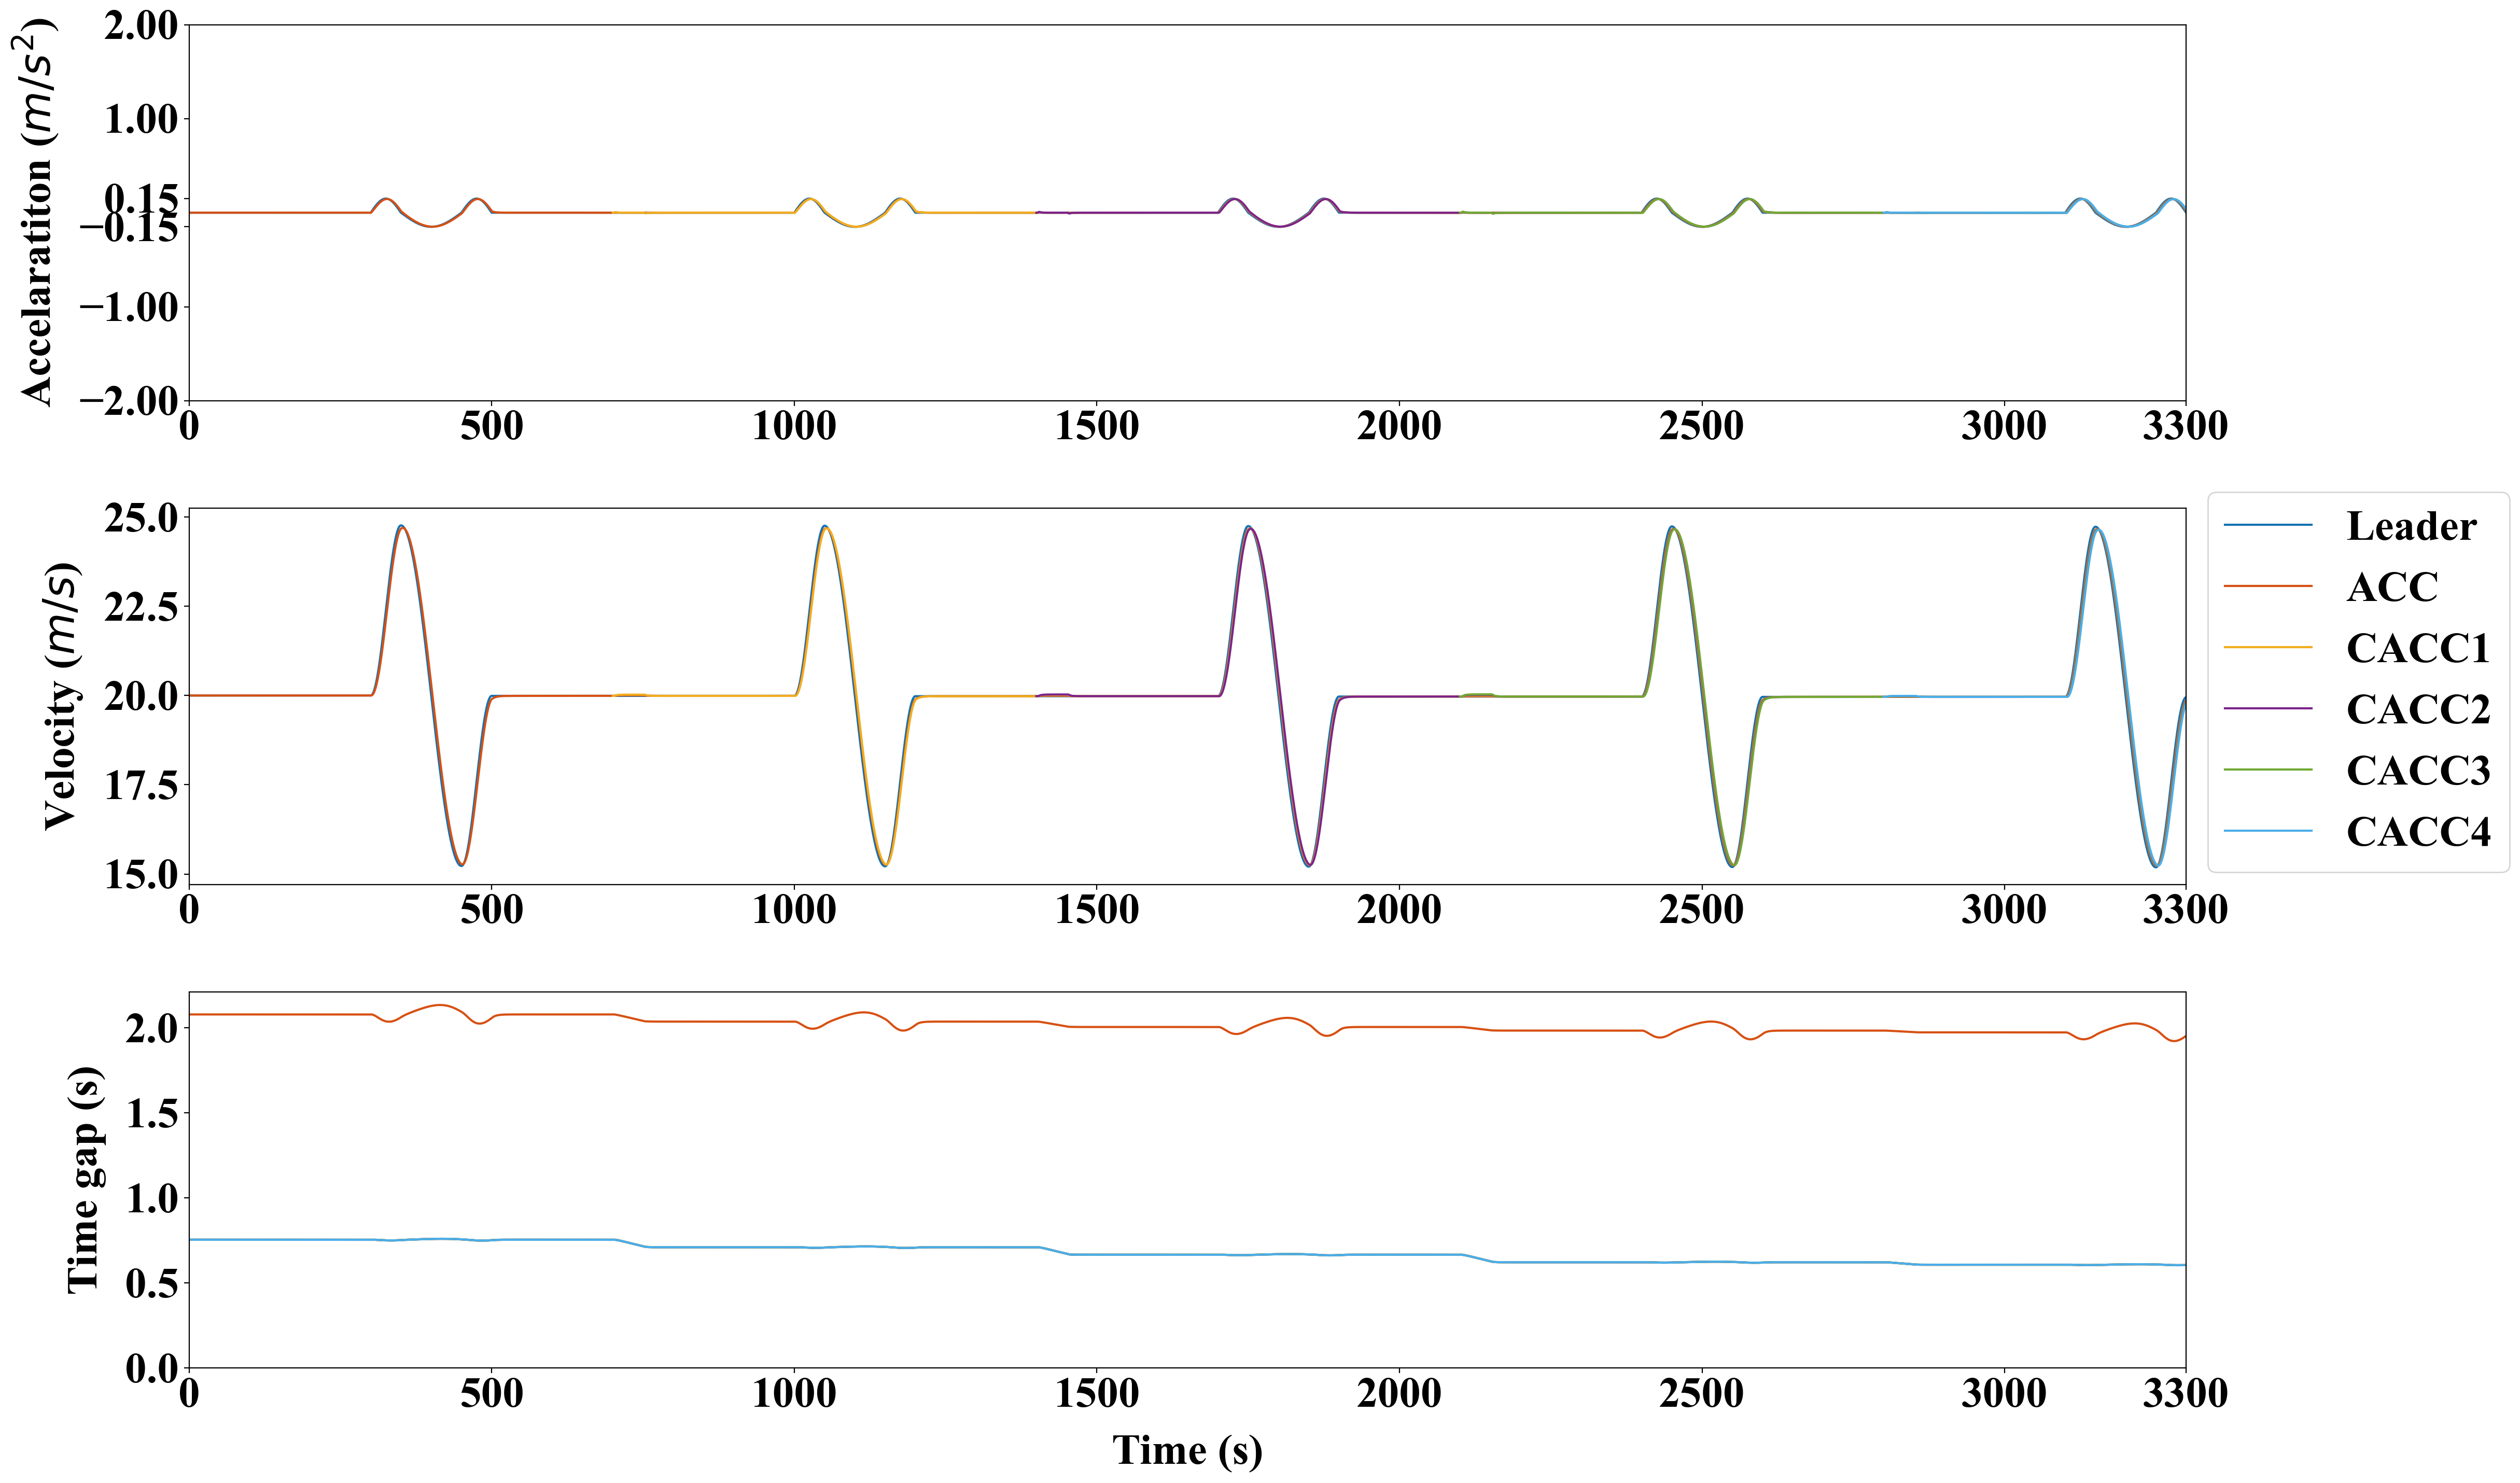
\includegraphics[width=14cm]{figs/fig11.png}
% 	\caption{Simulation results of experiment one: CACPC with YK parameterization under the platoon forming case.}
% 	\label{fig11}
% \end{figure}

% \begin{figure}
% 	\centering
% 		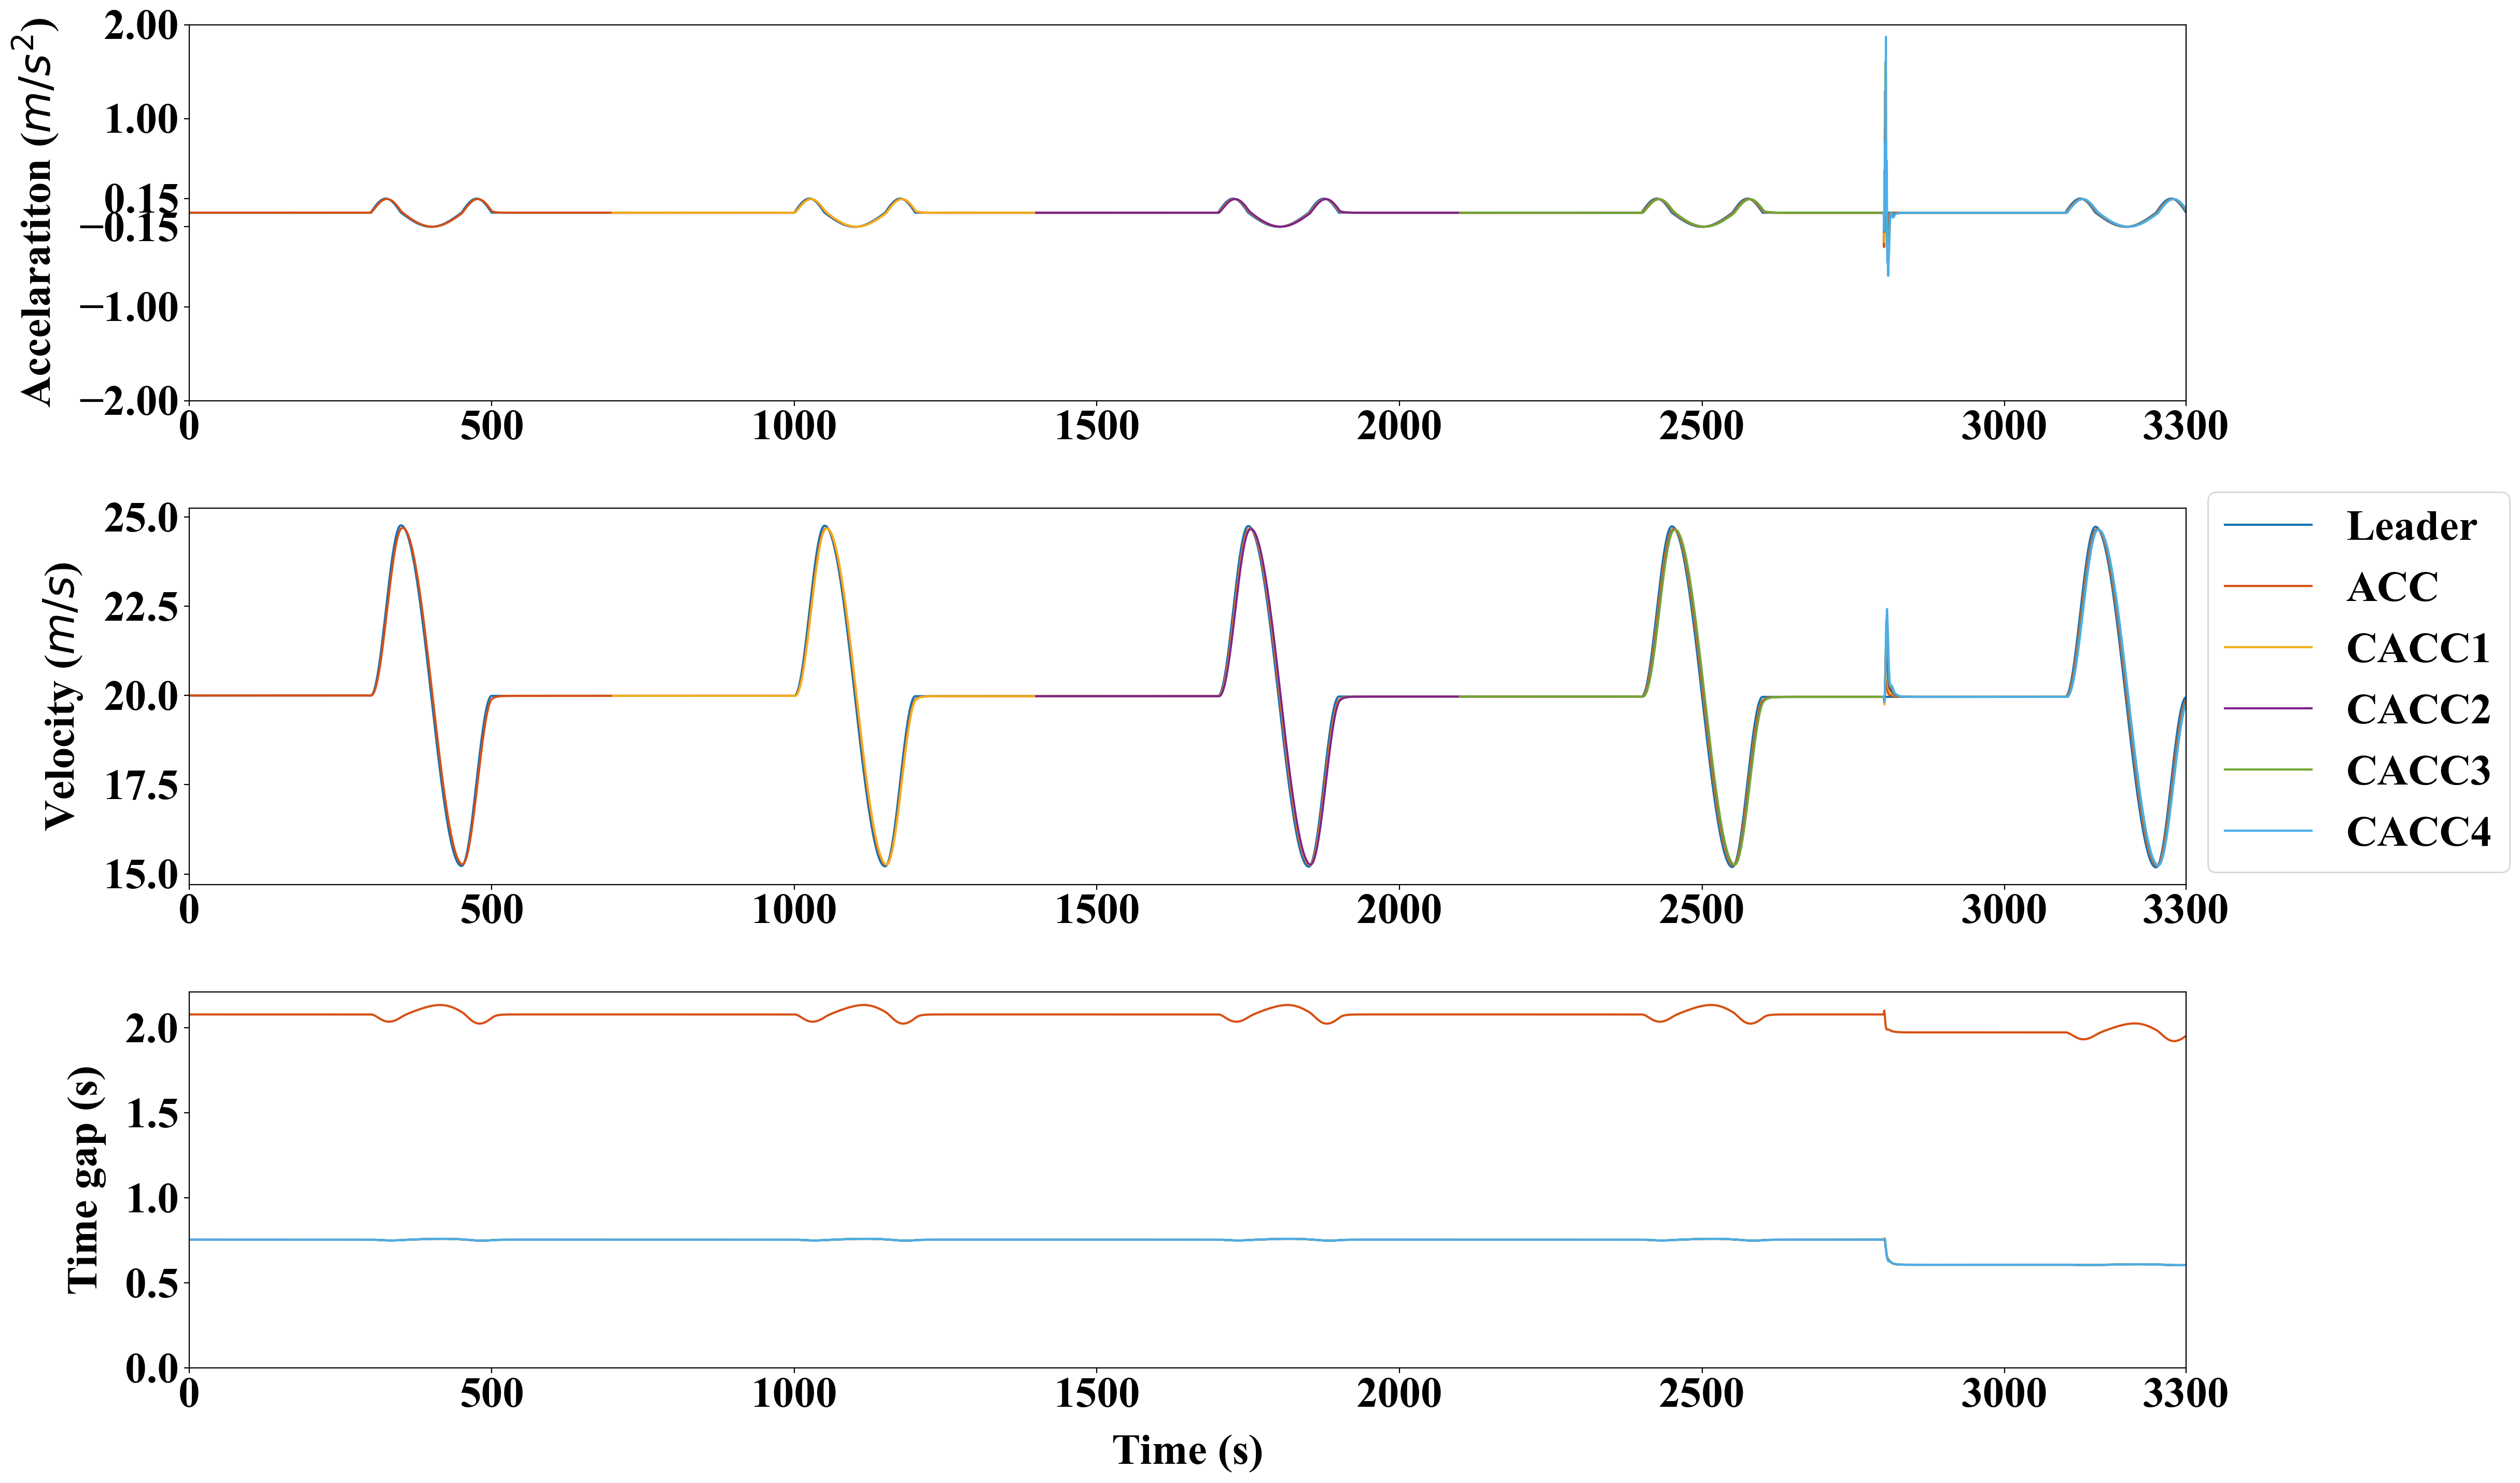
\includegraphics[width=14cm]{figs/fig12.png}
% 	\caption{Simulation results of experiment two: CACPC without YK parameterization under the platoon forming case.}
% 	\label{fig12}
% \end{figure}

% \begin{figure}
% 	\centering
% 		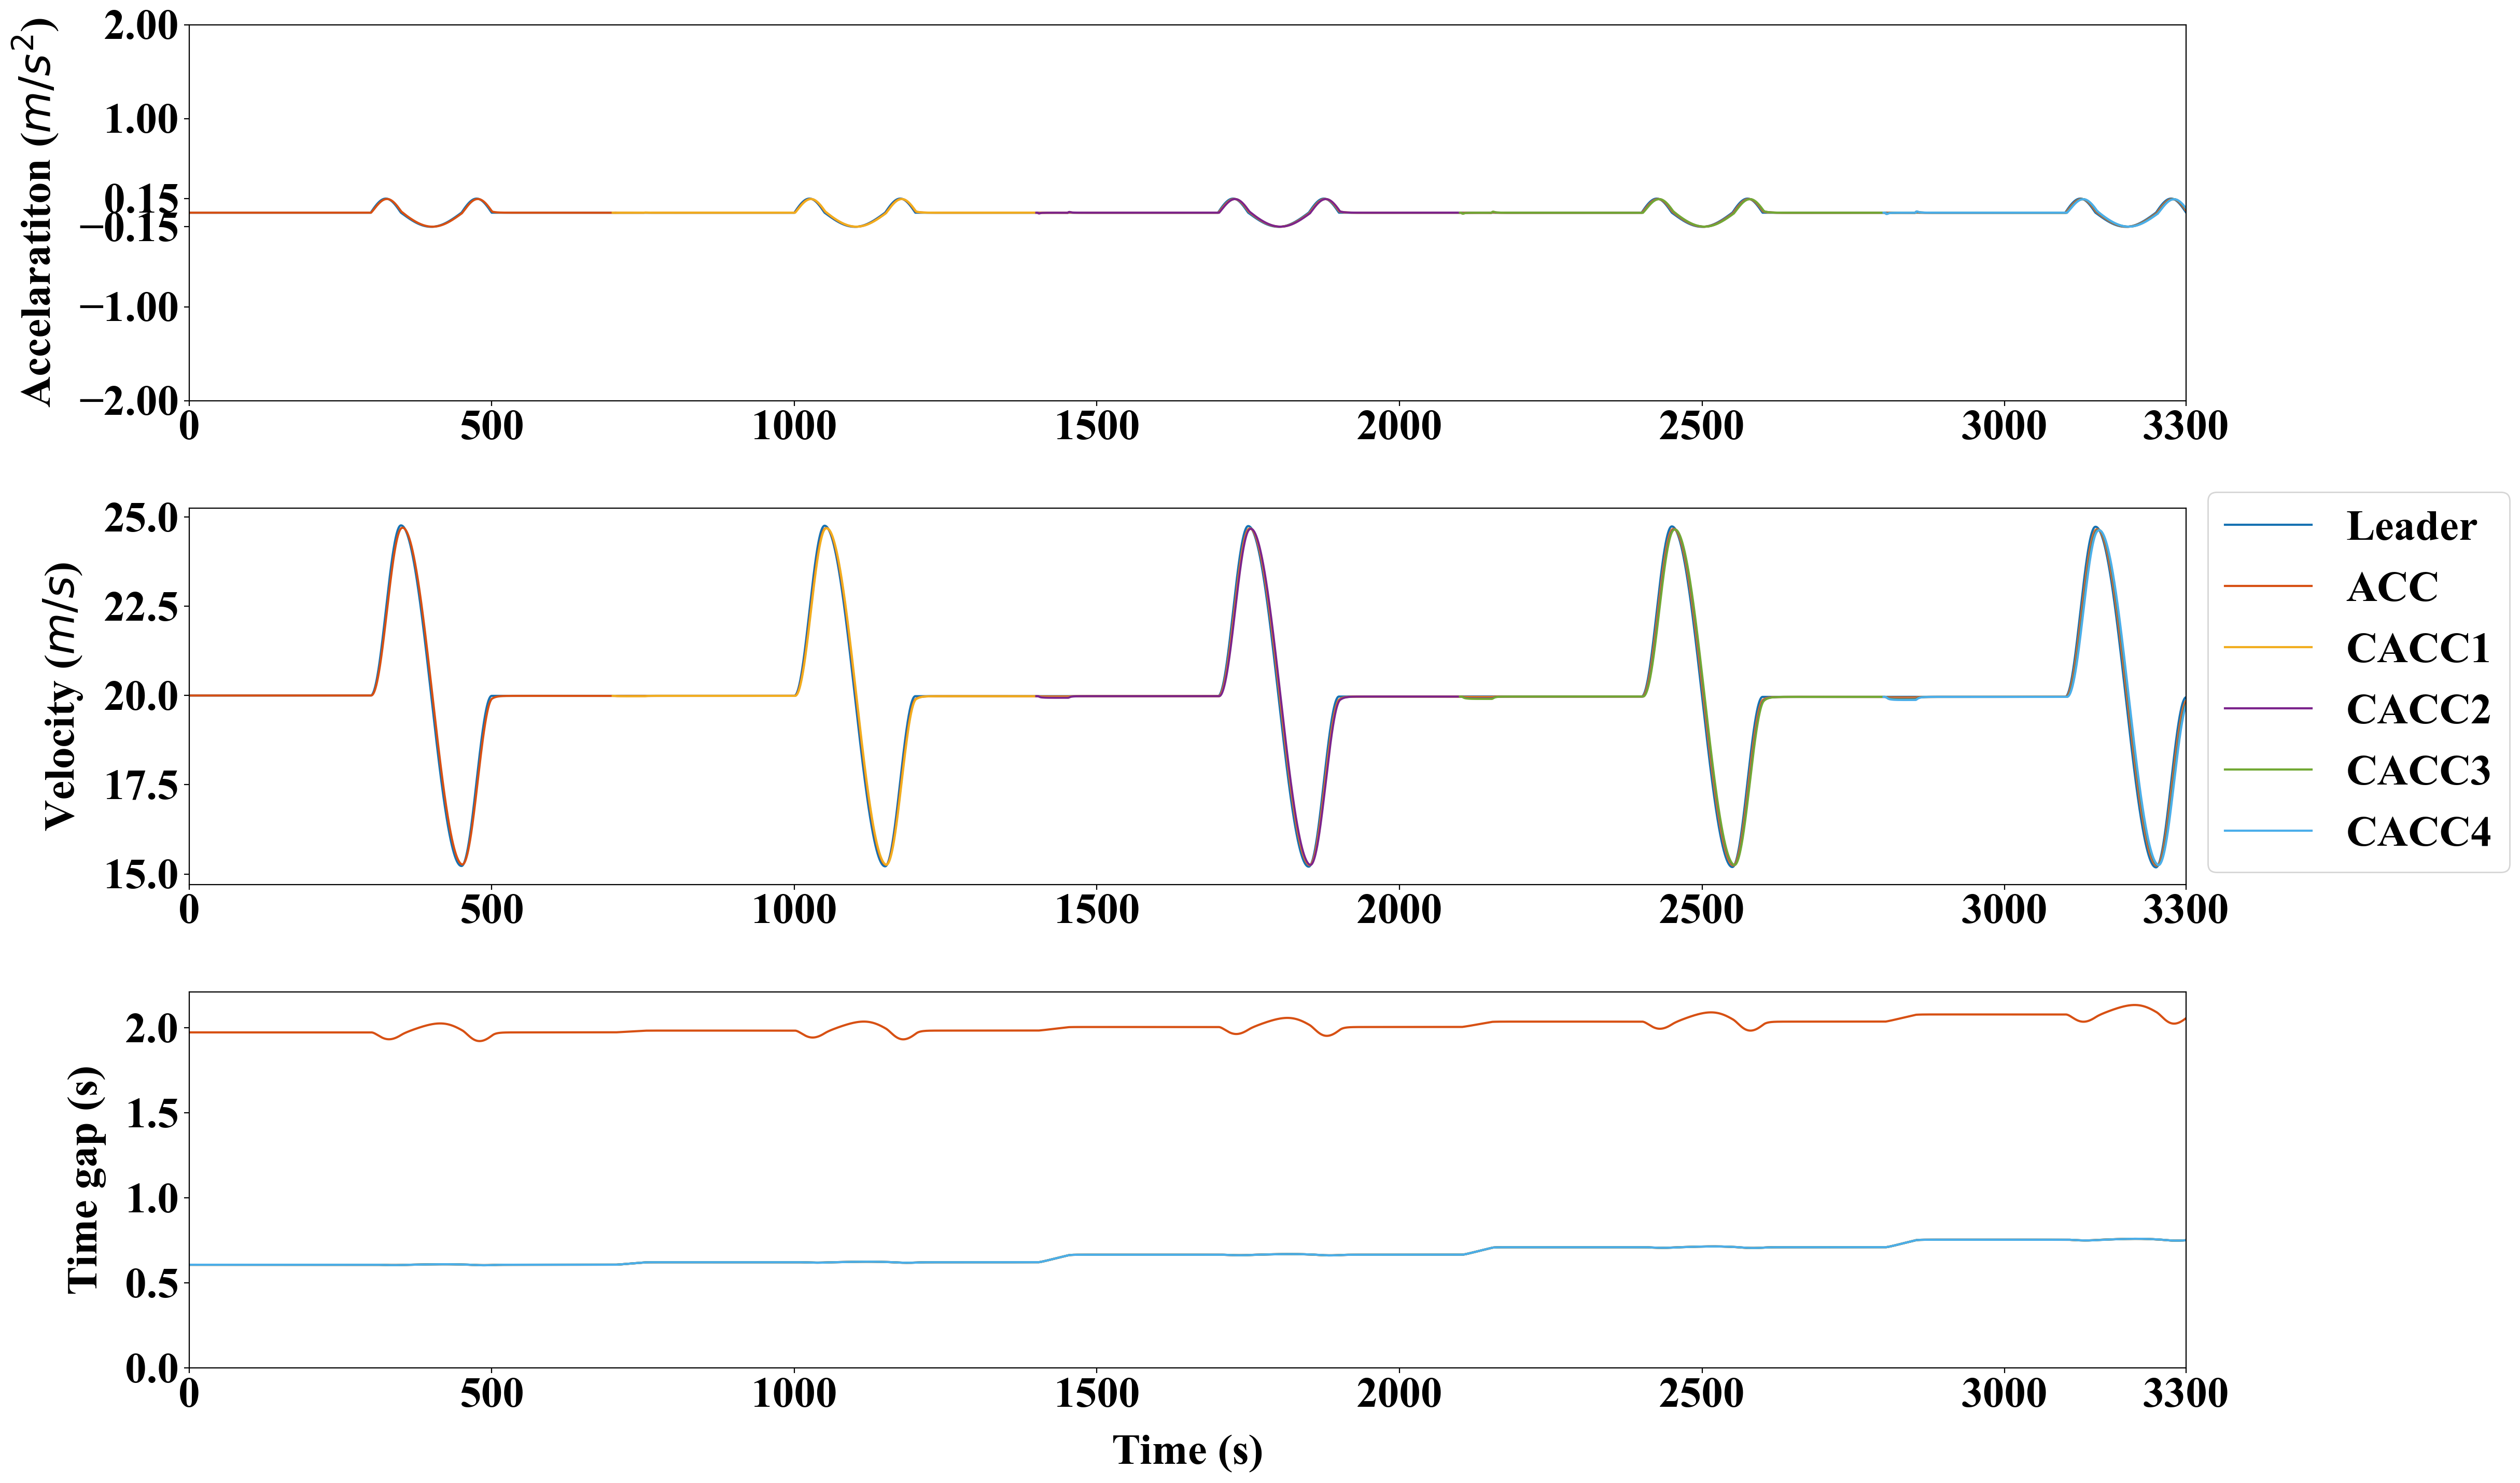
\includegraphics[width=14cm]{figs/extendfig1.png}
% 	\caption{Simulation results of experiment three: CACPC with YK parameterization under the platoon splitting case.}
% 	\label{extend1}
% \end{figure}

% \begin{figure}
% 	\centering
% 		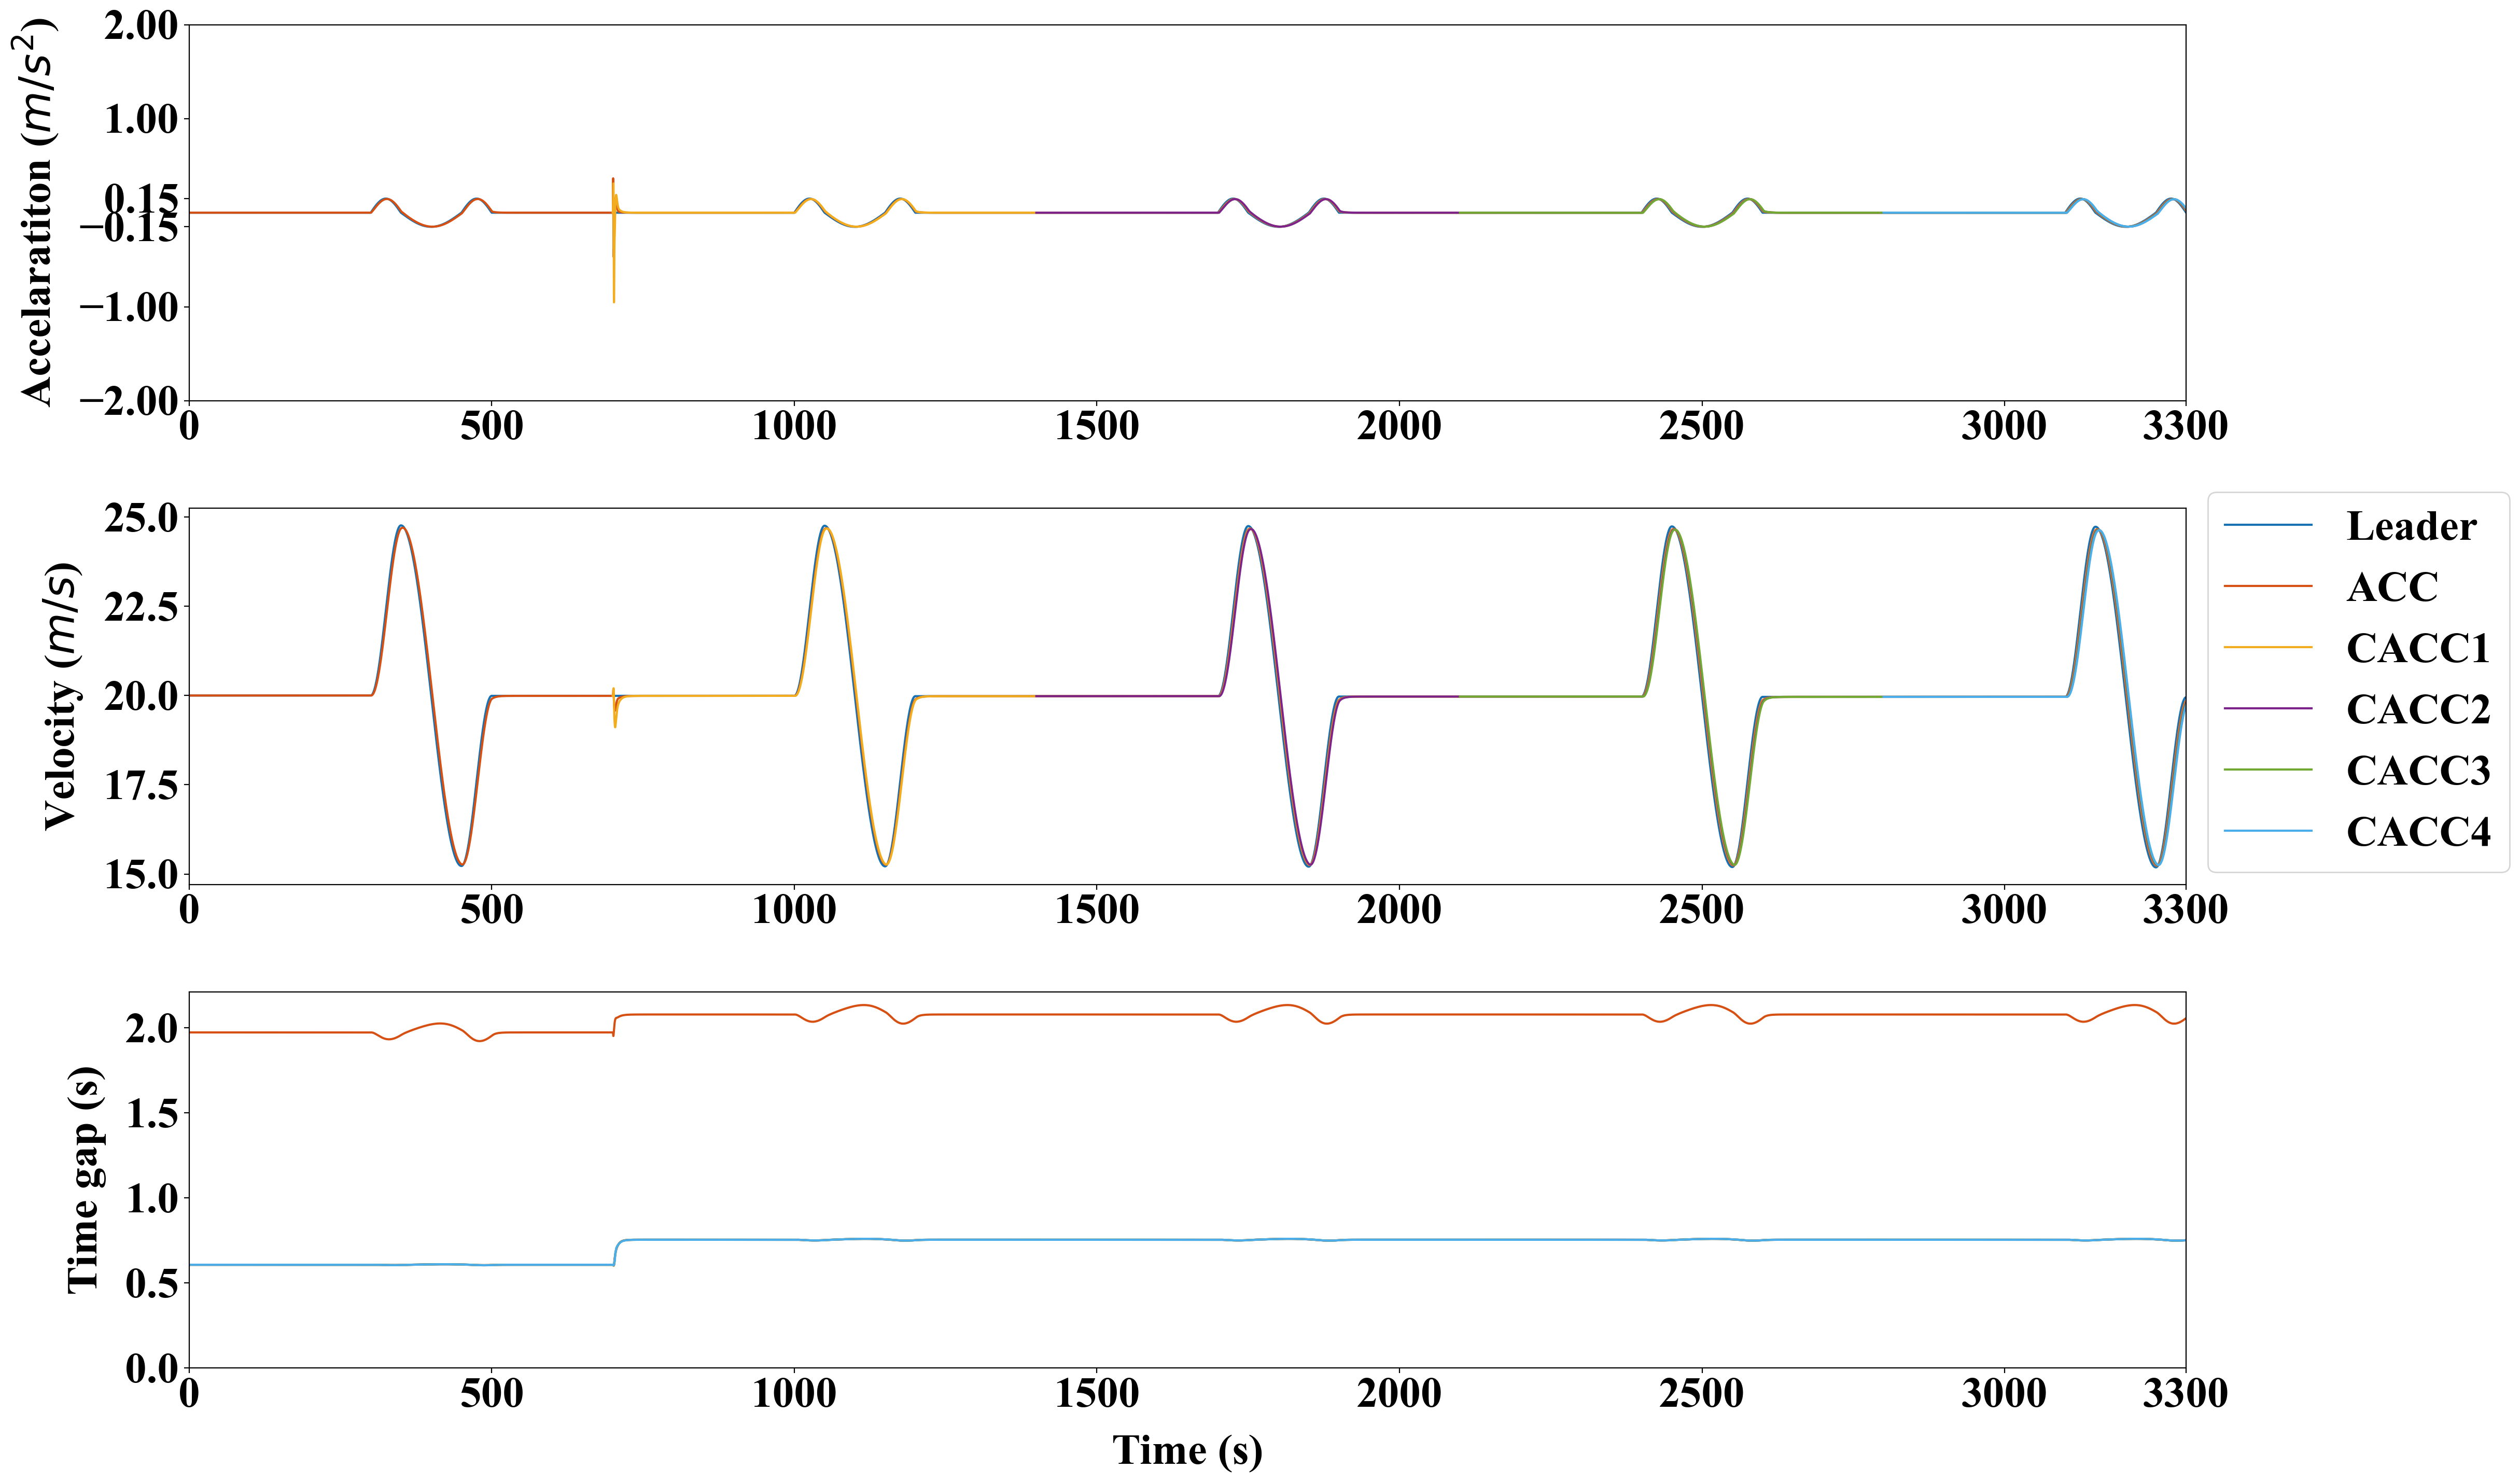
\includegraphics[width=14cm]{figs/extendfig2.png}
% 	\caption{Simulation results of experiment four: CACPC without YK parameterization under the platoon splitting case.}
% 	\label{extend2}
% \end{figure}

% \begin{figure}
% 	\centering
% 		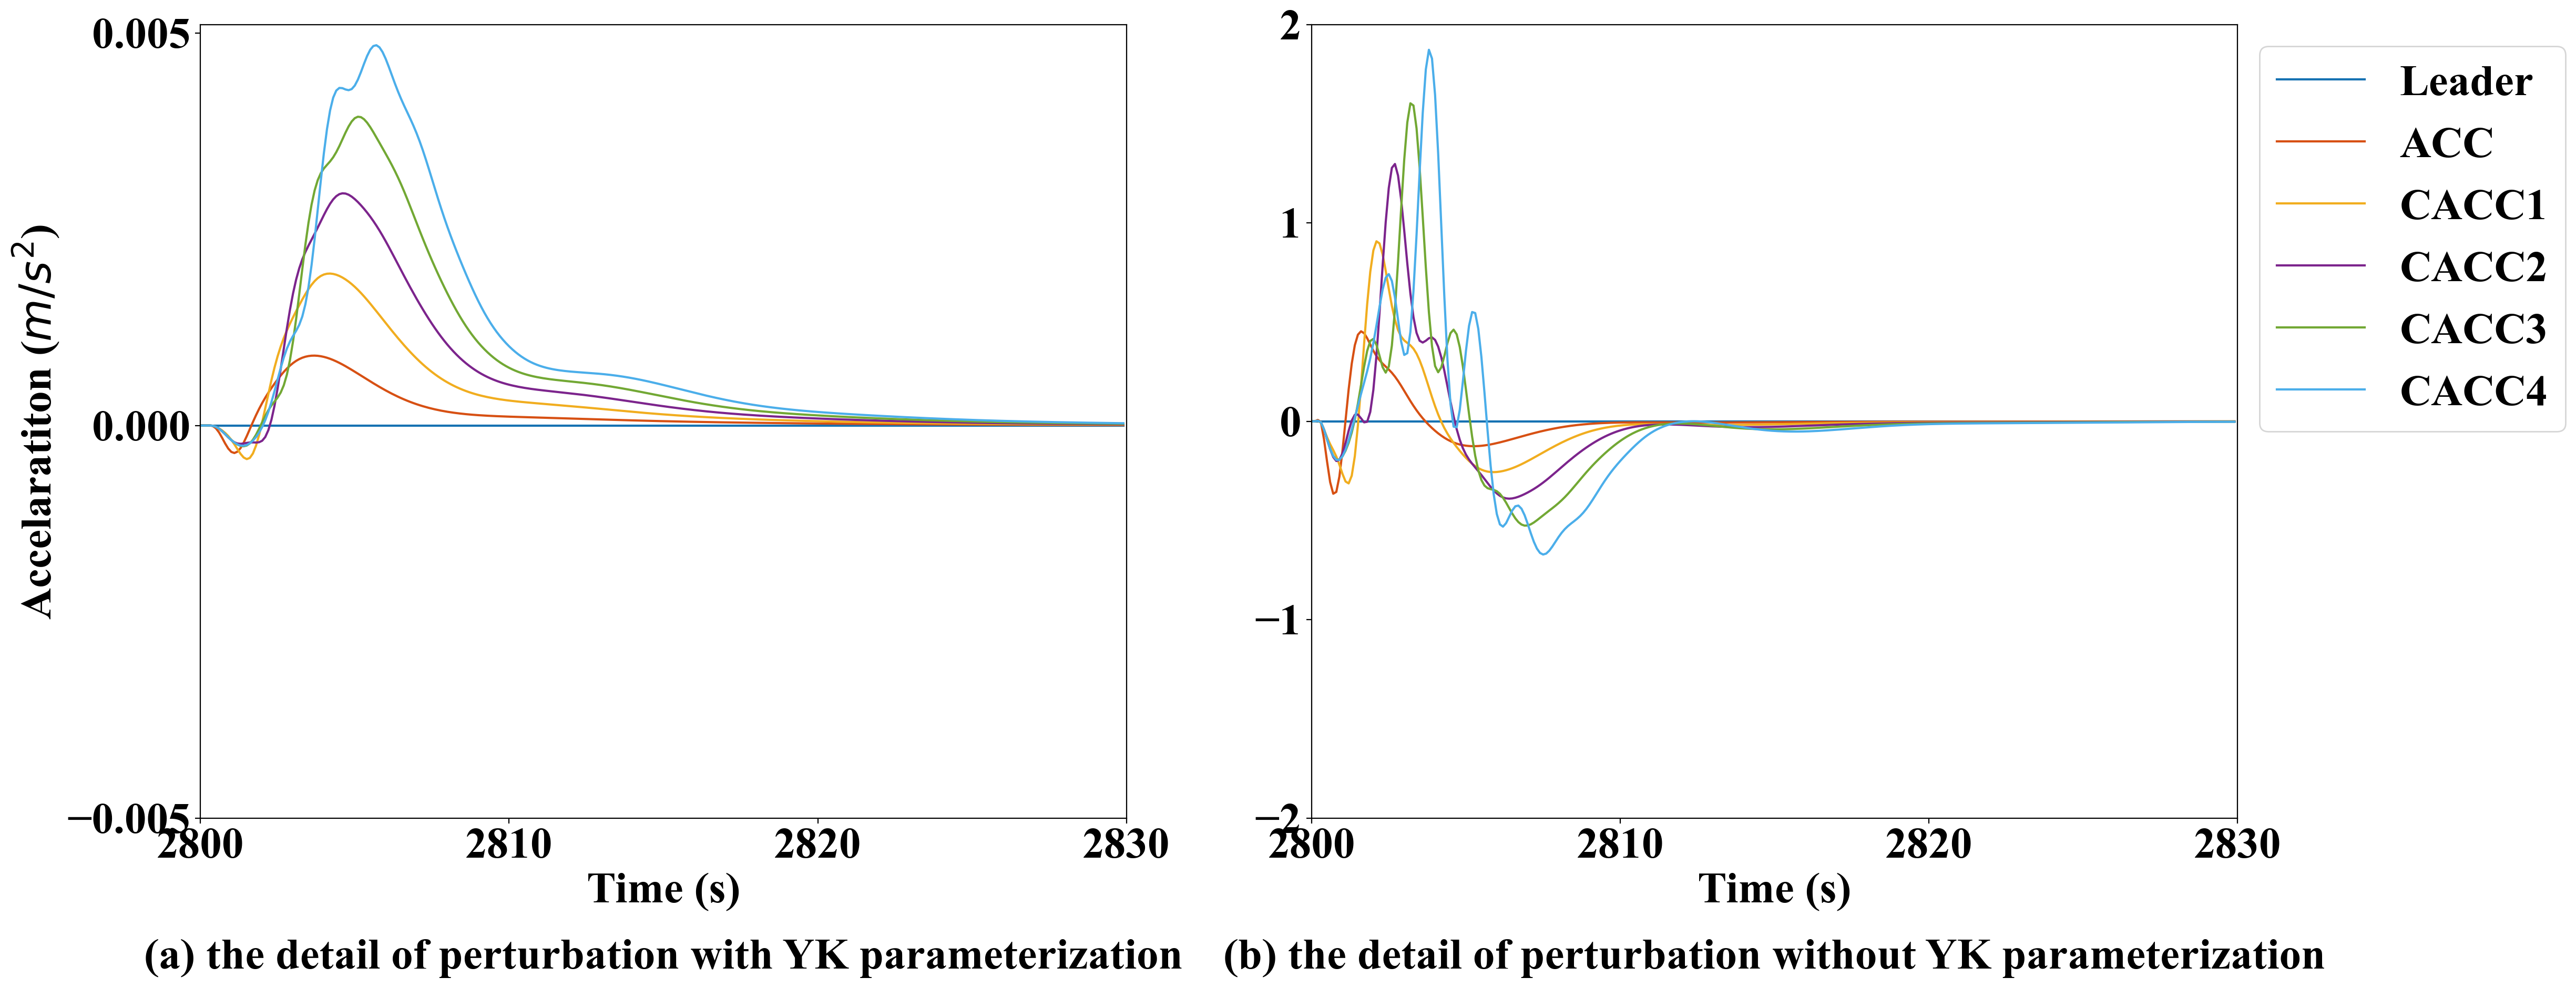
\includegraphics[width=14cm]{figs/extendfig5.png}
% 	\caption{Detailed perturbation simulation results of experiment one and two: CACPC with or without YK parameterization.}
% 	\label{extend5}
% \end{figure}


\textit{Simulation results}. Figure.~\ref{new1} and \ref{new3} show the results of experiments one,two, three and four, respectively. And figure.~\ref{new2} and \ref{new4} show the detailed perturbation simulation results of of experiments one,two, three and four. In figure.~\ref{new1} and \ref{new3}, (a)-(c) show the simulation results of the case with YK parameterization  and (d)-(f) show the simulation results of the case without YK parameterization where (a),(d) Acceleration of simulation results; (b),(e) Velocity of simulation results; (c),(f) Time gap of simulation results. As for figure.~\ref{new2} and \ref{new4}, (a)-(e) show the propagating processes of five applied perturbations and (f)-(i) show the four switching processes of the case with YK parameterization. And for the case without YK parameterization (j)-(n) show the propagating processes of five applied perturbations and (o)-(r) show the four switching processes.

In figure.~\ref{new1} and \ref{new2}, the process of the gradual formation of the CACC platoon with and without YK parameterization is clearly shown while the process of the gradual splitting is shown in figure.~\ref{new3} and \ref{new4}. The first attention is spontaneous perturbations during controller switching. From the comparison of figure.~\ref{new2} and \ref{new4}, we can find that the controller switching causes spontaneous perturbations in the process of platoon formation which caused by the changing of equivalent desired time gap. These spontaneous perturbations can be suppressed by applying the tuning function $\gamma$ to achieve smooth switching. However, in the case without YK parameterization, due to the direct switching when the platoon size reaches or leaves the trigger size, the spontaneous perturbation is too significant, which seriously impacts the stability and safety of the traffic flow. The second attention is string stability. All CACPCs applied under different CACC platoon sizes can maintain string stability through YK parameterization which is shown in figure.~\ref{new2} and \ref{new4}. Moreover, using YK parameterization can work under any CACC MPR since it can be applied even in a common scenario where the CACC MPR is low and the platoon size is small. But for the case without YK parameterization, the CACPCs do not function sufficiently until the set trigger platoon size is reached  which means the it is hard to function in a long period of time because there will be a long time until the CACC MPR gets high. In addition, because the splitting process and forming process is similar, the following simulation experiments are only conducted in the forming process. Notice that from the difference on the acceleration between subplot (a) and (b) in figure.~\ref{new1} and \ref{new3} which is detailed shown in subplot (k-r) in figure.~\ref{new2} and \ref{new4}, and a misunderstood conclusion can be drawn because the perturbation is amplified with or without YK parameterization. However, the perturbation is caused by the increasing of the equivalent desired time gap during the controller switching. In the case with YK parameterization, the perturbation only raise once then back to the equivalent state. And for the case without YK parameterization, the perturbation is fluctuating during the propagating process which means the switching progress is not smooth enough to make the perturbation supperssed.

\subsubsection{Simulation experiments maintain a fluctuating speed during the forming process}
\label{Section 5.2.2}

\textit{Simulation scenario:} The simulation scenario is similiar to the experiment one in Section. ~\ref{Section 5.2.1}, but different in the given speed and acceleration configuration of the leader vehicle. In this simulation experiment, the speed of leader vehicle is fluctuating all the time to simulate the traffic oscillation scenario. There are two experiments conducted:
\begin{enumerate}
  \item \textit{Experiment five:} The forming process of the CACC platoon with YK parameterization under the fluctuating velocity case where an ACC (which is a CACC but degraded to an ACC functionally) follows the leader at the beginning, and more CACCs join the CACC platoon one by one at the simulation time of 700s, 1400s, 2100s, and 2800s.
  \item \textit{Experiment six:} The forming process of the CACC platoon without YK parameterization under the fluctuating velocity case where an ACC (which is a CACC but degraded to an ACC functionally) follows the leader at the beginning, and more CACCs join the CACC platoon one by one at the simulation time of 700s, 1400s, 2100s, and 2800s.
\end{enumerate}

\begin{figure}
  \centering
  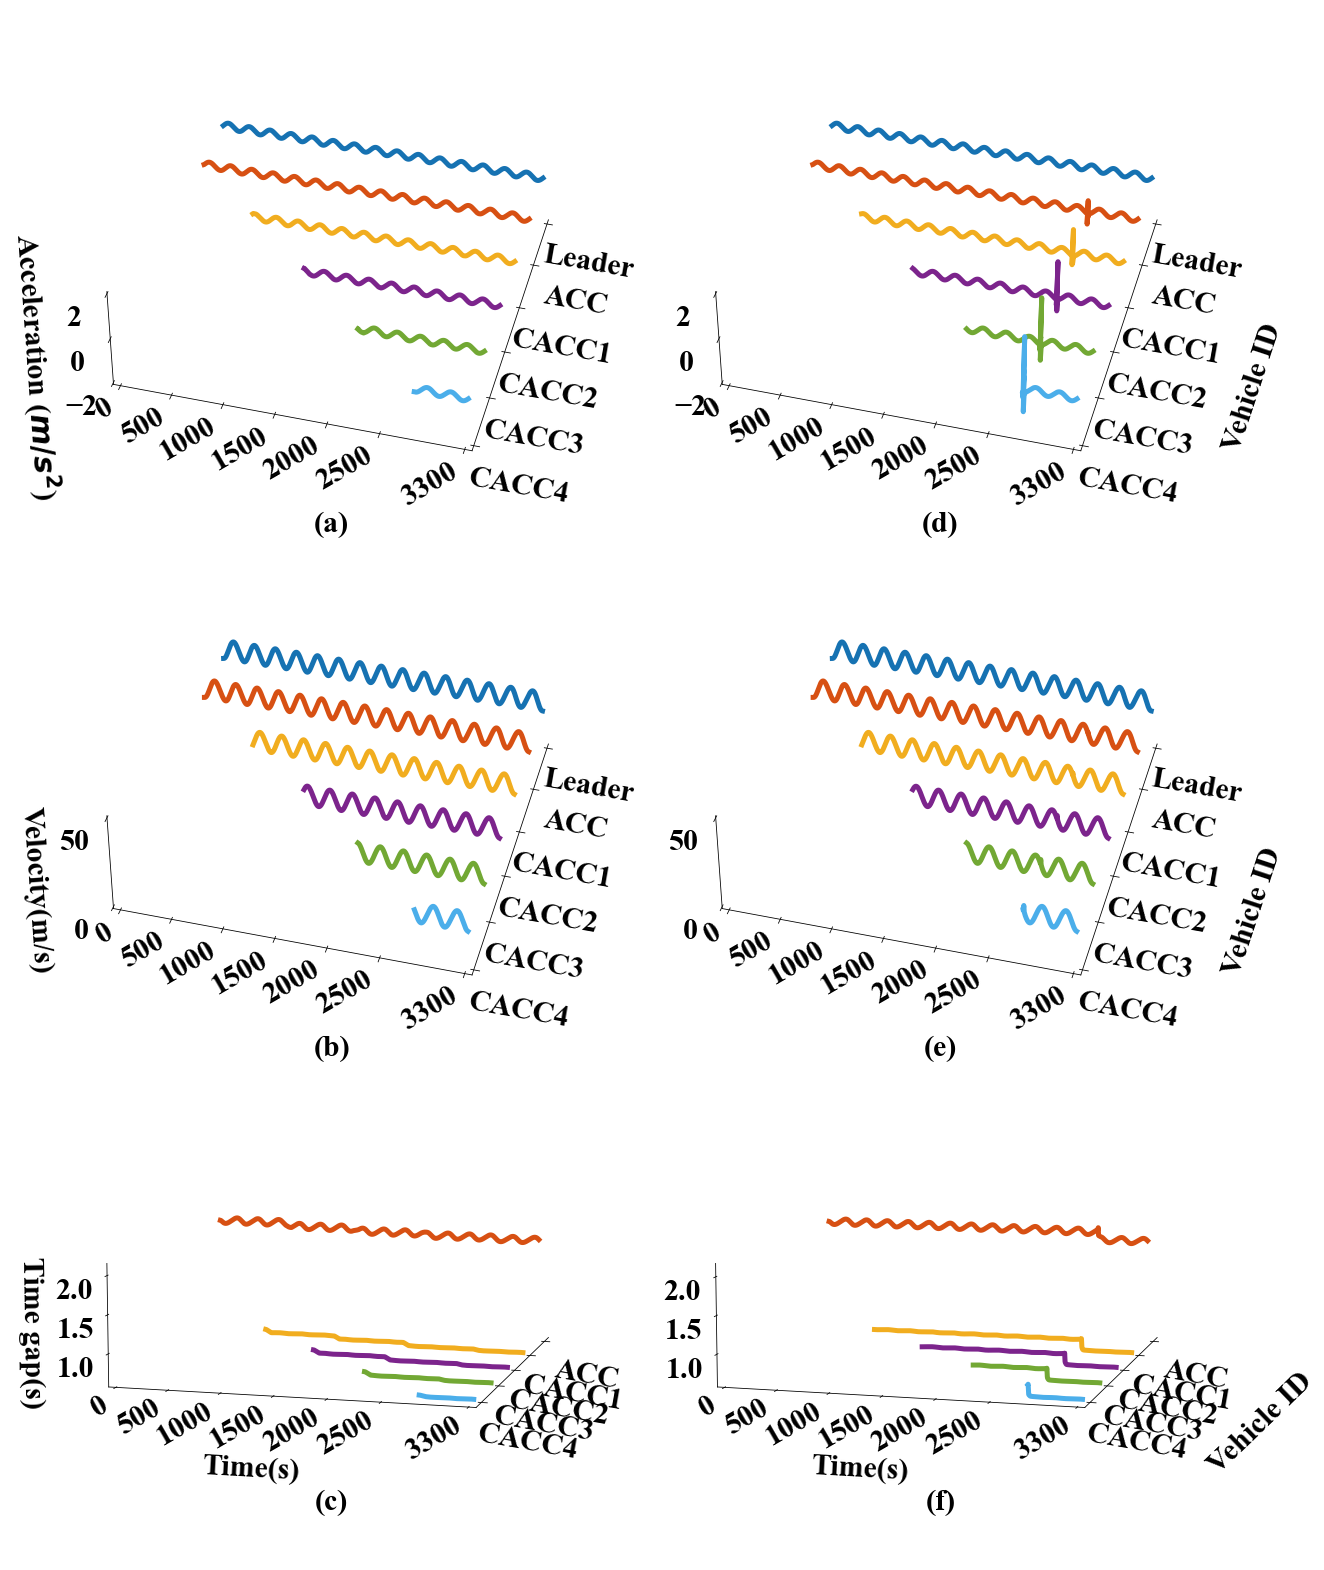
\includegraphics[width=14cm]{figs/f_YK_form.png}
  \caption{~Simulation results of experiment five and six: CACPC with or without YK parameterization under the fluctuating velocity case. (a)-(c) show the simulation results of experiment five and (d)-(f) show the simulation results of experiment six. (a),(d) Acceleration of simulation results; (b),(e) Velocity of simulation results; (c),(f) Time gap of simulation results.}
  \label{new5}
\end{figure}

\begin{figure}
  \centering
  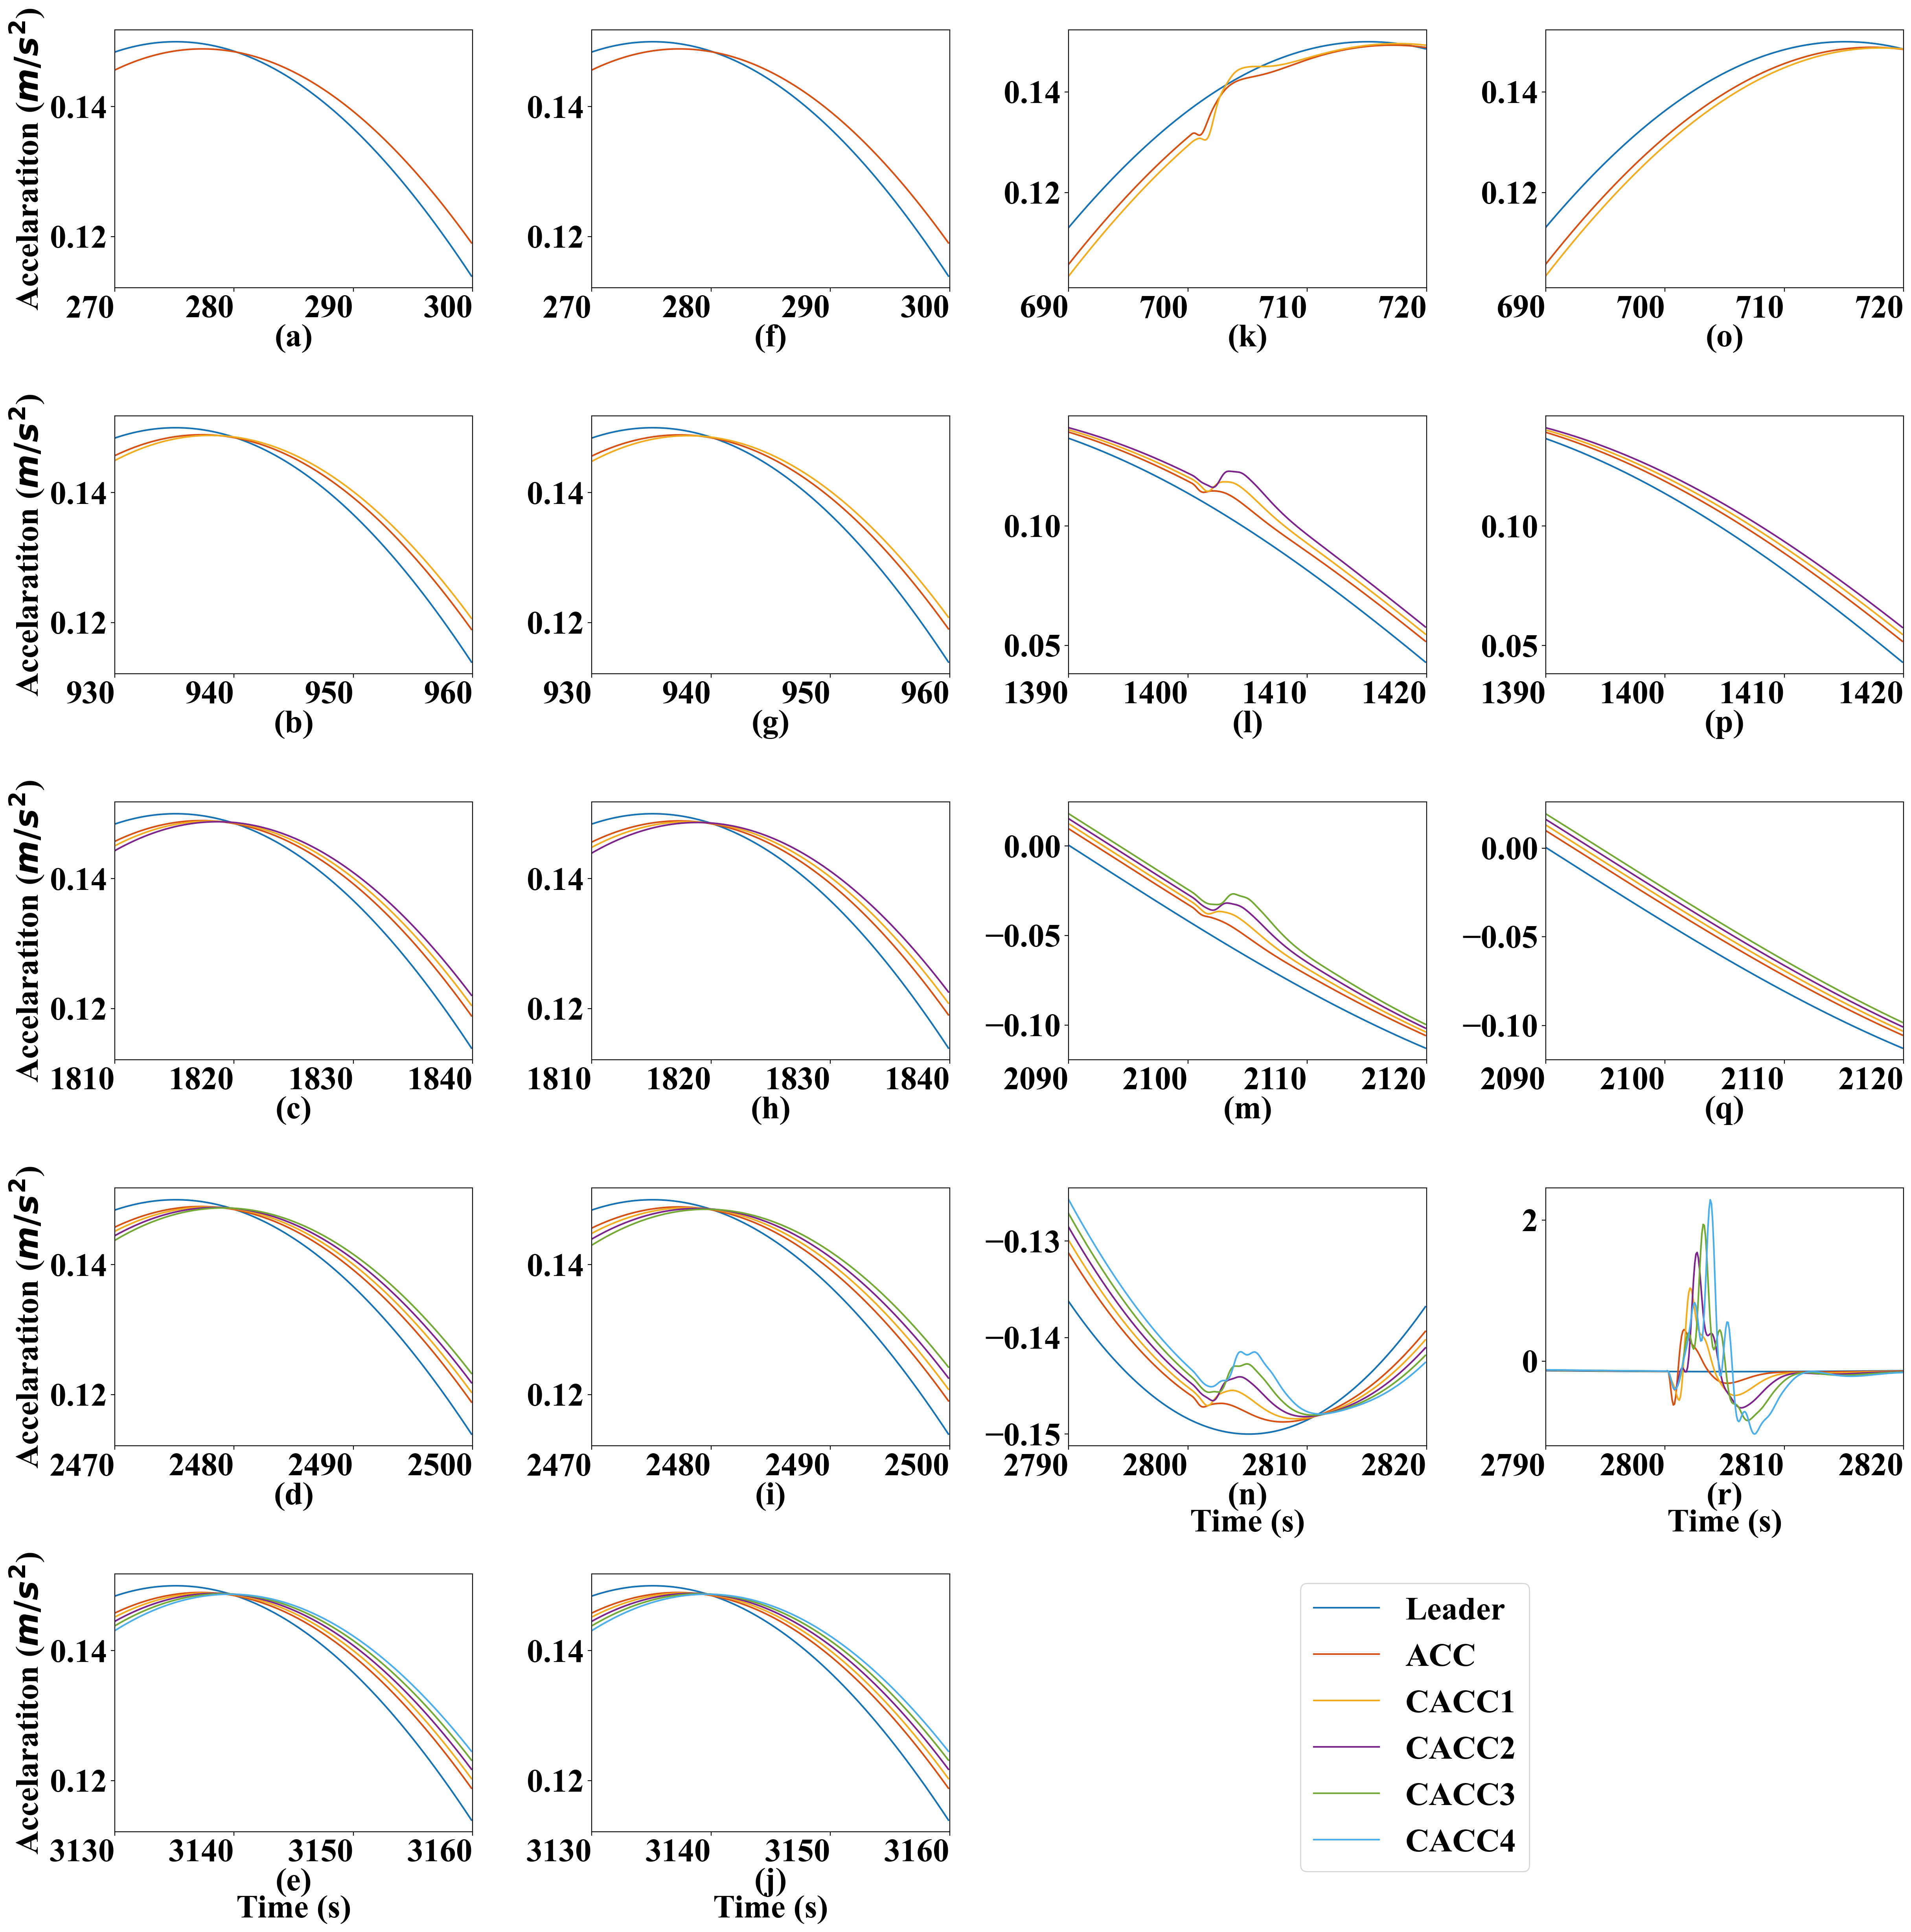
\includegraphics[width=14cm]{figs/fluat_detail.png}
  \caption{~Detailed perturbation simulation results of experiment five and six: CACPC with or without YK parameterization under the fluctuating velocity case. For experiment five, (a)-(e) show the propagating processes of five applied perturbations and (k)-(l) show the four switching processes. For experiment six, (f)-(j) show the propagating processes of five applied perturbations and (o)-(r) show the four switching processes.}
  \label{new6}
\end{figure}

% \begin{figure}
% 	\centering
% 		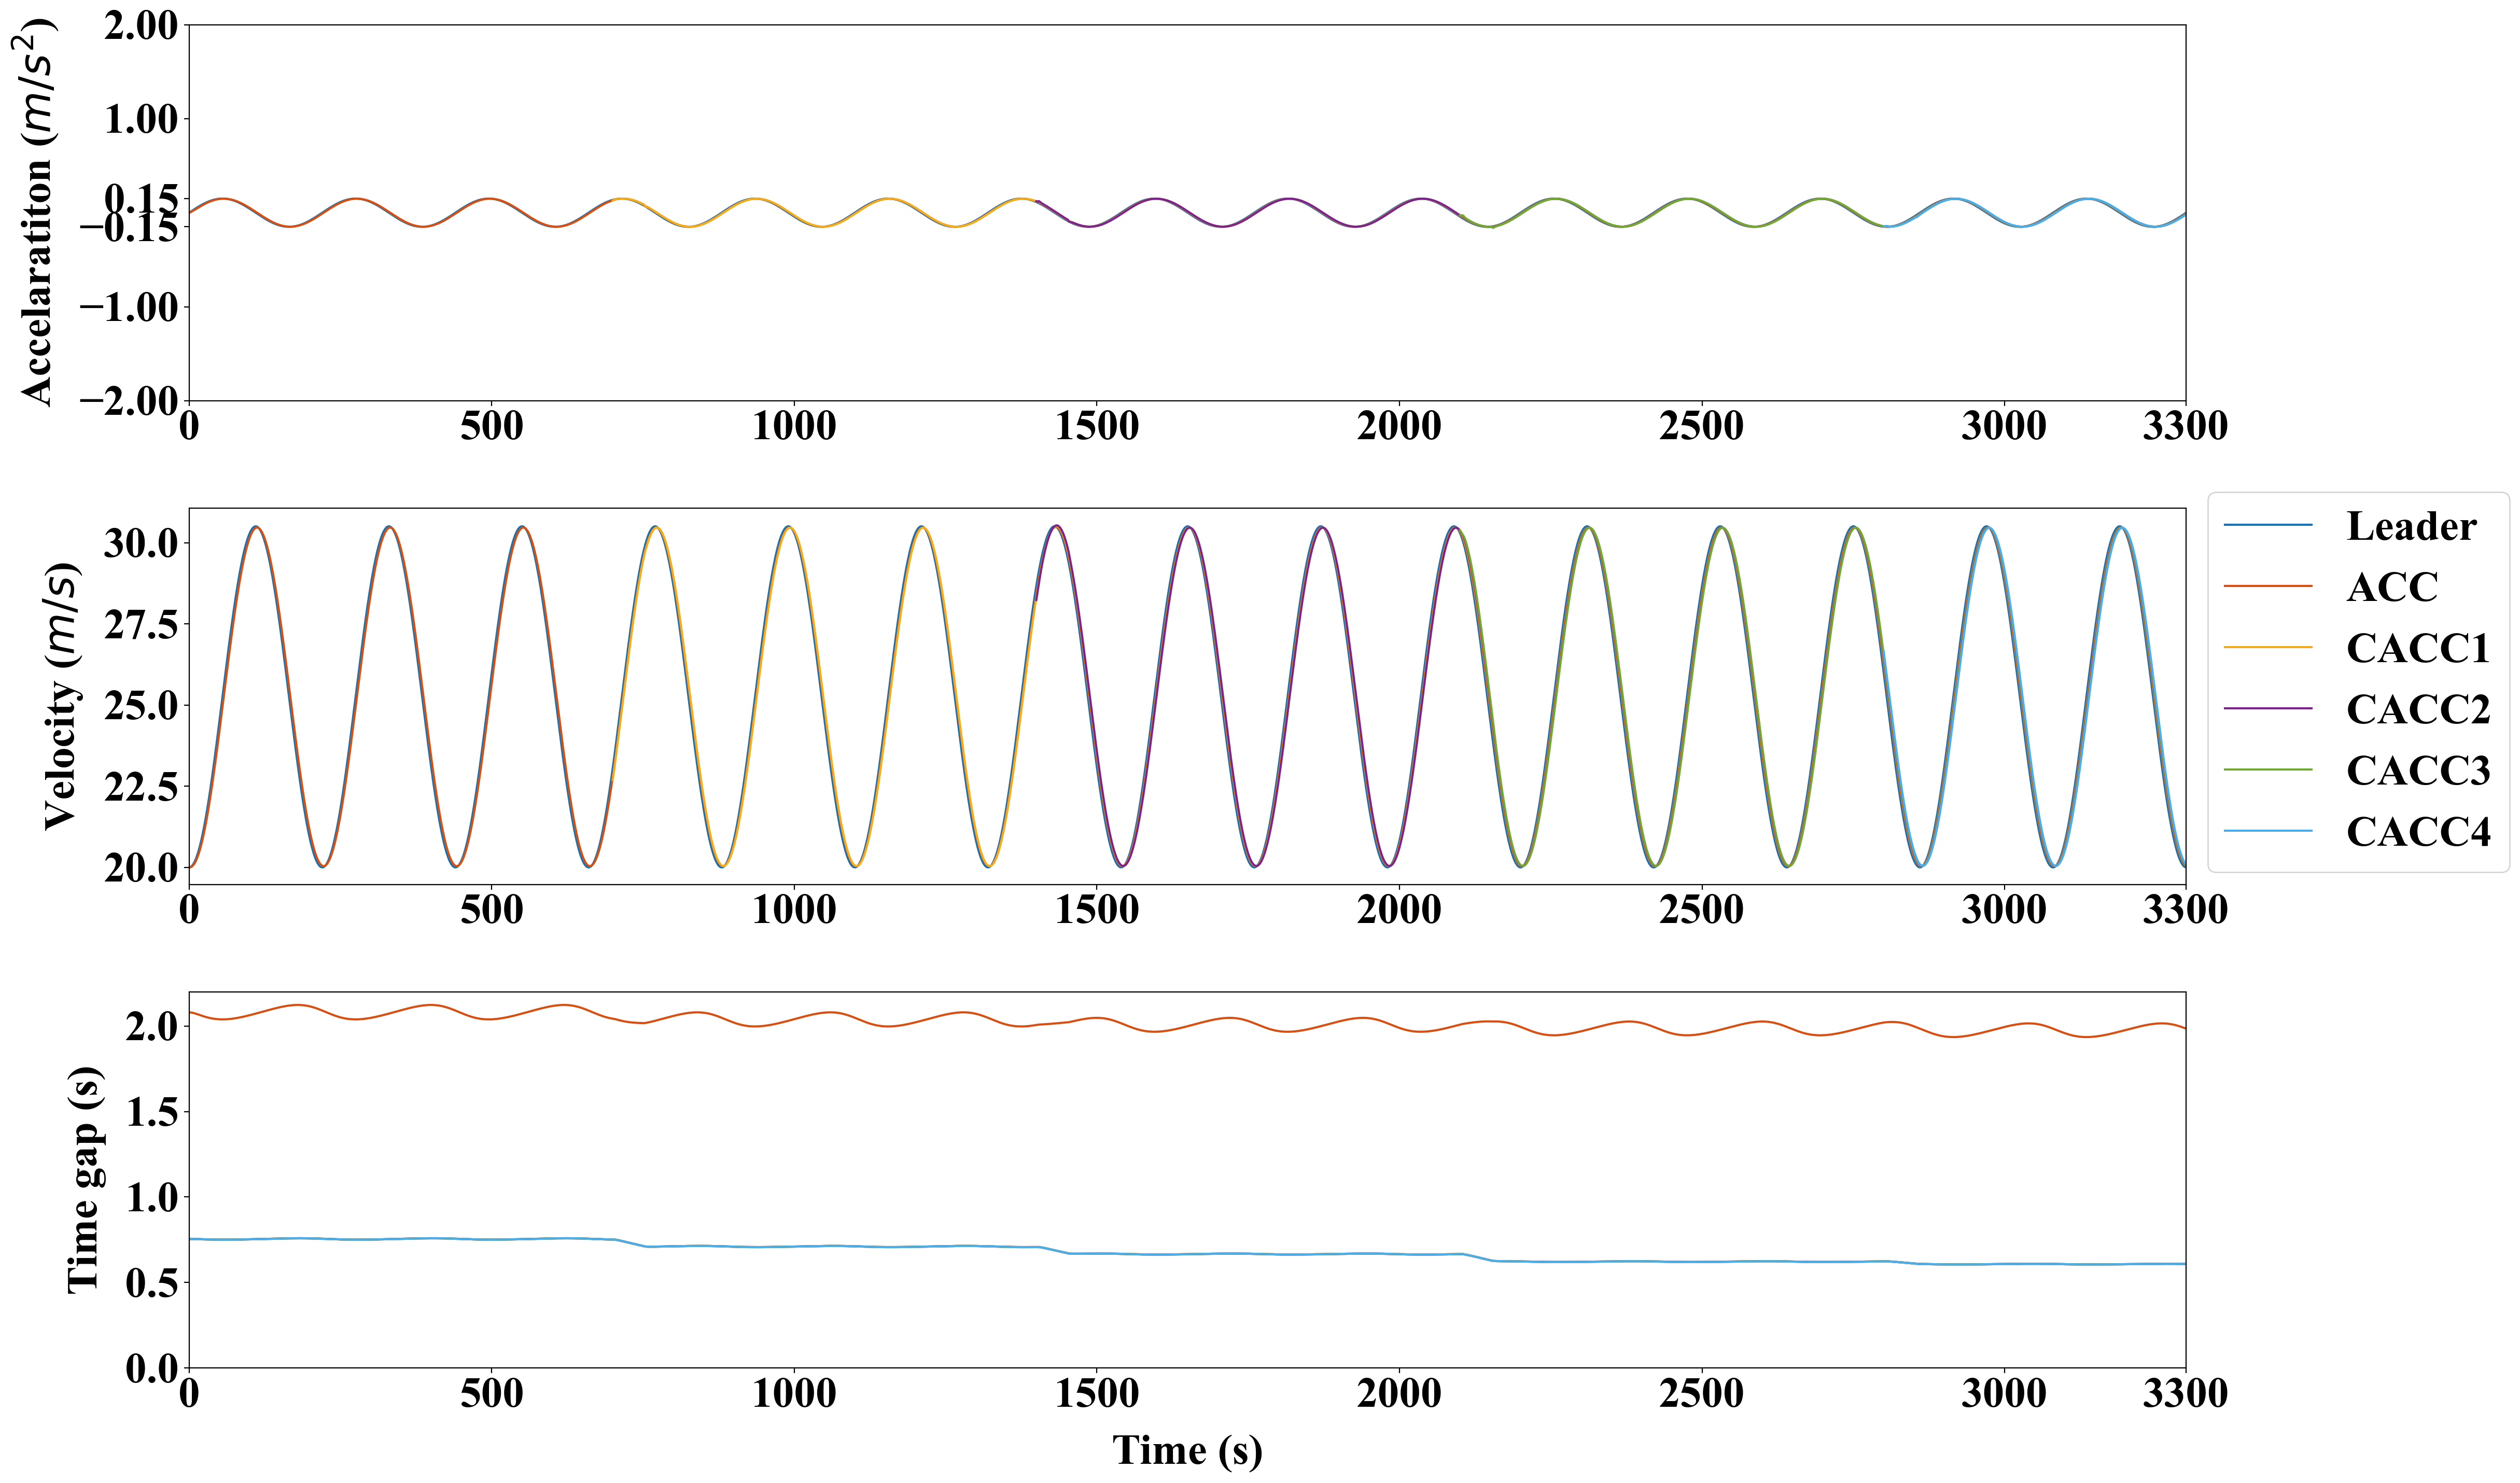
\includegraphics[width=14cm]{figs/extendfig3.png}
% 	\caption{~Simulation results of experiment five: CACPC with YK parameterization under the platoon forming case.}
% 	\label{extend3}
% \end{figure}

% \begin{figure}
% 	\centering
% 		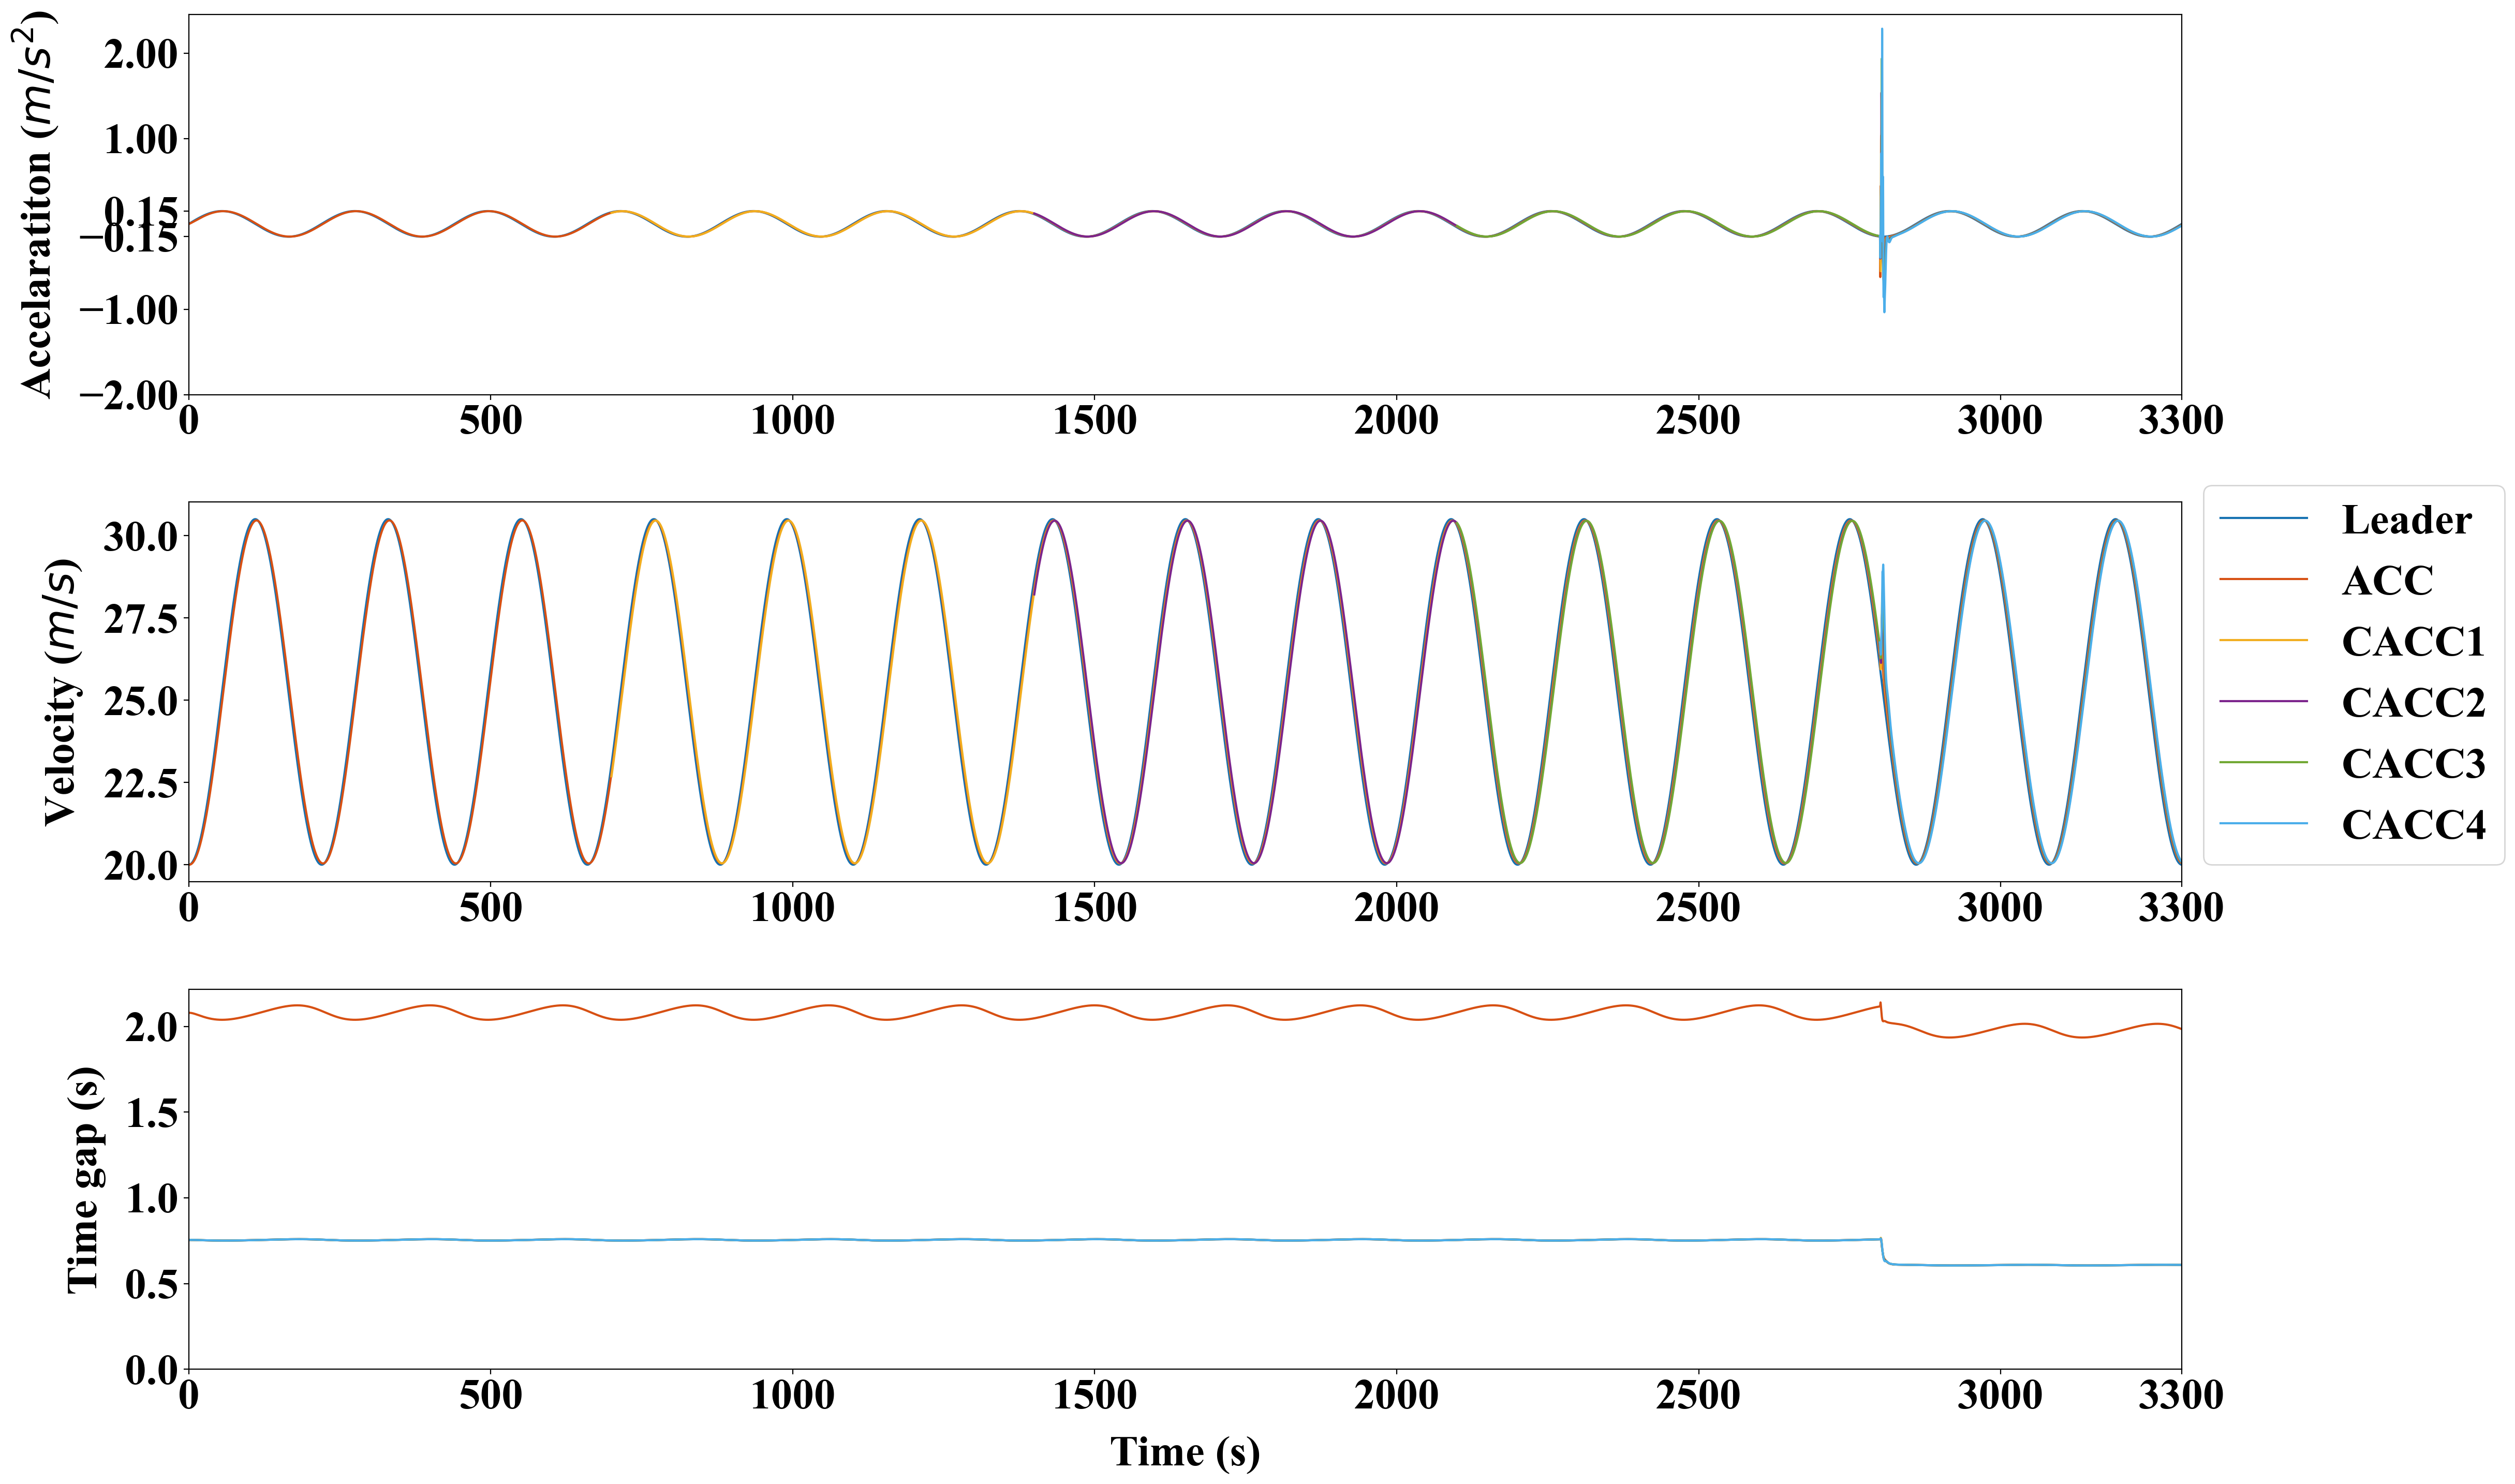
\includegraphics[width=14cm]{figs/extendfig4.png}
% 	\caption{~Simulation results of experiment six: CACPC without YK parameterization under the platoon forming case.}
% 	\label{extend4}
% \end{figure}

% \begin{figure}
% 	\centering
% 		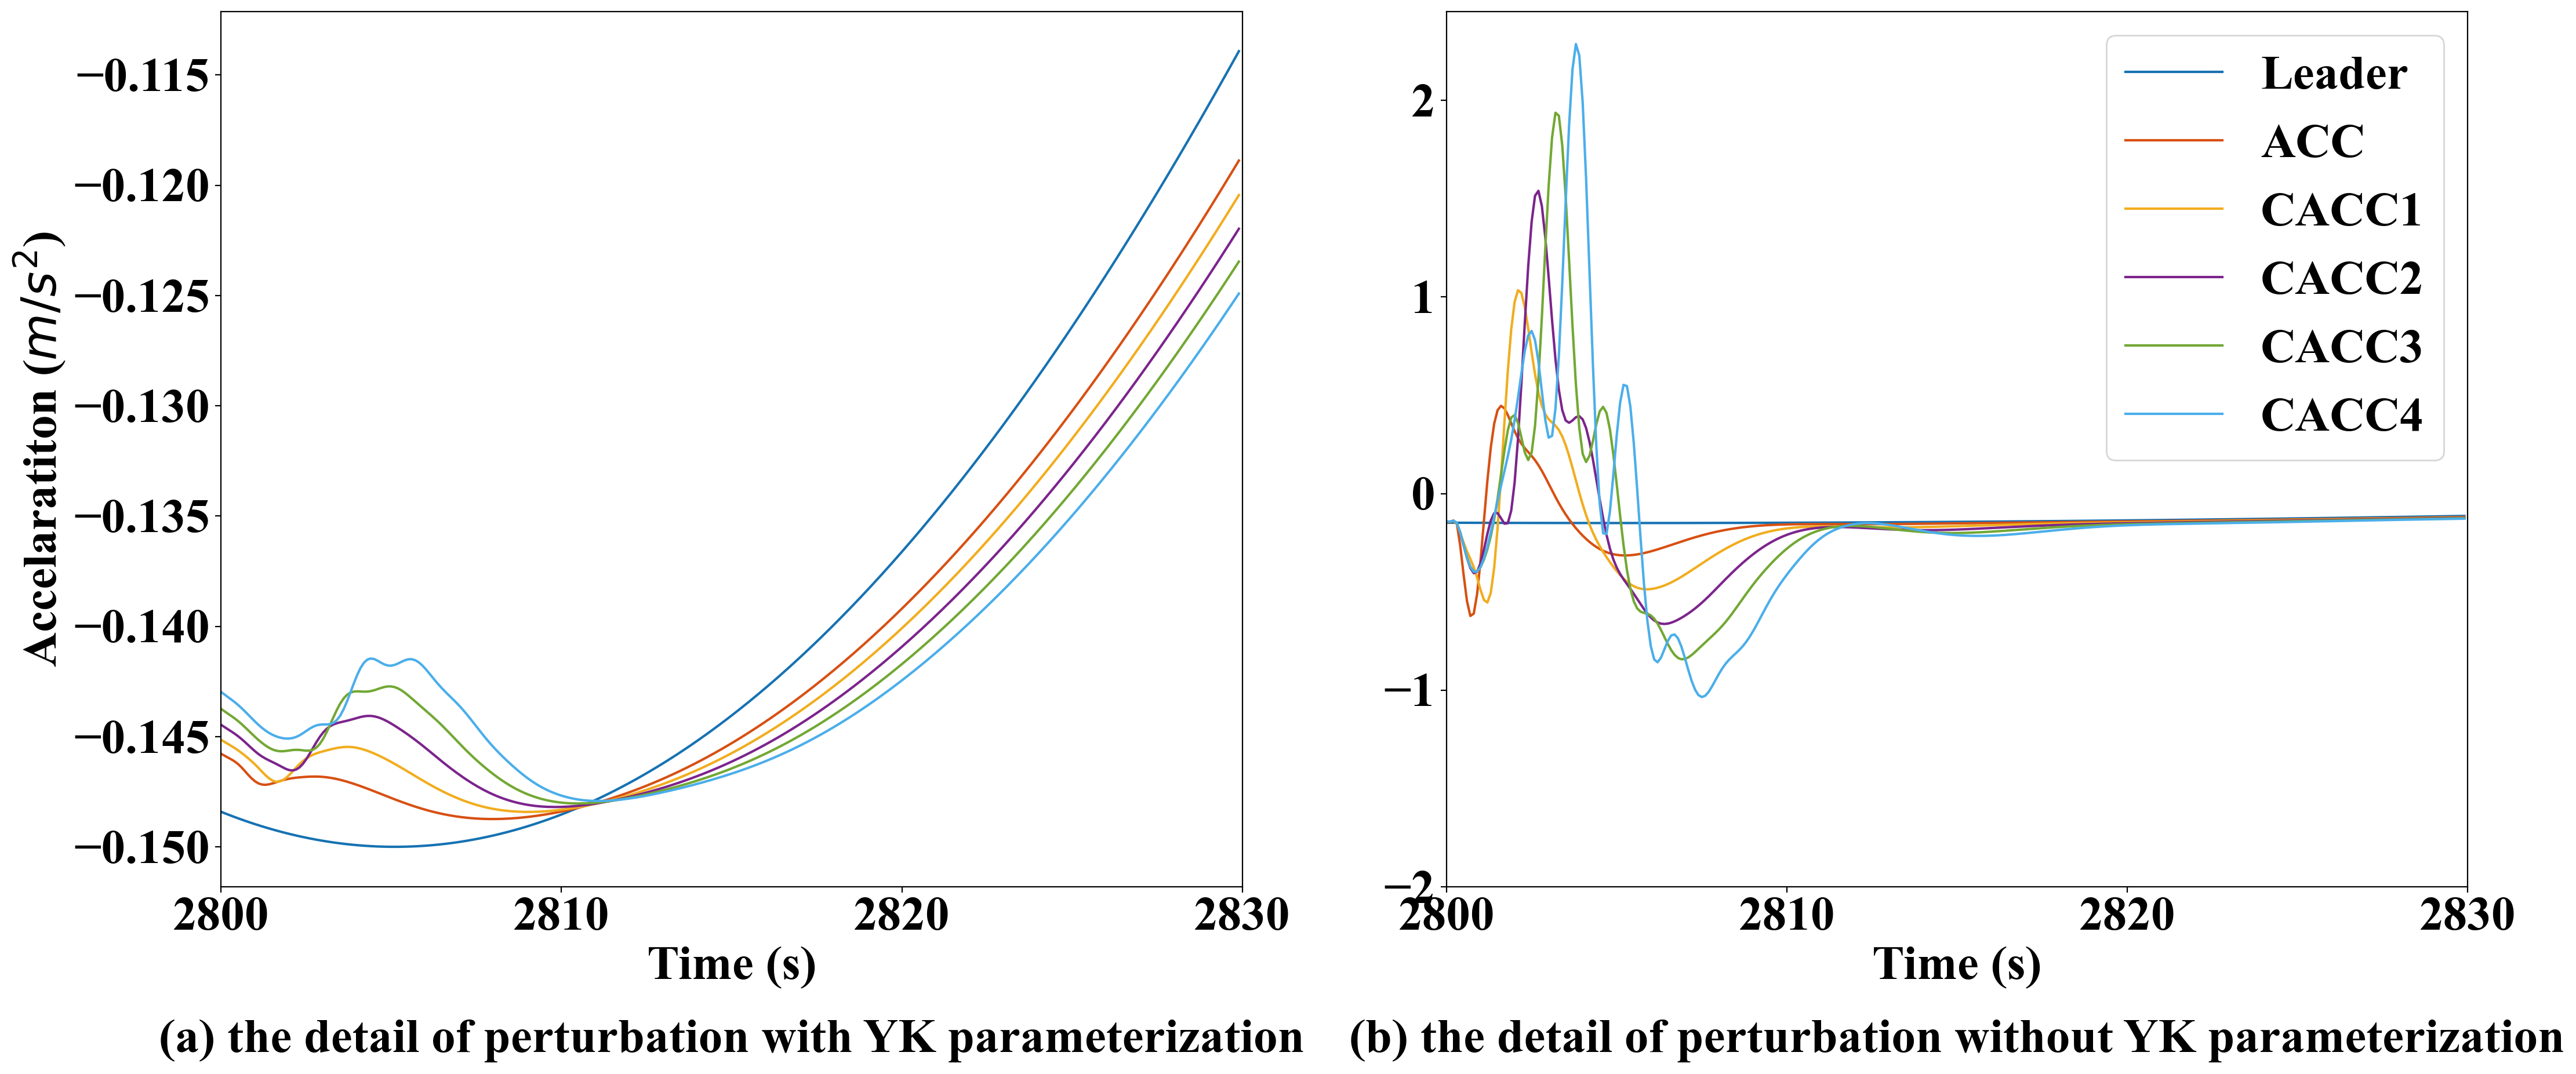
\includegraphics[width=14cm]{figs/extendfig6.png}
% 	\caption{~Detailed perturbation simulation results of experiment five and six: CACPC with or without YK parameterization.}
% 	\label{extend6}
% \end{figure}

\textit{Simulation results}. Figure.~\ref{new5}, \ref{new6} show the results of experiments five and six from global and local perspective respectively. The format of figure.~\ref{new5}, \ref{new6} is same as figure.~\ref{new1}, \ref{new2}. For the sake of simplicity, the detailed introduction is omitted. In Figure.~\ref{new5}, the top graph plots the vehicles' accelerations, the median graph plots the vehicles' velocities during the simulation, and the bottom graph plots the time gap during the simulation in each figure.

From the figure.~\ref{new5}, the simulation results under the traffic oscillation scenario are similiar to the results with constant velocity. The corresponding detailed simulation results are shown in figure.~\ref{new6}. The spontaneous perturbations caused by the controller switching are not significant which have the magnitude of 0.015 $m/s^2$ with the YK parameterization while the perturbation have the magnitude of 2.15$m/s^2$ for the case without YK parameterization under the traffice oscillation scenario. And a noticeable rise appears in the speed graph which means a significant negative impact on traffic safety. A conclusion can be drawn that the YK parameterization can ensure the smooth switching of the controllers whether it is traffic oscillation or equilibrium state.

\subsubsection{Simulation experiments maintain a constant speed during the multiple CACCs forming process}
\label{Section 5.2.3}

\textit{Simulation scenario:} The simulation scenario of experiment seven is set as: at first, a leader vehicle drives on an infinitely long road under a given speed and acceleration configuration which is similiar to the experiment one in Section. ~\ref{Section 5.2.1}. There is only three perturbations at the simulation time of 300s, 1000s and 1700s. And the forming process of the CACC platoon is that two CACCs join in the ACC platoon at the same time, and the forming process repeat twice at the simulation time of 700s and 1400s. Notice that only the case with YK parameterization is applied is simulated here because simulation results of the case without YK parameterization is similiar to the experiment two in Section. ~\ref{Section 5.2.1}.

\begin{figure}[htb]
  \centering
  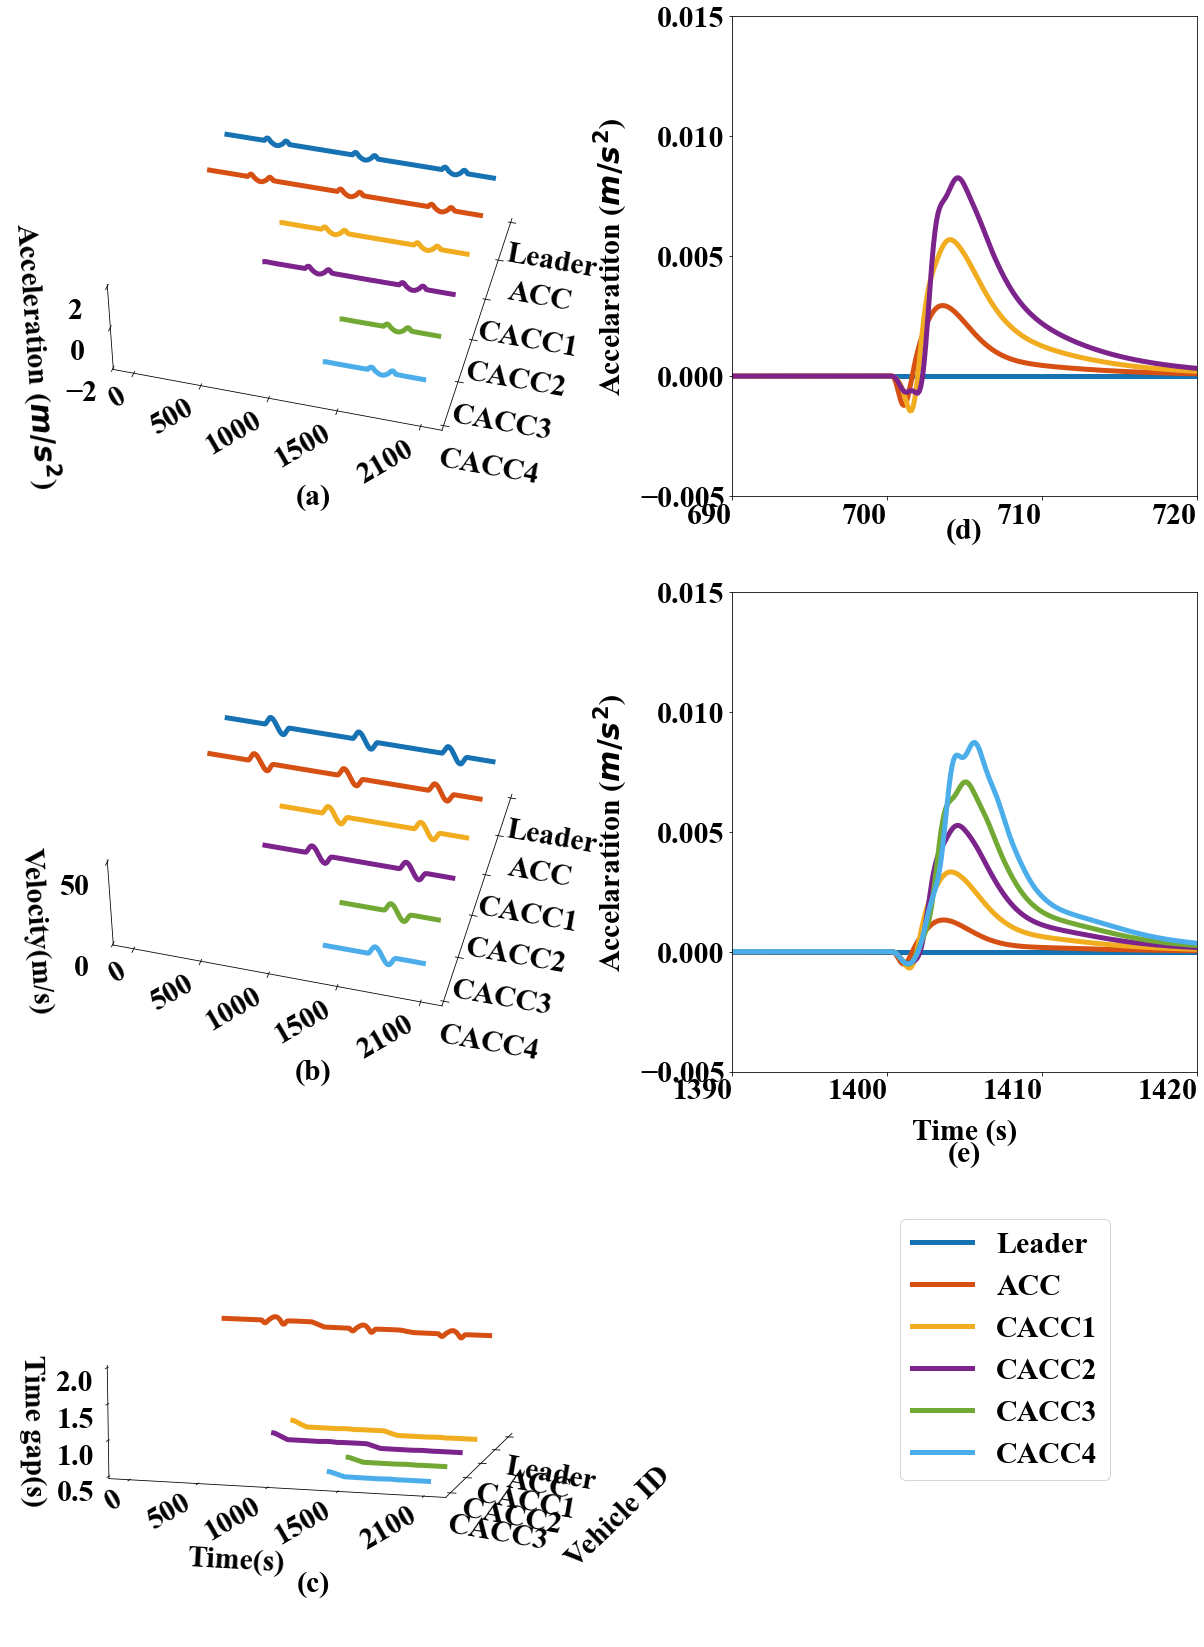
\includegraphics[width=10cm]{figs/extendfig7.png}
  \caption{~Simulation results of experiment seven: CACPC with YK parameterization under multiple CACCs forming at the same time. (a) Acceleration of simulation results; (b) Velocity of simulation results; (c) Time gap of simulation results; (d) Detailed acceleration of simulation results in 690-720s; (e) Detailed acceleration of simulation results in 1390-1420s}
  \label{extend7}
\end{figure}

\textit{Simulation results}. Figure.~\ref{extend7} shows the results of experiments seven. In the left subplot, the top graph plots the vehicles' accelerations, the median graph plots the vehicles' velocities during the simulation, and the bottom graph plots the time gap during the simulation. And the right subplot show the detailed accelaration in 690-720s and 1390-1420s to explore the spontaneous perturbation during controllers switching.

Form figure.~\ref{extend7}, the first conclusion can be drawn that YK parameterization can keep string stability even during the multiple CACCs forming process. The second conclusion can be found from figure.~\ref{extend7} (d) and (e) that the spontaneous perturbation caused by controllers switching is amplified with multiple CACCs forming. However, the magnitude of the first switching perturbation is still only 0.015 $m/s^2$ which is significantly lower than the case without YK parameterization.






% \subsection{Simulation experiments of the capacity}
% \label{Section 5.3}

% There is no doubt that the most effective and most intuitive indicator for evaluating traffic flow is capacity. Therefore, the trends of traffic capacity with and without CACPC are compared through simulation experiments. In addition, CACC MPR is also considered in simulation experiments because CAV-MV heterogeneous traffic flow will continue to exist for a long time. The simulation results are shown in Figure.~\ref{fig13}.

% \begin{figure}
% 	\centering
% 		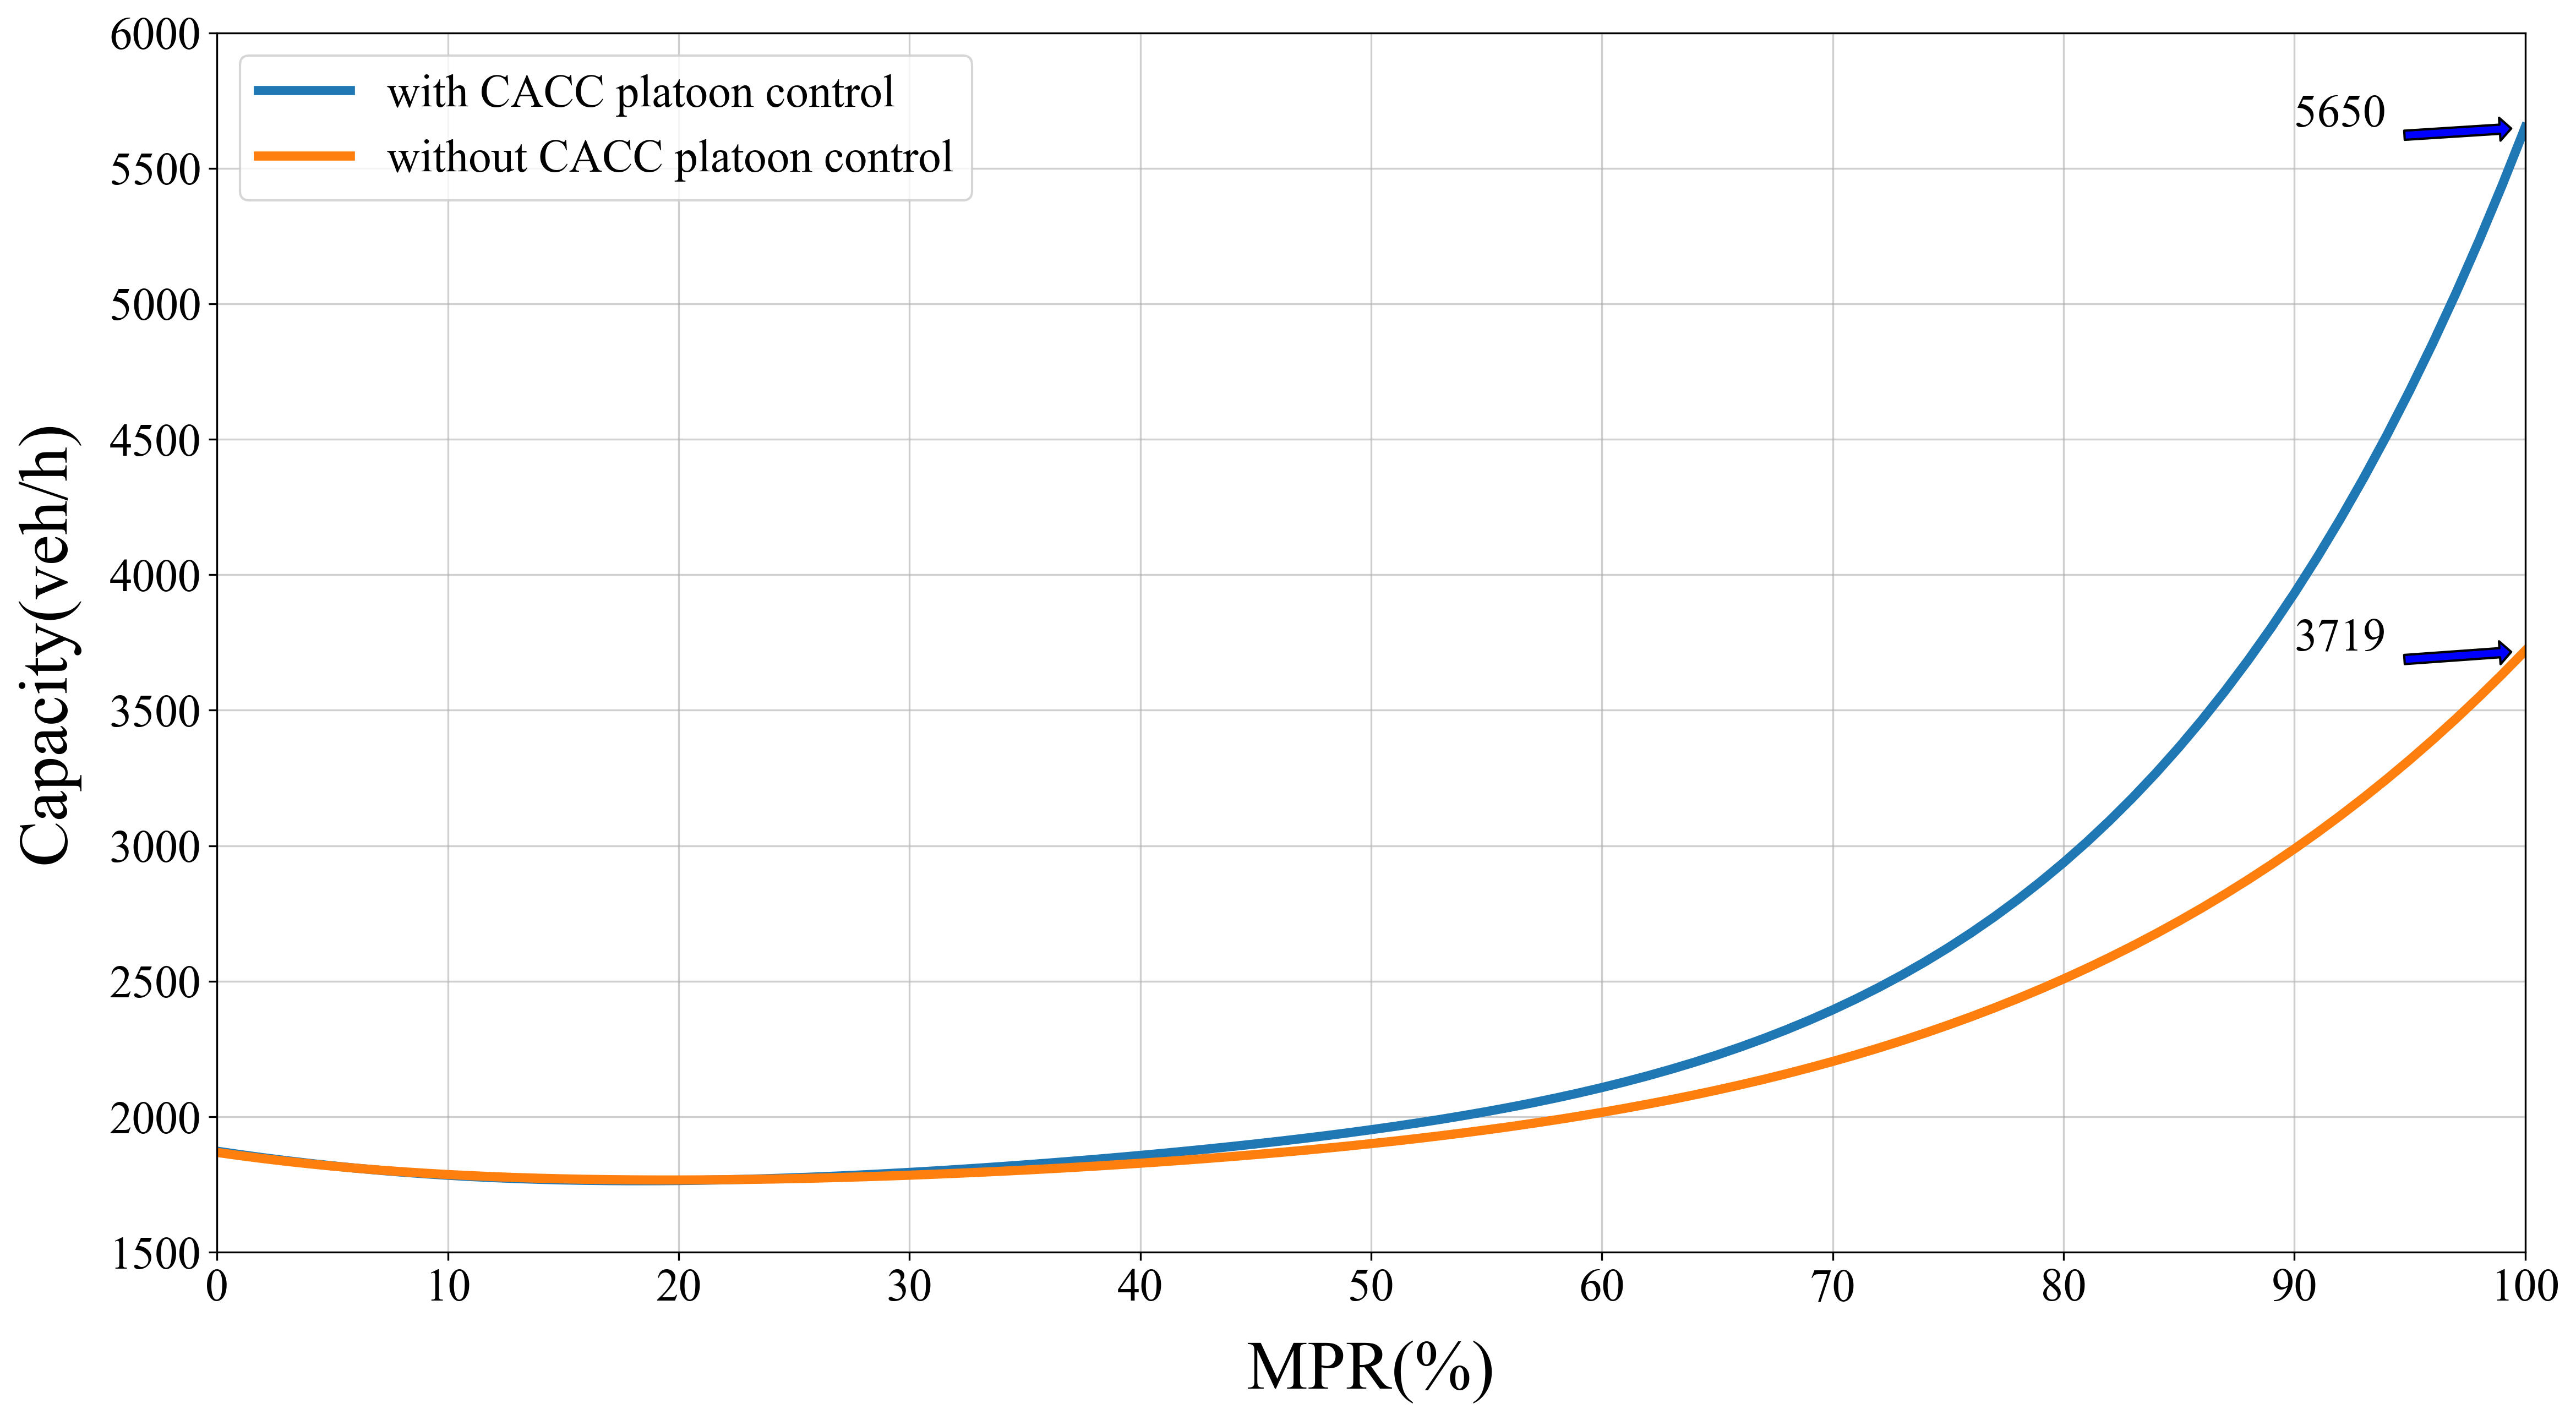
\includegraphics[width=14cm]{figs/fig13.png}
% 	\caption{~Simulation results of the capacity with or without CACPC under different MPR.}
% 	\label{fig13}
% \end{figure}

% A conclusion can be drawn from Figure.~\ref{fig13} that the capacity first increases and then decreases with CAV MPR increasing. It can be found that it will no longer keep the same capacity as the pure MV scenario when the MPR reaches 42\%. When we pay attention to the benefit of CAV involvement on the capacity, we find that as the MPR increases, the capacity gain becomes more obvious, and when the MPR reaches 100\%, the capacity can reach 5650 veh/h, which is 3.02 times that of the pure MV scenario. Moreover, the use of CACPC can improve capacity, and the capacity gain of CACPC will gradually become more significant as the MPR increases since platoon is more likely to form in the case of high MPR. When the MPR is 100\%, the capacity with CACPC can reach 1.52 times that of the situation without it. From the above analyses, we can conclude that the adoption of CACPC can significantly benefit the traffic capacity, especially under high MPR.

\section{Conclusion}
\label{Section 6}

This paper proposes a control mode called CACPC to further improve the capacity by regarding the whole CACC platoon as the control object instead of a single vehicle. In this control mode, string stability of the CACC platoon is analyzed to get the margin desired time gap under different platoon sizes. Then YK parameterization is applied to ensure string stability of the CACC platoon when the CACC is switching from single vehicle control mode to platoon control mode, and the corresponding tuning function is proposed so that the specific platoon size does not limit the application range of this control mode. Moreover, the effectiveness of CACPC has been explored from two aspects: the impact of YK parameterization on dynamic performance of CACPC. The following conclusions can be drawn through this paper:
\begin{enumerate}
  \item A new control mode is proposed to control the whole CACC platoon instead of a single vehicle.
  \item CACPC is composed of two CACC controllers. YK parameterization ensures the stable interpolation between the two to guarantee smooth switching and string stability.
  \item Combination of tuning function $\gamma$ under different platoon sizes is derived by ensuring that the application range of CACPC is not limited by platoon size.
  \item Adopting YK parameterization can significantly suppress the spontaneous perturbation from 2$m/s^2$ to 0.015$m/s^2$ caused by the controller switch.
  \item YK parameterization can ensure smooth controller switching under the equilibrium state, traffic oscillation, and multiple CACCs forming.
\end{enumerate}



\appendix
\section*{Appendix A. System identification of lower level controller based on field experiments}
\label{AppendixA}

\textit{Experiment preparation}: The experiment was conducted at Closed test site of National Smart CAV \& C-ITS (Beijing + Hebei) Demonstration Zone Shunyi Base on March 29, 2021. Two cycabs were used for experiment which were autonomous driving vehicles developed by iDriverplus technology company. The scheme of LiDAR+ millimeter wave + Ultrasonic radar + GPS inertial navigation was adopted as the navigation system, and the distance measurement accuracy is 0.05m. The decision frequency is 20 Hz which equals to a 50ms decision interval. The figure.~\ref{experiment} show the scene of the field experiment.

\begin{figure}
  \centering
  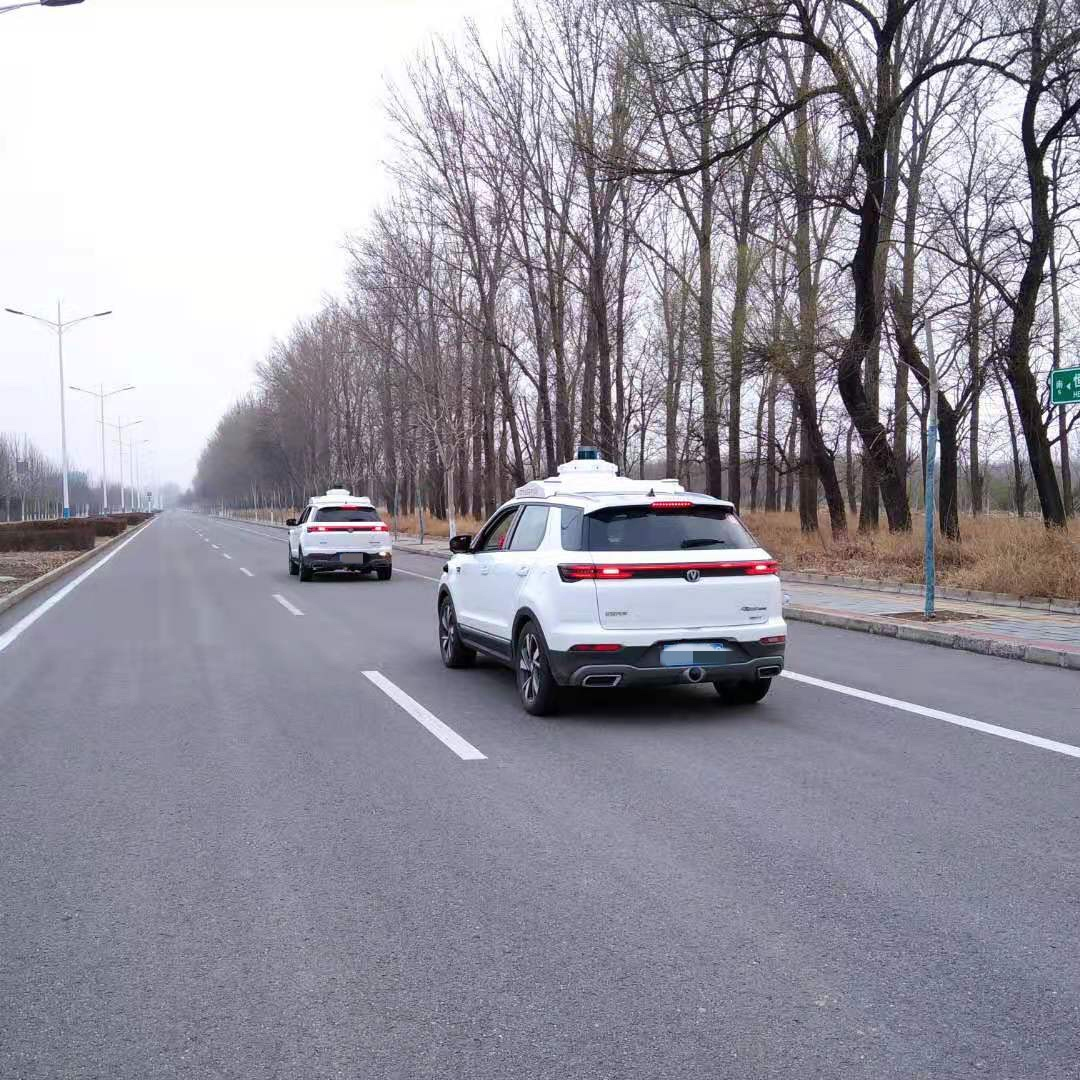
\includegraphics[width=14cm]{figs/experiment.jpg}
  \caption{~Field experiment scene.}
  \label{experiment}
\end{figure}

\textit{Experiment scheme}: The experiments was divided into 5 groups. Each group had several rounds, which amounted to a total of 21 rounds of experiments. In each round, the front car drove in accordance with the speed configuration while the back car used the longitudinal control of ACC system to follow the front car and recorded the actual acceleration of the back car. Different groups used different control parameters of ACC system to ensure that a general conclusion can be drawn.

The control parameters of ACC system in different experiment groups are as follows:
\begin{table}
  \caption{~Parameters chosen for different experiment groups.}
  \begin{tabular}{ccccc}
    \hline Index of experiments group & $k_{p}$               & $k_{d}$              & $h_{i}$           & round \\
    \hline $1^{\text {st }}$          & $0.7 \mathrm{s}^{-2}$ & $0  \mathrm{s}^{-1}$ & $2 \mathrm{~s}$   & 2     \\
    \hline $2^{\text {nd }}$          & $0.5 \mathrm{s}^{-2}$ & $0  \mathrm{s}^{-1}$ & $1.8 \mathrm{~s}$ & 5     \\
    \hline $3^{\text {rd }}$          & $0.6 \mathrm{s}^{-2}$ & $0  \mathrm{s}^{-1}$ & $2 \mathrm{~s}$   & 7     \\
    \hline $4^{\text {th }}$          & $0.7 \mathrm{s}^{-2}$ & $0  \mathrm{s}^{-1}$ & $2 \mathrm{~s}$   & 4     \\
    \hline $5^{\text {th }}$          & $0.4 \mathrm{s}^{-2}$ & $0  \mathrm{s}^{-1}$ & $2 \mathrm{~s}$   & 3     \\
    \hline
  \end{tabular}
  \label{table 2}
\end{table}

The experiment data of command acceleration and actual acceleration in first round are shown in figure.~\ref{fig14}, where $a_{cmd}$ means the command acceleration and $a_{actual}$ means the actual acceleration.

\begin{figure}
  \centering
  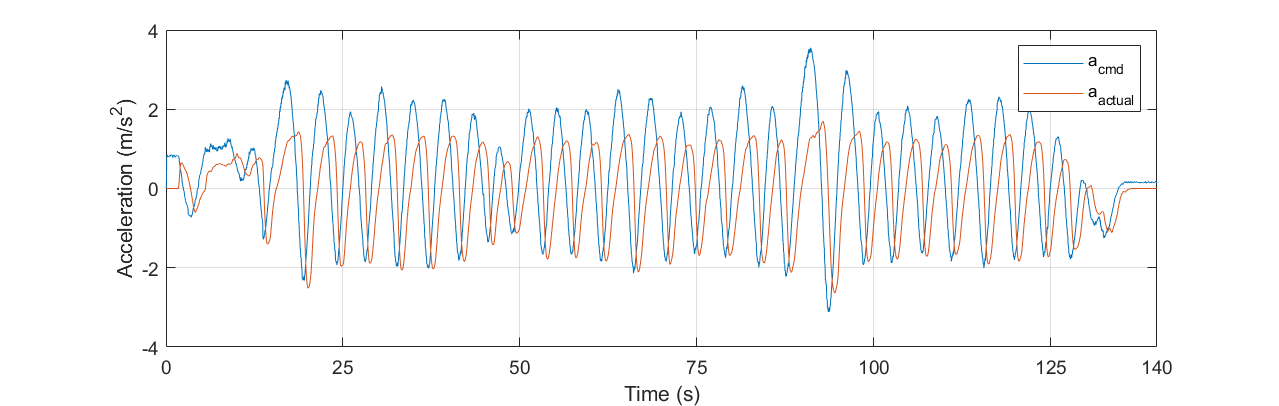
\includegraphics[width=14cm]{figs/fig14.png}
  \caption{~Experiment data of the command acceleration and the actual acceleration in first round, where $a_{cmd}$ means the command acceleration and $a_{actual}$ means the actual acceleration.}
  \label{fig14}
\end{figure}

In order to calibrate the transfer function of the lower controller $G_s (s)$, the command acceleration and actual acceleration of the back car in each round are regarded as input and output respectively. Notice that since the output of the lower controller $G_s (s)$ in figure.~\ref{fig2} is position instead of acceleration, additional second-order integration is applied. Using the System Identification toolbox in MATLAB and setting desire system type, the transfer function is fitted as follows:
\begin{equation}
  G_{i}(s)=\frac{k_{G}}{s^{2}\left(\tau_{i} s+1\right)} e^{-\phi_{i} s}=\frac{0.9403}{s^{2}(0.7862 s+1)} e^{-0.2 s},
\end{equation}
which keeps fit error to minimun: FPE=0.08699 and MSE=0.0868.

\section*{Appendix B. Proof of the Equation (\ref{Eq17}-\ref{Eq18})}
\label{AppendixB}

The Equation (\ref{Eq17}-\ref{Eq18}) must satisfy the following identities:

\begin{enumerate}[(a)]
  \item $G=N M^{-1}=\tilde{M}^{-1} \tilde{N}$,
  \item $K_{i}=U_{i} V_{i}^{-1}=\tilde{V}_{i}^{-1} \tilde{U}_{i}$,
  \item    $ \left[\begin{array}{cc}
              \tilde{V}_{i} & -\tilde{U}_{i} \\
              -\tilde{N}    & \tilde{M}
            \end{array}\right]\left[\begin{array}{cc}
              M & U_{i} \\
              N & V_{i}
            \end{array}\right]=\left[\begin{array}{cc}
              M & U_{i} \\
              N & V_{i}
            \end{array}\right]\left[\begin{array}{cc}
              \tilde{V}_{i} & -\tilde{U}_{i} \\
              -\tilde{N}    & \tilde{M}
            \end{array}\right]=\left[\begin{array}{cc}
              I & 0 \\
              0 & I
            \end{array}\right].$
\end{enumerate}


\textbf{Proof.} Proof of (a) $G=\tilde{M}^{-1} \tilde{N}$:

\begin{equation}
  \begin{aligned}
    \tilde{M}^{-1} \tilde{N}=
     & \left[\begin{array}{cc|c}
        A+B D_{i}^{c} C & B    C_{i}^{c} & B    D_{i}^{c} \\
        B_{i}^{c}   C   & A_{i}^{c}      & B_{i}^{c}      \\
        \hline   C      & -F_{i}^{c}     & I              \\
      \end{array}\right]^{-1} \left[\begin{array}{cc|c}
        A+B    D_{i}^{c} C & B    C_{i}^{c} & B \\
        B_{i}^{c}   C      & A_{i}^{c}      & 0 \\
        \hline    C        & -F_{i}^{c}     & 0 \\
      \end{array}\right] \\
     & =\left[\begin{array}{cc|c}
        A          & B    (C_{i}^{c}+D_{i}^{c}F_{i}^{c}) & -B    D_{i}^{c} \\
        0          & A_{i}^{c}+B_{i}^{c}  F_{i}^{c}      & -B_{i}^{c}      \\
        \hline   C & -F_{i}^{c}                          & I               \\
      \end{array}\right]  \left[\begin{array}{cc|c}
        A+B    D_{i}^{c} C & B    C_{i}^{c} & B \\
        B_{i}^{c}   C      & A_{i}^{c}      & 0 \\
        \hline    C        & -F_{i}^{c}     & 0 \\
      \end{array}\right]    \\
    % 开始写两矩阵相乘
     & =\left[\begin{array}{cccc|c}
        A          & B    (C_{i}^{c}+D_{i}^{c}F_{i}^{c}) & -B    D_{i}^{c}C   & B    D_{i}^{c}F_{i}^{c} & 0 \\
        0          & A_{i}^{c}+B_{i}^{c}   F_{i}^{c}     & -B_{i}^{c}  C      & B_{i}^{c}  F_{i}^{c}    & 0 \\
        0          & 0                                   & A+B    D_{i}^{c} C & B    C_{i}^{c}          & B \\
        0          & 0                                   & B_{i}^{c}   C      & A_{i}^{c}               & 0 \\
        \hline   C & -F_{i}^{c}                          & C                  & -F_{i}^{c}              & 0 \\
      \end{array}\right]                                             \\
     & =\left[\begin{array}{cccc|c}
        A          & B    (C_{i}^{c}+D_{i}^{c}F_{i}^{c}) & 0                  & 0           & B \\
        0          & A_{i}^{c}+B_{i}^{c} F_{i}^{c}       & 0                  & 0           & 0 \\
        0          & 0                                   & A+B    D_{i}^{c} C & B C_{i}^{c} & B \\
        0          & 0                                   & B_{i}^{c}   C      & A_{i}^{c}   & 0 \\
        \hline   C & -F_{i}^{c}                          & 0                  & 0           & 0 \\
      \end{array}\right]                                            \\
    % 补充矩阵讲解推导公式
     & =\left[\begin{array}{c|c}
        A        & B \\
        \hline C & 0 \\
      \end{array}\right] ,
  \end{aligned}
  % \label{Eq18}
\end{equation}
where $\mathbf{T}=\left[\begin{array}{cccc}\mathbf{I} & 0 & -\mathbf{I} & 0 \\ 0 & \mathbf{I} & 0 & -\mathbf{I} \\ 0 & 0 & \mathbf{I} & 0 \\ 0 & 0 & 0 & \mathbf{I}\end{array}\right], \quad \mathbf{T}^{-1}=\left[\begin{array}{cccc}\mathbf{I} & 0 & \mathbf{I} & 0 \\ 0 & \mathbf{I} & 0 & \mathbf{I} \\ 0 & 0 & \mathbf{I} & 0 \\ 0 & 0 & 0 & \mathbf{I}\end{array}\right]$  is adopted in the similarity transformation.
The proofs that $G=N M^{-1}$ and (ii) are analogous.

\textbf{Proof.} Proof of (c) $\left[\begin{array}{cc}
      M & U_{i} \\
      N & V_{i}
    \end{array}\right]\left[\begin{array}{cc}
      \tilde{V}_{i} & -\tilde{U}_{i} \\
      -\tilde{N}    & \tilde{M}
    \end{array}\right]=\left[\begin{array}{cc}
      I & 0 \\
      0 & I
    \end{array}\right].$

\begin{equation}
  \begin{aligned}
     & \left[\begin{array}{cc}
        M & U_{i} \\
        N & V_{i}
      \end{array}\right]^{-1}  \\
     & =\left[\begin{array}{cc|cc}
        A+B F     & 0                             & -B & 0         \\
        0         & A_{i}^{c}+B_{i}^{c} F_{i}^{c} & 0  & B_{i}^{c} \\
        \hline -F & C_{i}^{c}+D_{i}^{c} F_{i}^{c} & I  & D_{i}^{c} \\
        -C        & F_{i}^{c}                     & 0  & I
      \end{array}\right]^{-1} \\
     & =\left[\begin{array}{cc|cc}
        A+B  D_{i}^{c} C          & B  C_{i}^{c} & -B & B  D_{i}^{c} \\
        B_{i}^{c} C               & A_{i}^{c}    & 0  & B_{i}^{c}    \\
        \hline F_{i}- D_{i}^{c} C & -C_{i}^{c}   & I  & -D_{i}^{c}   \\
        C                         & -F_{i}^{c}   & 0  & I            \\
      \end{array}\right]      \\
     & =\left[\begin{array}{cc}
        \tilde{V}_{i} & -\tilde{U}_{i} \\
        -\tilde{N}    & \tilde{M}
      \end{array}\right].
  \end{aligned}
\end{equation}

\textbf{Q.E.D.}


\printcredits

\section*{Acknowledgment}

This research was sponsored by the National Key Research and Development Program of China (No. 2019YFB1600200), National Science Foundation of China (No. 51878161, No. 71931002 and No.52072067).

%% Loading bibliography style file
% \bibliographystyle{model1-num-names}
\bibliographystyle{cas-model2-names}

% Loading bibliography database
\bibliography{cas-refs}


%\vskip3pt

\end{document}

